\documentclass{report}
\usepackage[utf8]{inputenc}
\usepackage[english]{babel}
\usepackage{graphicx}
\usepackage{amsmath}
\usepackage{parskip}
\parskip=2\baselineskip \advance\parskip by 0pt plus 1pt

\newcommand{\analysis}{the \href{http://analysis.sns.gov}{Analysis} machine}

\newcommand{\cmd}[1]{\texttt{#1}}
\newcommand{\addiecmd}{\cmd{fastgr}}

\newcommand{\fileio}[1]{\texttt{#1}} 
\newcommand{\iptsPrint}{\fileio{/SNS/NOM/IPTS-<your experiment ID>}}

\newcommand{\guicmd}[1]{\textbf{\textit{#1}}}
 
\newcommand{\snspowderreduction}{\href{http://docs.mantidproject.org/nightly/algorithms/SNSPowderReduction-v1.html}{SNSPowderReduction}}
 
\usepackage[pdfpagelabels]{hyperref}
\hypersetup{
    colorlinks=true,
    linkcolor=blue,
    filecolor=magenta,      
    urlcolor=red,
}
 
\urlstyle{same}
 
\begin{document}

{\let\cleardoublep
\clearpage 
\begin{titlepage}
	\centering
	
\includegraphics[width=0.75\textwidth]{graphics/joke_image.jpg}\par\vspace{1cm}
	\vspace{2cm}
	{\huge\bfseries ADDIE User Manual\par}
	{\LARGE\bfseries\itshape ADvanced DIffraction Environment\par}
	\vspace{1cm}
	{\Large\bfseries\ Data reduction software for NOMAD\par}
	\vfill
	{\large\bfseries \today{} version \par}
\end{titlepage}
 

 \tableofcontents
 \addtocontents{toc}{~\hfill\textbf{Page}\par}

}

\chapter{Introduction}
\section{What is ADDIE} 
The ADvanced DIffraction Environment (ADDIE) is User software for 
reducing and analyzing data on the  
\href{http://https://neutrons.ornl.gov/nomad}{Nanoscale Ordered MAterials Diffractometer}  (NOMAD)  instrument at the \href{https://neutrons.ornl.gov/sns}{Spallation Neuron Source} (SNS). 
Now, with a full plate of acronyms, let's begin.


ADDIE provides a graphical user interface (GUI) to interact with the 
underlying data reduction software. ADDIE aims to guide the workflow to 
go from launching the reduction of raw neutron data to provided processed 
individual runs, post-processing of these individual runs  by applying 
optional corrections and summations, finally to visualization and 
output of the diffraction and pair distribution function data. 

ADDIE in pre-installed on \analysis at the SNS 
(\url{http://analysis.sns.gov}). Instructions are provided for Neutron Sciences users 
to setup the Remote Desktop capablities to view, analyze and download your data 
from anywhere you go. Options are provided Windows, Mac, and Linux. 
Also, contact support information is provided in the case of 
any issues or needed troubleshooting.

ADDIE is also avaible open-source. 
Please contact your Local Contact from NOMAD if you would like to 
know more about the repository (or to contribute!)
\section{Using ADDIE}

ADDIE development has been funded by the 
\href{https://www.energy.gov/}{US Department of Energy} (DOE). 

If you use ADDIE results in your published work, please cite the following papers:

(INSERT - ADDIE paper)
(INSERT - other reduction dependencies - Mantid, GUDRUN, etc.)

For any of the following features for your published work, please cite the associated papers:

(INSERT - specific feature papers)

From the following, you can download a \href{http://https://neutrons.ornl.gov/nomad}{BibTex file with all citations}.


 
\chapter{Getting Started}
\section{Background}

What does ADDIE actually do during data reduction? For each run, we must have the following measurements for data reduction:

\begin{equation} \label{eq_intensities}
\begin{split}
I_{sample}  & = \text{sample intensity} \\
I_{C}  & = \text{sample container intensity} \\
I_{Cb} & = \text{container background intensity} \\
I_{V}  & = \text{vanadium intensity} \\
I_{Vb} & = \text{vanadium background intensity} 
\end{split}
\end{equation}

Why all these measurements for a single run? We want to measure only the coherent sample scattering ($I_{sample}^{coh}$). Unfortunately, we cannot suspend the sample in space inside the instrument. We must have a sample container. Thus, we measure the empty sample container intensity ($I_{C}$) in the instrument to subtract this from the sample scattering intensity ($I_{sample}$). Yet, we can have many different types of "containers" (i.e. sample environments such as a furnace or cryostat, vanadium cans, quartz tubes, tubes in cans, etc.) Therefore, we must correct "from the outside in" where we subtract a completely empty instrument from the outermost containment scattering intensity, then subtract this from the next layer of containment and continue till we reach the sample subtracted ($I_{sample}$) from this collective background ($I_{C} + I_{Cb}$).  Also, we do not know the exact beam profile to put the sample scattering intensity on an absolute scale. For this, we use vanadium to normalize the sample scattering intensity to extract the coherent scattering ($I_{sample}^{coh}$) from the incoherent scattering ($I_{sample}^{inc}$) on an absolute scale. 

Why vanadium for normalization? We use vanadium for a few different reasons. 1) Vanadium has a small coherent scattering length but is a great incoherent scattering material. Thus, it does not contain large Bragg reflections in its profile that would have to be removed but provides a well-defined total beam profile. 2) Vanadium is a solid metal with well known density and stable without a container. 3) The large mass of vanadium atoms reduces the need to correct for inelastic scattering effects.

What else before we get our coherent sample intensity? Last, we must take into account the loss of intensity of the neutron beam as it passes through every material present in the experiment. To some degree, the sample, container, and vanadium will all attenuate the neutron beam. Ignoring the sample attenuation, we have: 

\begin{equation} \label{eq_reduction}
\begin{split}
I_{sample}^{coh} & = \frac{I_{sample}-\alpha_c (I_{C}-I_{Cb})}{\alpha_v(I_{V}-I_{Vb})}  
\end{split}
\end{equation}

From the coherent scattering, we have the total scattering structure function given as:

\begin{equation} \label{eq_reduction}
\begin{split}
S(Q) - 1 & = \frac {\frac{I_{sample}^{coh}}{N} - \langle b^2 \rangle }{{{\langle b \rangle}^2 }} \\
         & = \frac {\frac{d \sigma}{d \Omega}  - \langle b^2 \rangle }{{{\langle b \rangle}^2 }} \\
         & = 
\end{split}
\end{equation}

where ${\langle b \rangle}^2$ and $\langle b^2 \rangle$ are the squared average and average squared scattering power of the sample where:

\begin{equation} \label{eq_reduction}
\begin{split}
\langle b \rangle = \frac {\sum_{i}^{N} b_{i}}{N}
\end{split}
\end{equation}


where $b_i$ is the scattering power of atom $i$ and $N$ is the total number of atoms in the sample.

The pair distribution function (PDF) is obtained from the Fourier transform of $S(Q)-1$:

\begin{equation} \label{eq_reduction}
\begin{split}
G(r) = \frac{2}{\pi} \int_{\inf}^{0} Q [S(Q)-1] \text{sin}(Qr) dQ
\end{split}
\end{equation}

\section{Specifics of NOMAD data reduction}

To obtain $S(Q)$ we using the following:

\begin{equation} \label{eq_reduction}
\begin{split}
S(Q) - 1 = \frac{\frac{I_{sample}^{coh}}{N} - I_{poly}}{I_poly}
\end{split}
\end{equation}

where 
\begin{equation} \label{eq_reduction}
I_{poly} = \begin{cases} 
      		\frac{\rho \sigma \}{} & x\leq 0 \\
      		\frac{100-x}{100} & 0\leq x\leq 100 \\
      		0 & 100\leq x 
		 \end{cases}
\end{equation}
\chapter{Workflow for Data Reduction}
To launch ADDIE, you must:
\begin{enumerate}
\item Login to \analysis
\item Open a terminal
\item Navigate to your IPTS. It will be located on Analysis under \iptsPrint
\item Launch ADDIE using the command: \addiecmd
\item Wait for the GUI to appear

\end{enumerate}
\section{Launch reduction of individual runs}
\subsection{Load input}

\section{Post-Processing of runs}
\subsection{Load Runs into Table}

After we have ran the autoreduction, we can begin Post-Processing of the data. On the Post-Processing Tab, we have the following:

\noindent\makebox[\textwidth]{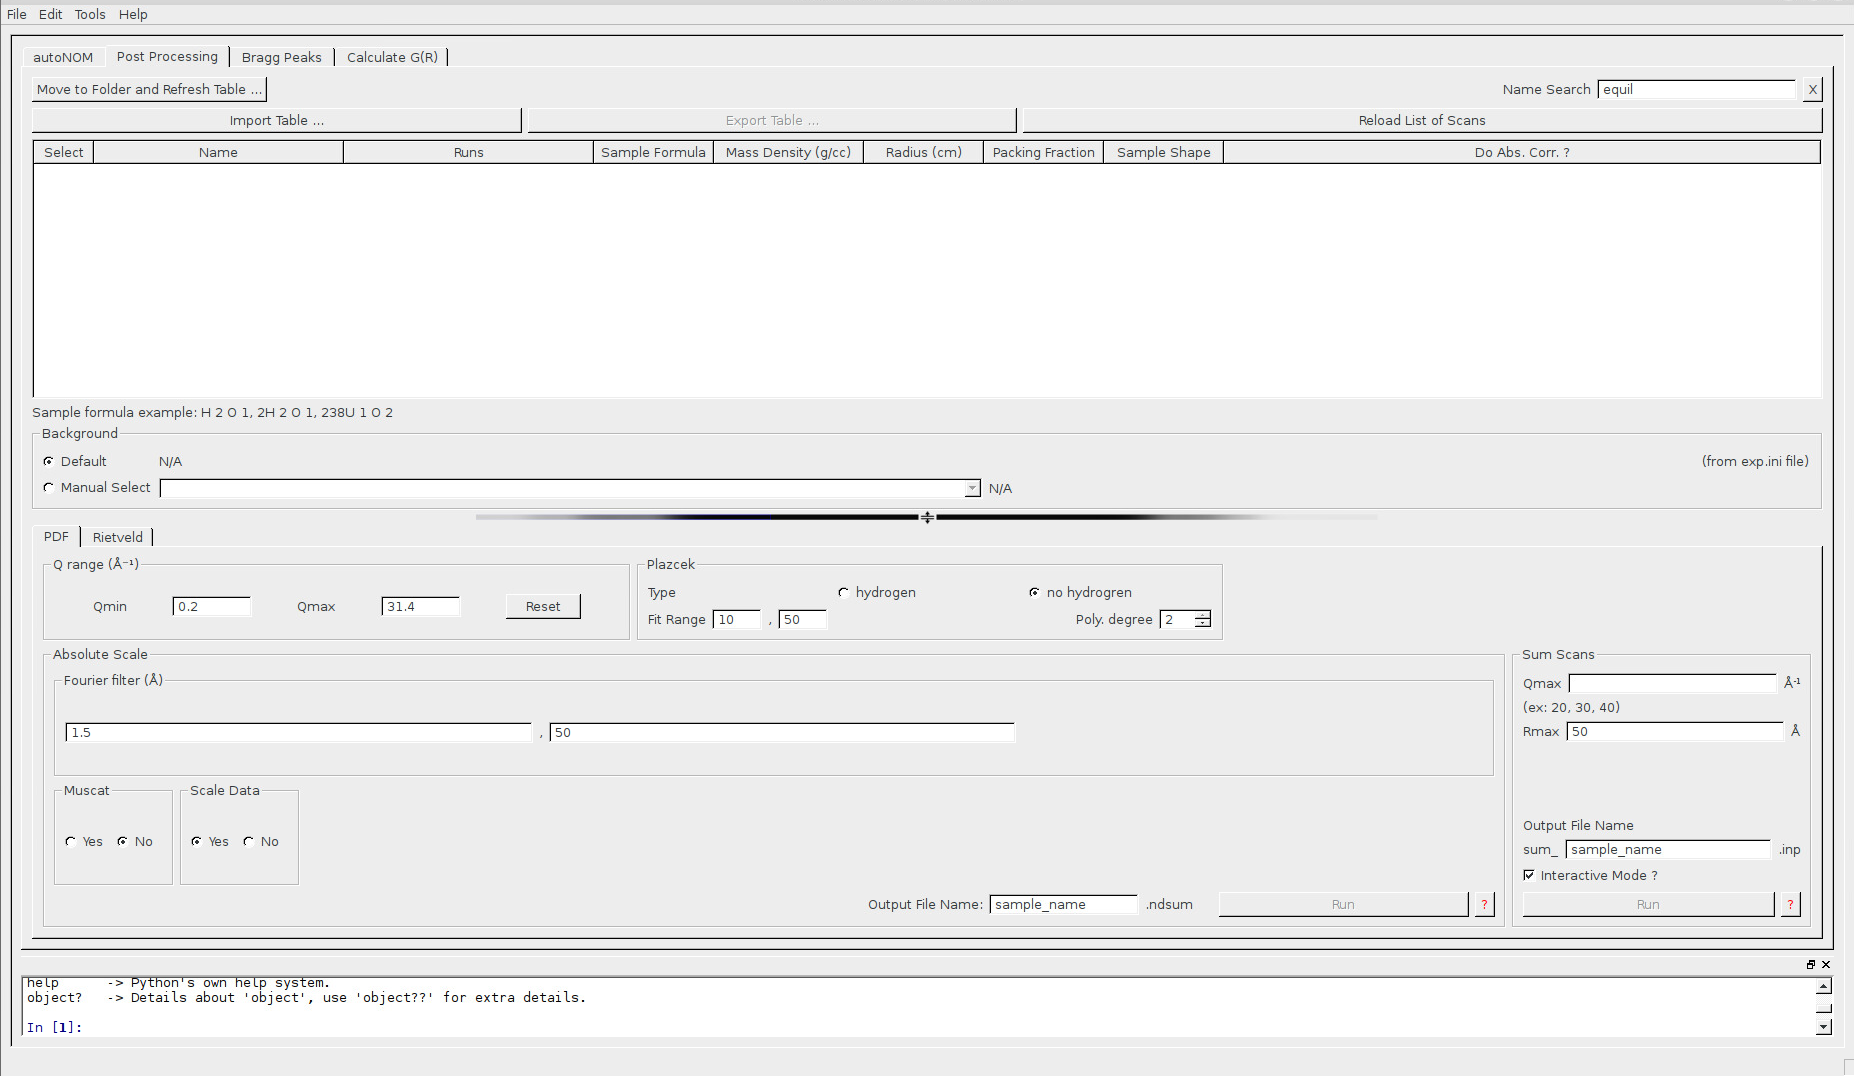
\includegraphics[width=0.9\paperwidth]{graphics/tab2/tab2.png}}

From here we can import data from our runs into the table:

\noindent\makebox[\textwidth]{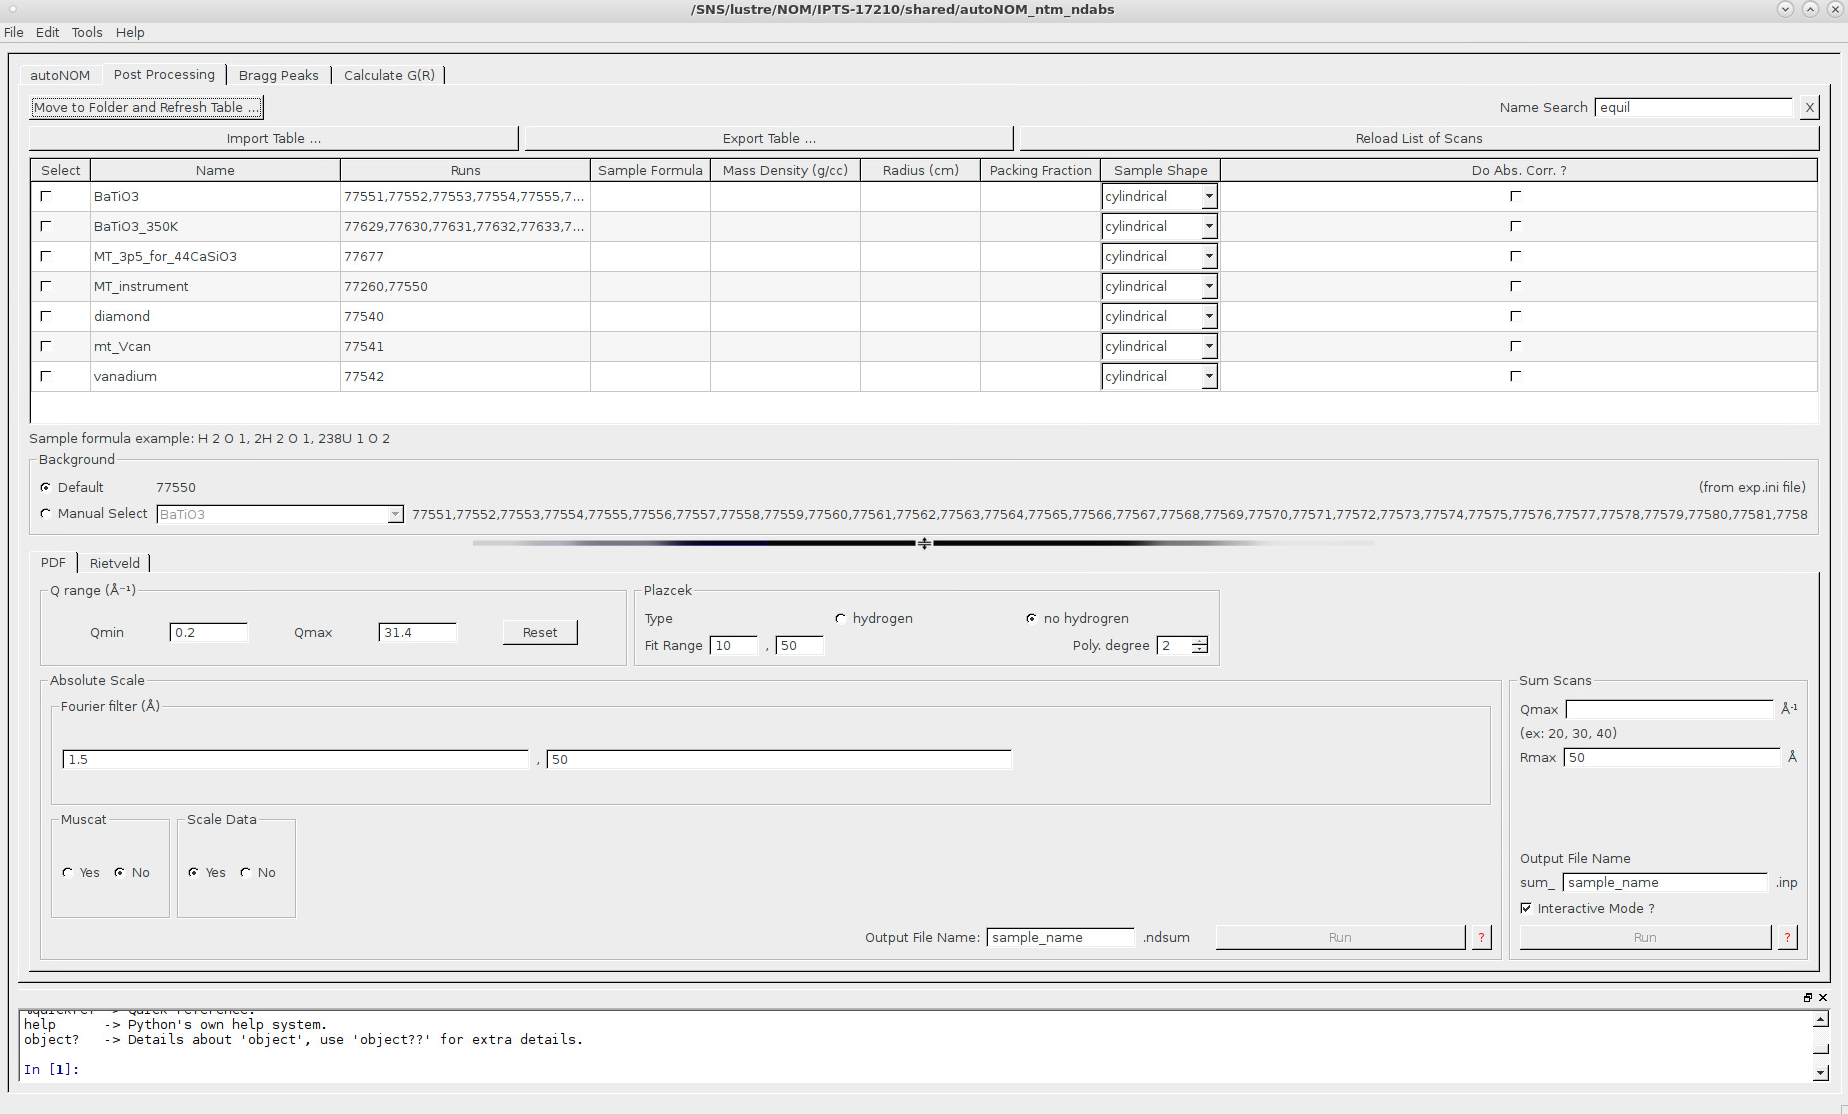
\includegraphics[width=0.9\paperwidth]{graphics/tab2/tab2_populatedTable.png}}

\subsection{Selection of Runs}
\subsection{Selection of Post-Processing}
\subsection{Launch Post-Processing}

\section{Visualize Bragg Diffraction}

As individual runs or post-processed runs are completed, the output files will be placed in their respective directories specified in Table \ref{table_directory_struct}. The diffraction data is found in multiple directories: \fileio{GSAS}, \fileio{fullprof}, \fileio{topas}, and \fileio{rietveld}. Also, the \iptsPrint\fileio{/autoreduce} directory will have diffraction data as well. 

To visualize and plot the Bragg diffraction data, we use the \guicmd{Bragg Peaks} tab shown below and we view the files located in the \fileio{GSAS} directory: 

\noindent\makebox[\textwidth]{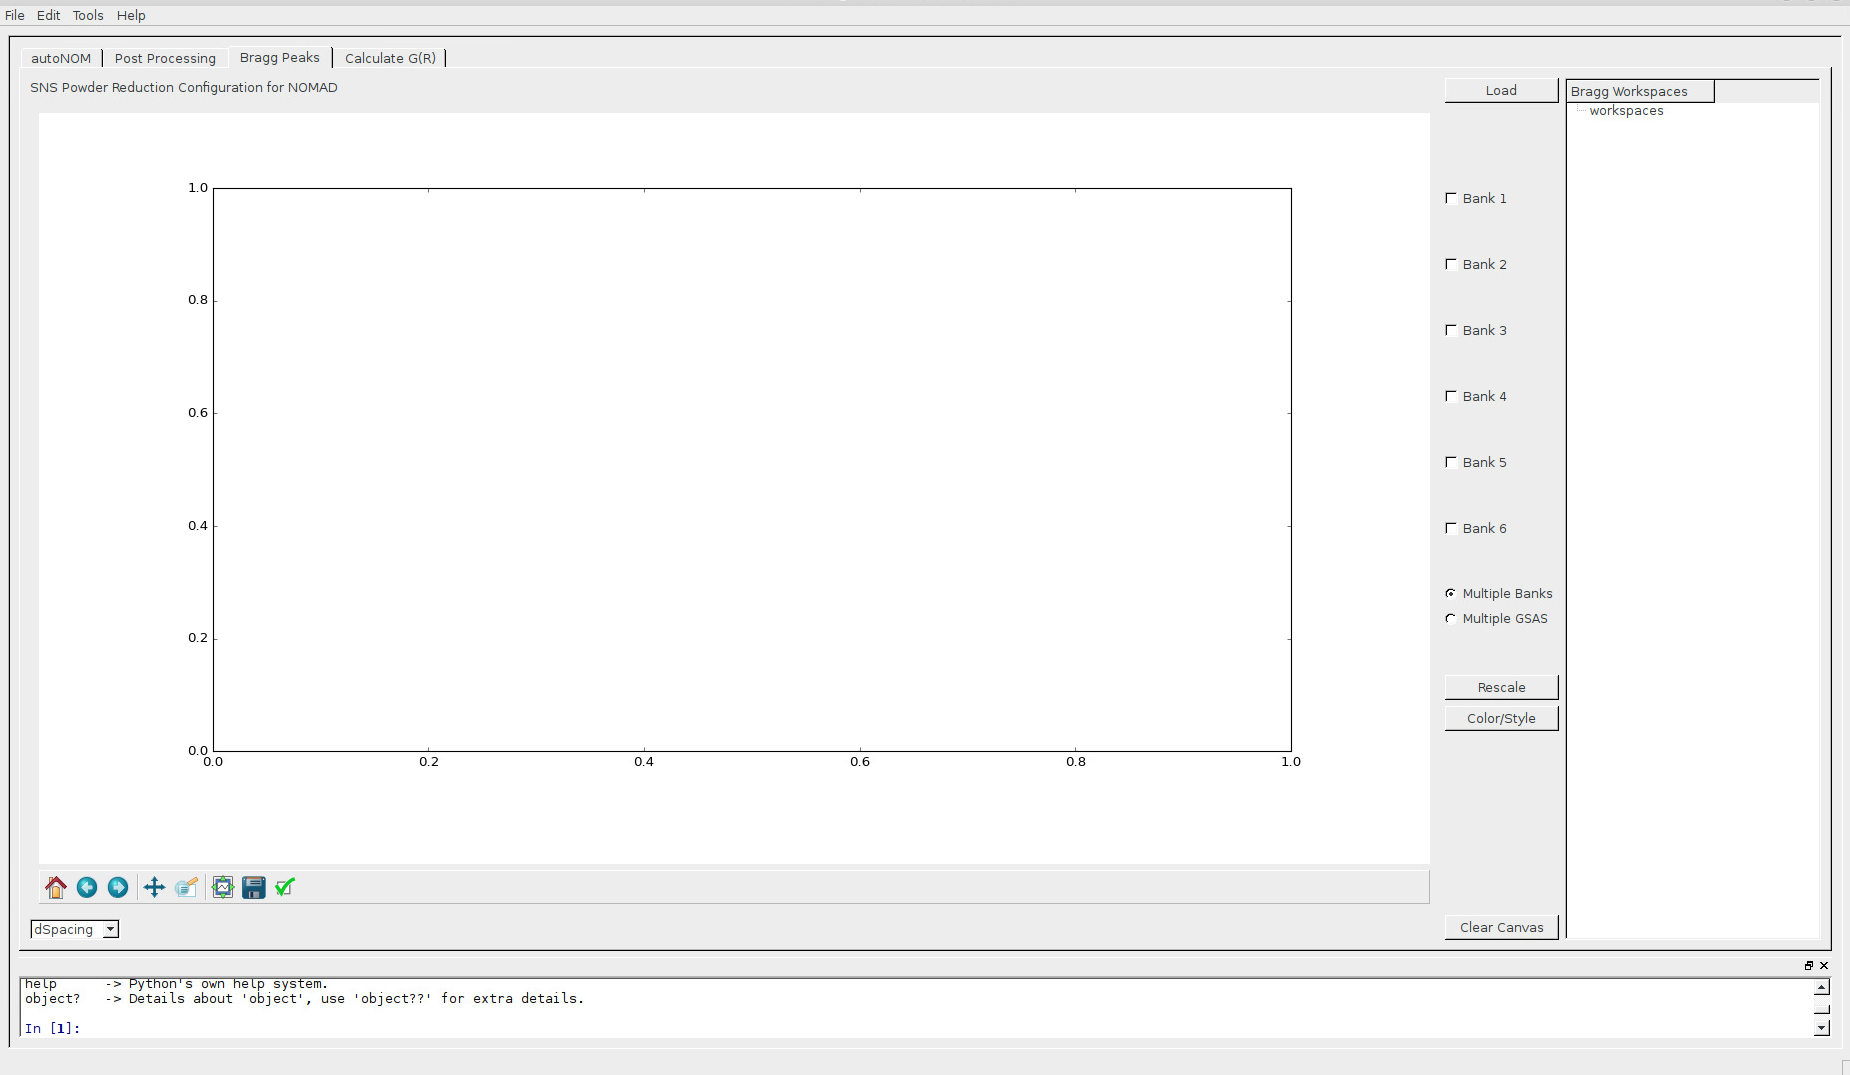
\includegraphics[width=0.9\paperwidth]{graphics/tab3/tab3.png}}

\subsection{Load Bragg data}

First we need to load in diffraction data. Go to the top right and press the \guicmd{Load} button. You should be presented with a file dialog similar to the one below:

\noindent\makebox[\textwidth]{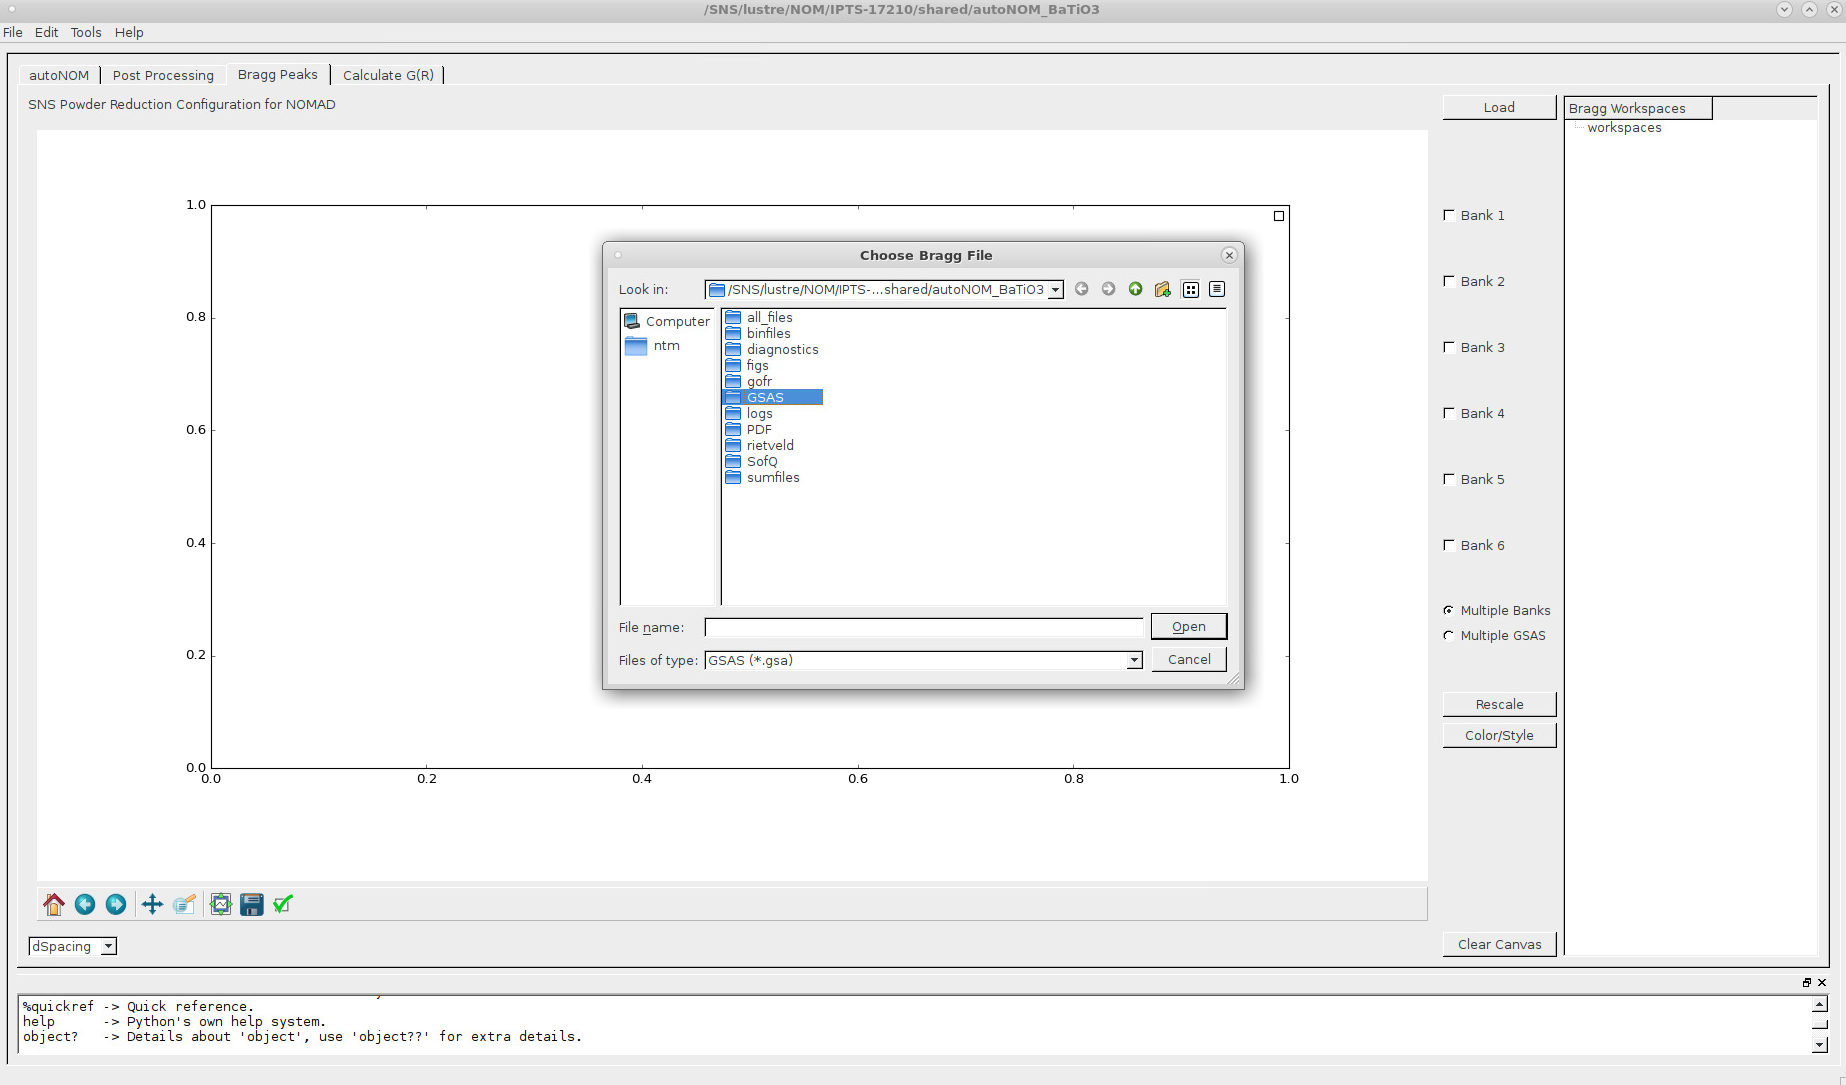
\includegraphics[width=0.9\paperwidth]{graphics/tab3/tab3_loadFiles.png}}

Double-click the \fileio{GSAS} diretory to see the files that are available. When you press \guicmd{Load}, you may actually start in the \fileio{GSAS} directory as well. From here, you can select individual runs, labeled as \fileio{NOM<run number>tof.gsa} or you can select post-processed runs such as summed files, labeled as \fileio{NOM\_<given title>.gsa}.  An example is displayed below:

\noindent\makebox[\textwidth]{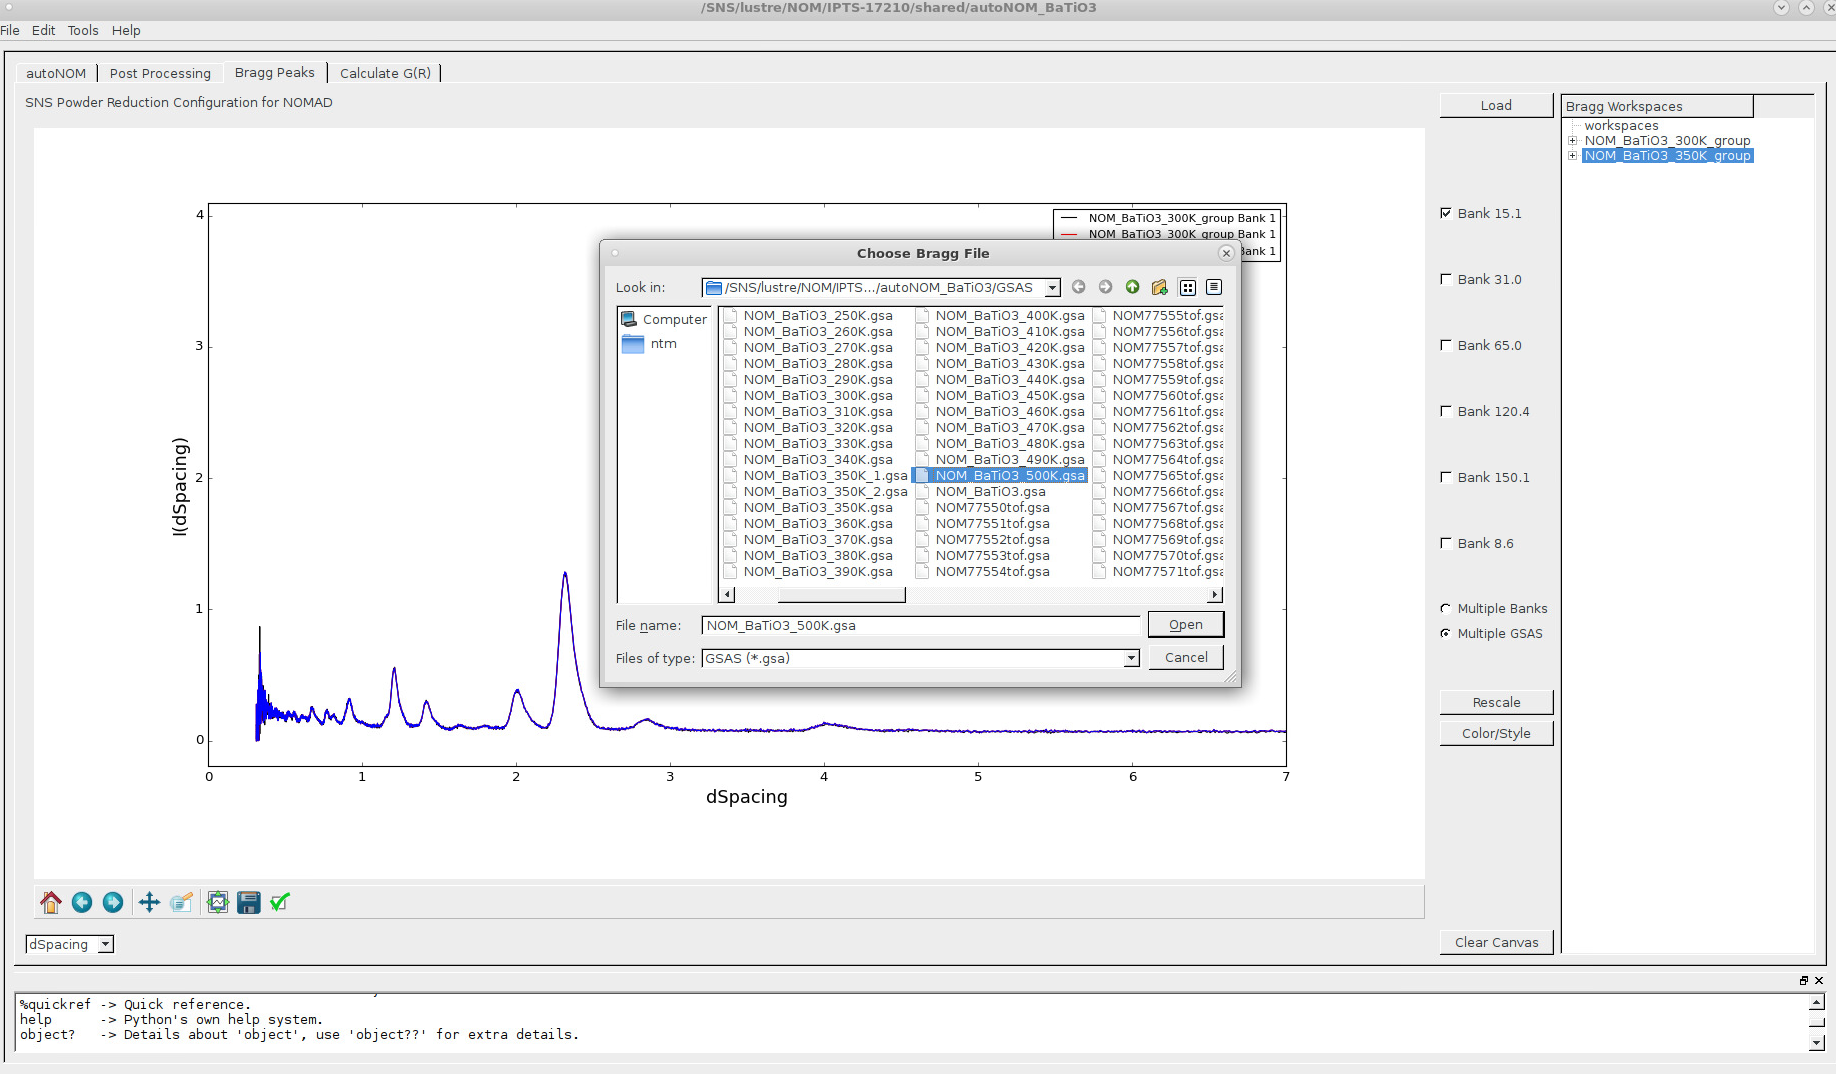
\includegraphics[width=0.9\paperwidth]{graphics/tab3/tab3_loadFiles_showIndiviuals.png}}

You can also select multiple individual runs while holding the \cmd{Ctrl} key or you can select a span of runs by holding the \cmd{Shift} key while selecting the runs. Once the runs are selected, press the \guicmd{Open} button. 

Below we show where we have loaded the summed run for 300K. 

\noindent\makebox[\textwidth]{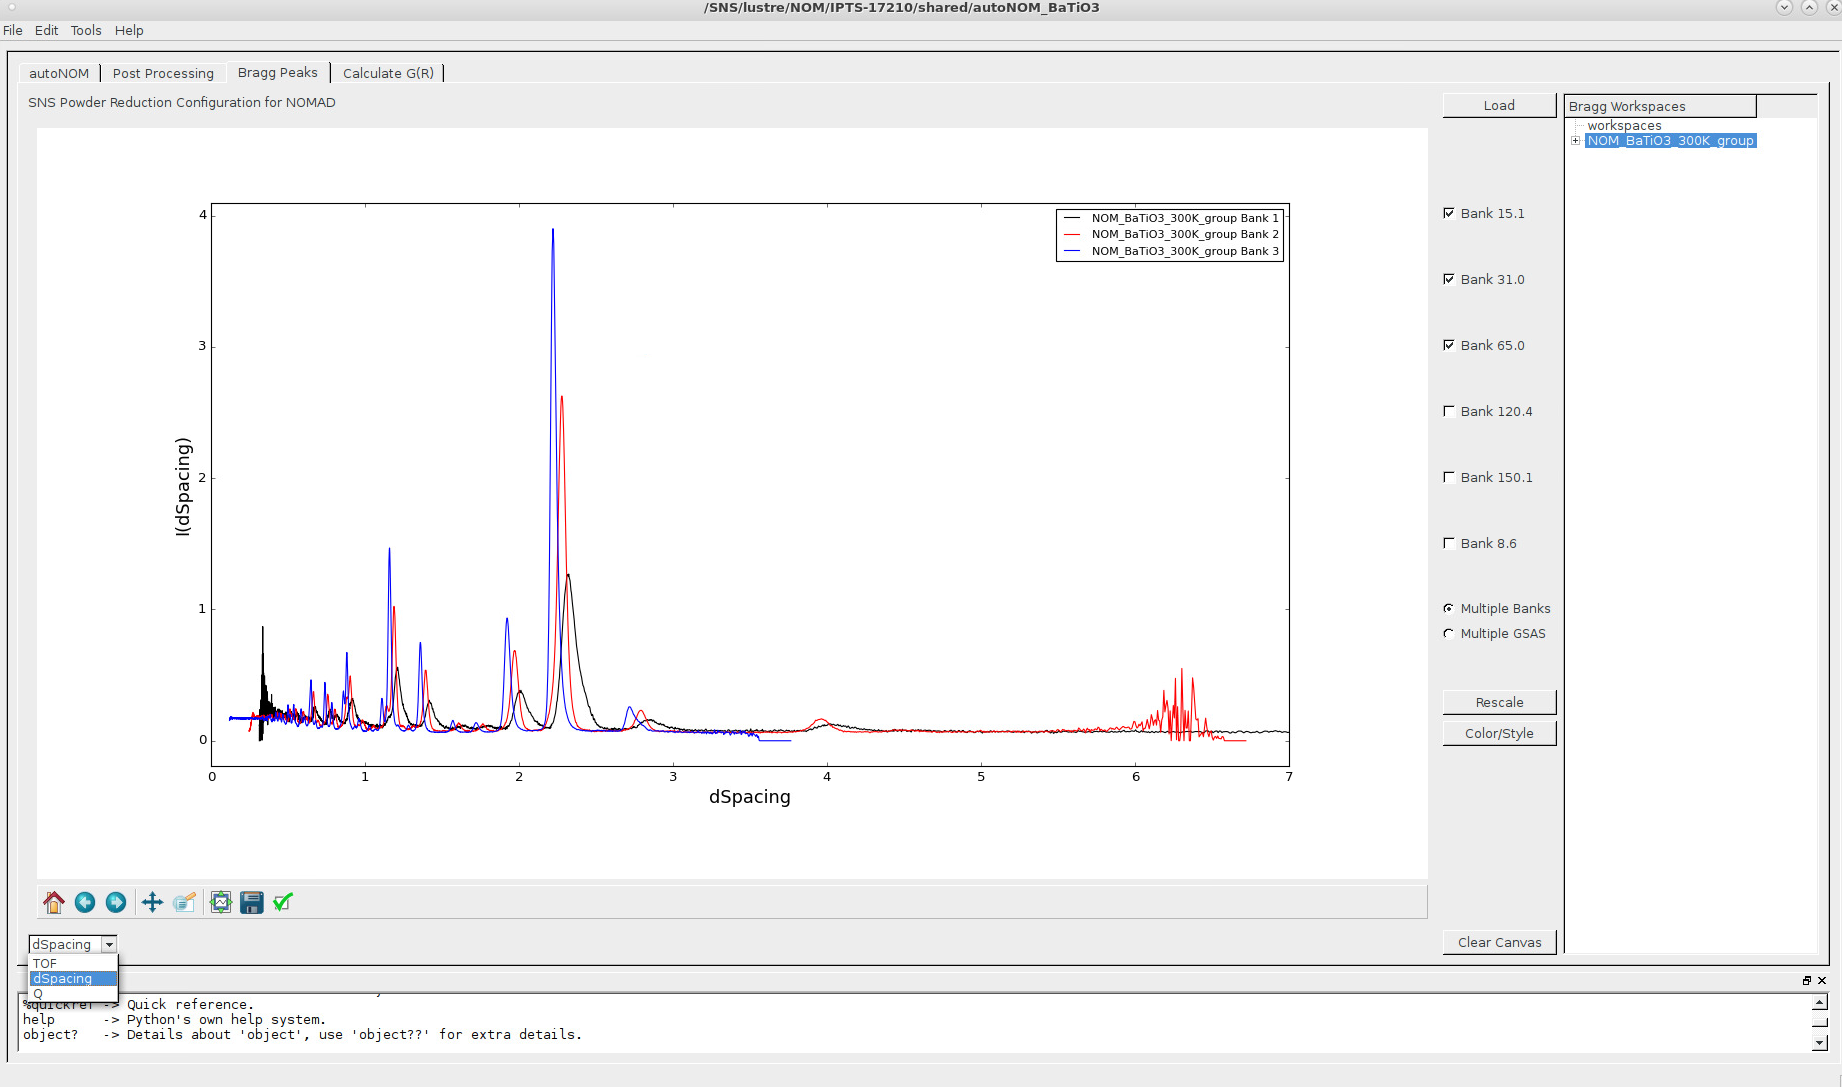
\includegraphics[width=0.9\paperwidth]{graphics/tab3/tab3_multipleBanks.png}} \label{fig_multiBraggBanks}

\subsection{Adjust Graphs}

This tab has two modes to view the diffraction data from the banks: \guicmd{Multiple Banks} and \guicmd{Multiple GSAS}. 

\begin{itemize}

\item \guicmd{Multiple Banks}: In this mode, we can view diffraction data from different banks of the same run. We can select the banks to display on the right-hand side. We can select multiple different banks in this mode.

\item \guicmd{Multiple GSAS}: In this mode, we can view diffraction data from different runs for a single bank. We can select the bank to display on the right-hand side. We can select only one bank at a time in this mode.

\end{itemize}

In Figure \ref{fig_multiBraggBanks}, we are in \guicmd{Multiple Banks} mode and have three of the banks selected. When we load in more than one dataset, we can use \guicmd{Multiple GSAS} mode. Below, we show where we have loaded in the 300K, 350K, and 500K data sets and have selected the 31.0 degree bank to view the data:

\noindent\makebox[\textwidth]{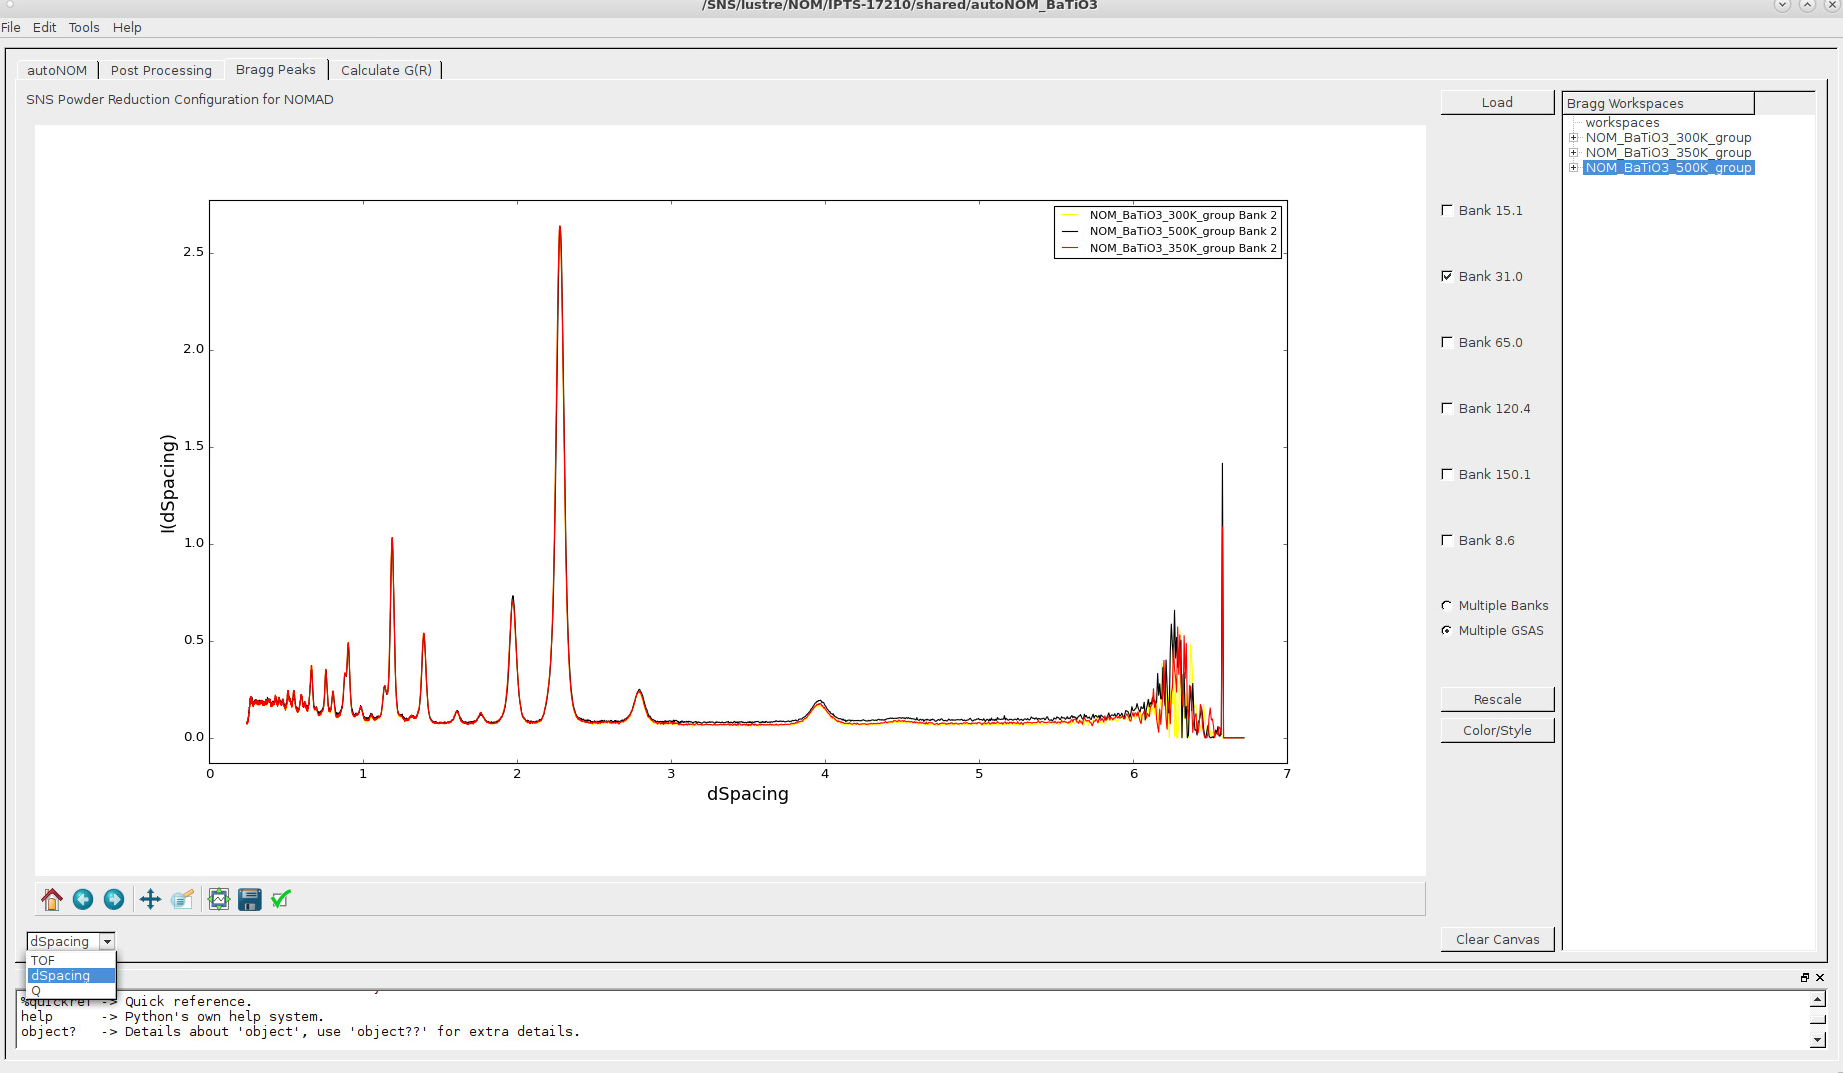
\includegraphics[width=0.9\paperwidth]{graphics/tab3/tab3_multipleGSAS.png}} \label{fig_multiBraggBanks}

Under the bank and mode selection, we have the \guicmd{Rescale} and \guicmd{Color/Style} buttons. The \guicmd{Rescale} button can be used to rescale the frame to better fit the data if the y-axis spans too far or not enought to capture the data. The \guicmd{Color/Style} button can be used to change the display of the data in the plot. After pressing the \guicmd{Color/Style} button, we are presented with a file dialog box. We can select the workspace from the drop-down list we would like to change, shown below, and can change the color of the curve, add markers, and select the fill and edge color of the markers from the other drop-downs: 

\noindent\makebox[\textwidth]{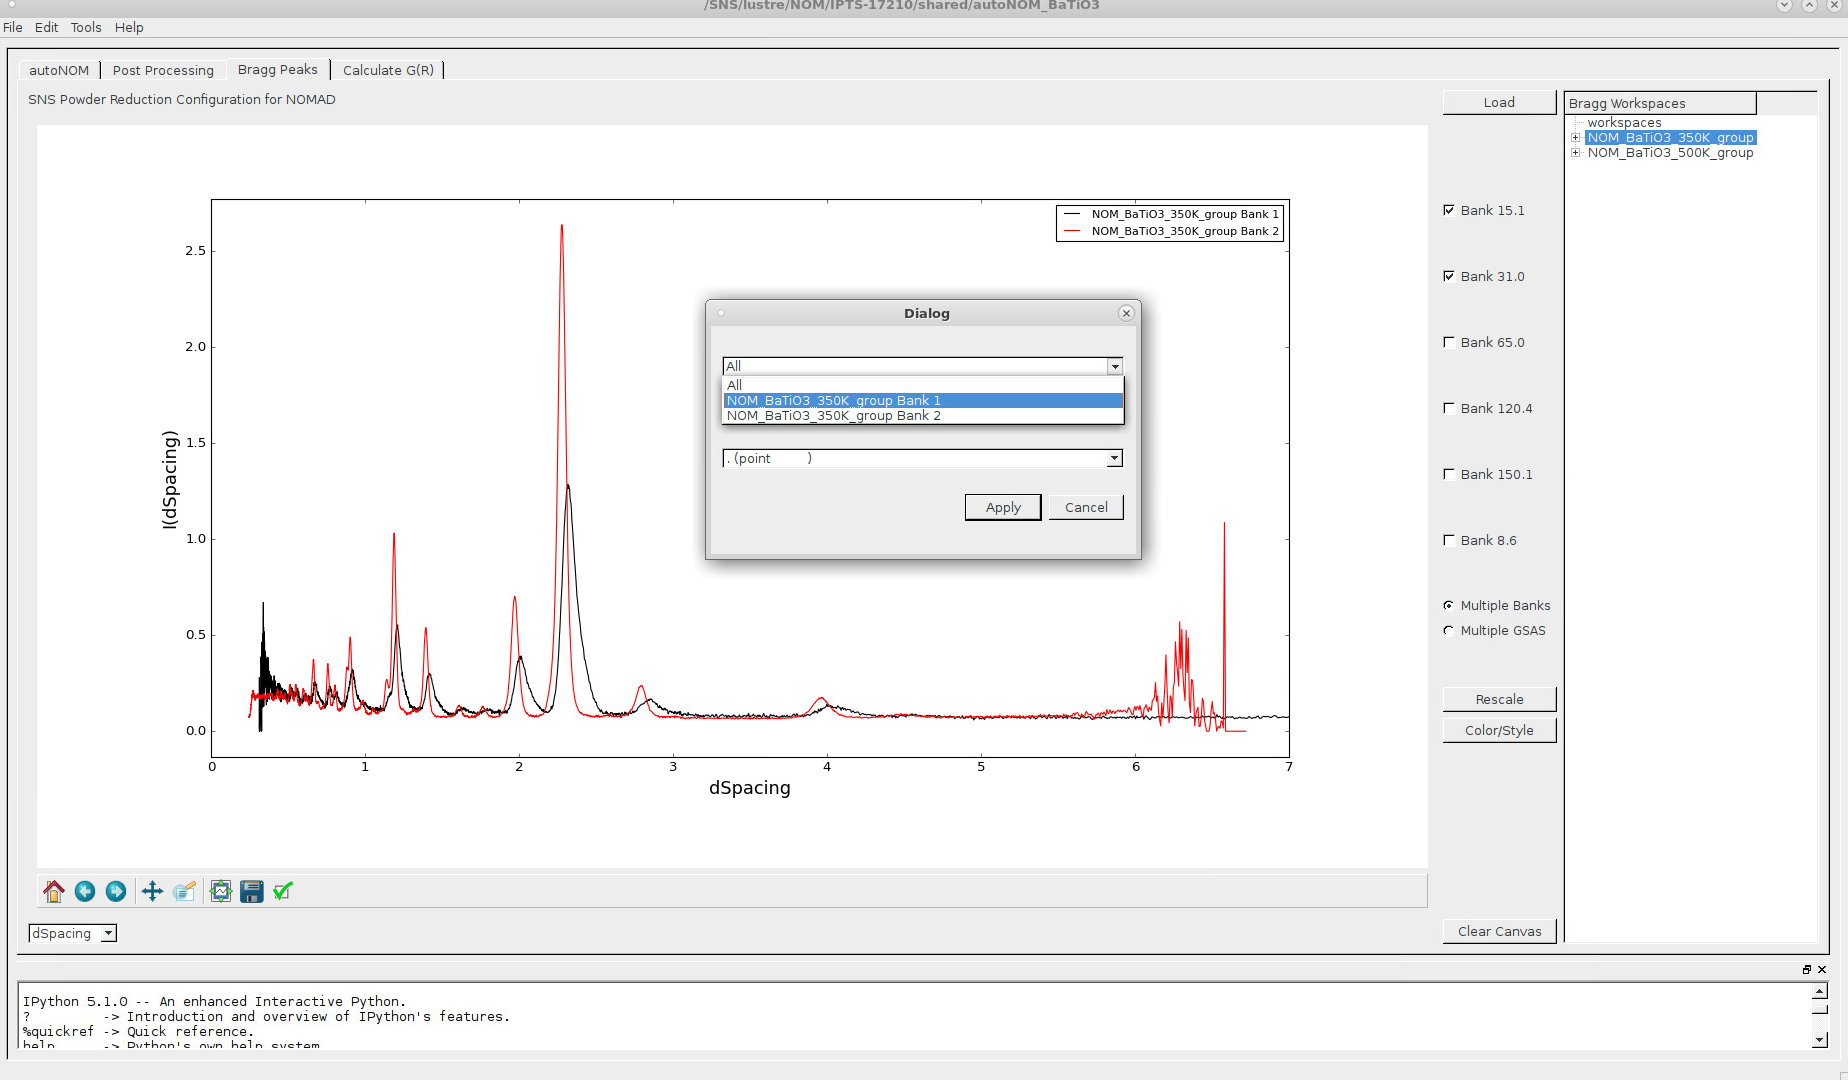
\includegraphics[width=0.9\paperwidth]{graphics/tab3/tab3_colorStyle.png}} 

Under the \guicmd{Rescale} and \guicmd{Color/Style}, we have the \guicmd{Clear Canvas} button. This can be used to quickly clear the plot of all datasets and begin again.

You will also notice in the bottom left of the tab space  that we can change the x-axis that we display the graph in. The choices are: \guicmd{TOF} for time-of-flight, \guicmd{dSpacing} for d-spacing (the default), and \guicmd{Q} for momentum transfer. The graph will change accordingly. 

For each of the datasets that have been loaded, we have a \guicmd{Bragg Workspaces} tree on the far right side. If you right-click on any of the workspaces, you will see the following options, demonstrated below:

\noindent\makebox[\textwidth]{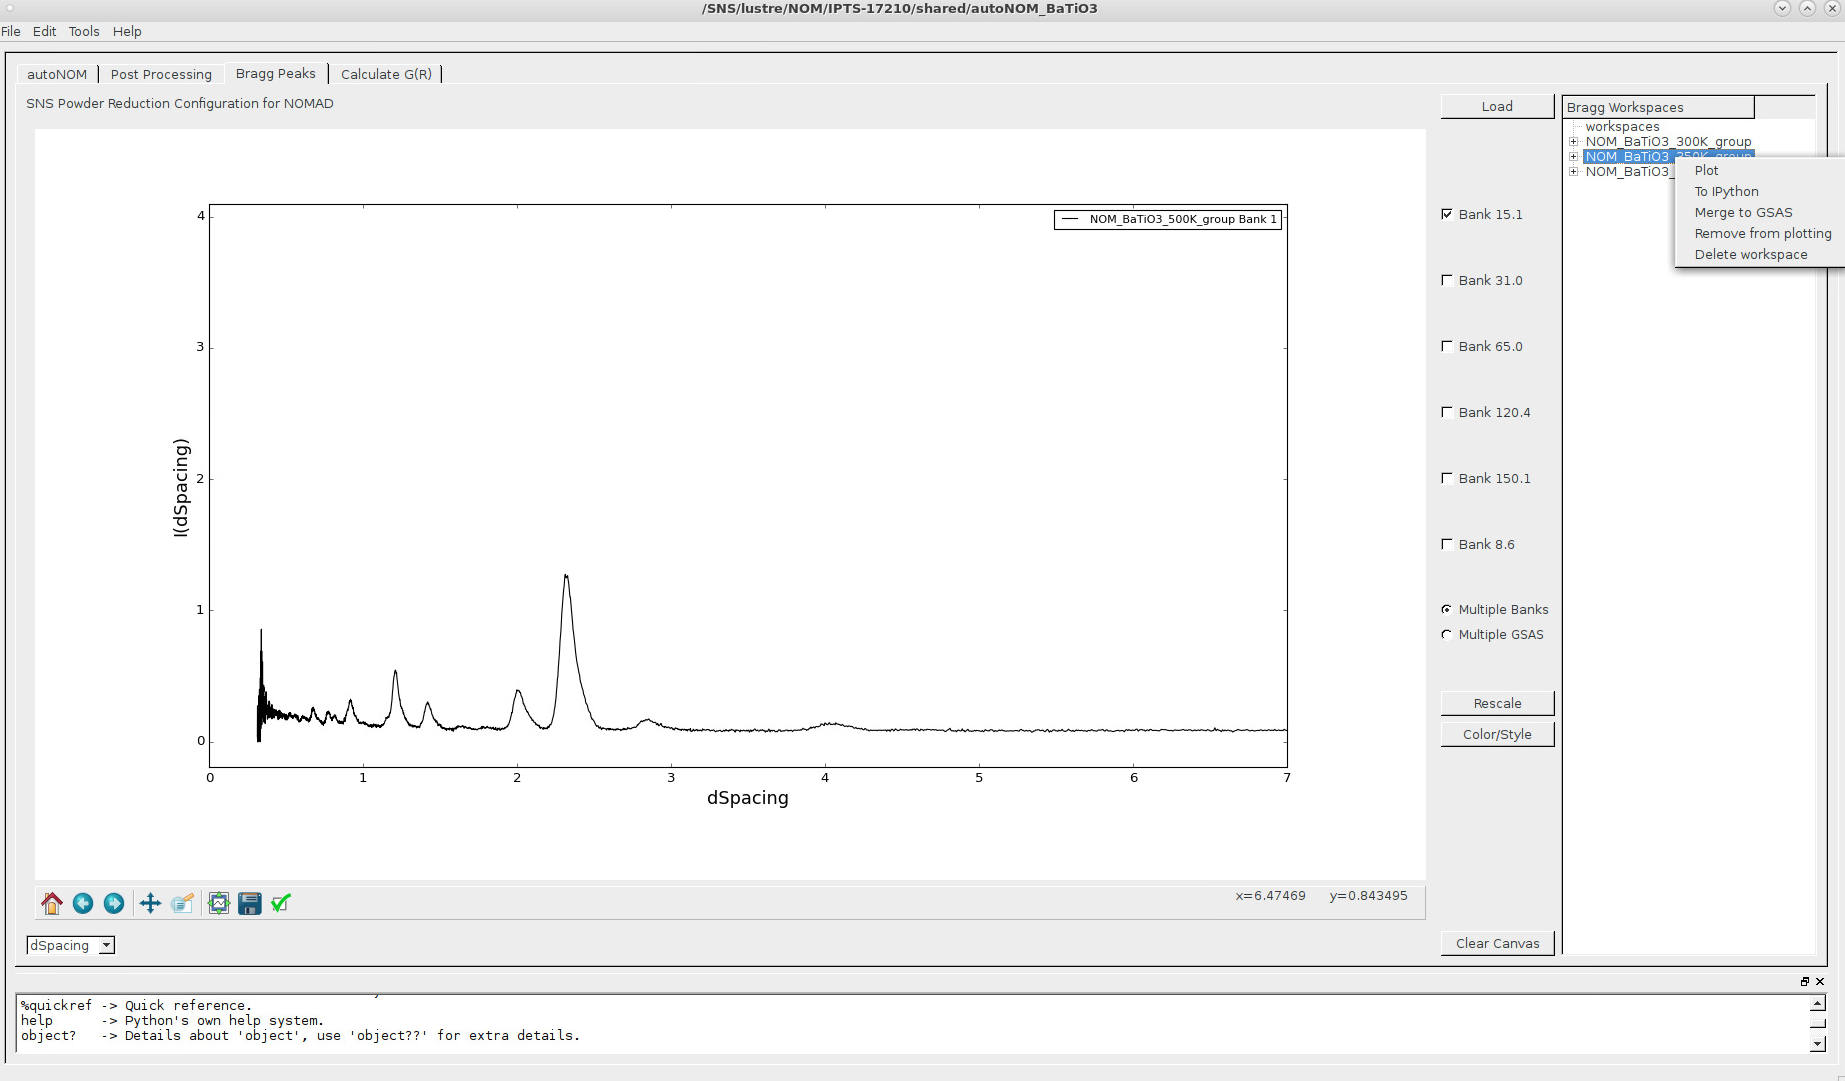
\includegraphics[width=0.9\paperwidth]{graphics/tab3/tab3_rightClick.png}} 

From the options, you can do the following:

\begin{itemize}

\item \guicmd{Plot}: Plot the selected workspace on the graph area.

\item \guicmd{To IPython}: Transfer the workspace to the IPython command line dock at the bottom. Here, you can script changes to the workspace and output a new workspace. If clicked, you will have something similar to what is shown below:

\noindent\makebox[\textwidth]{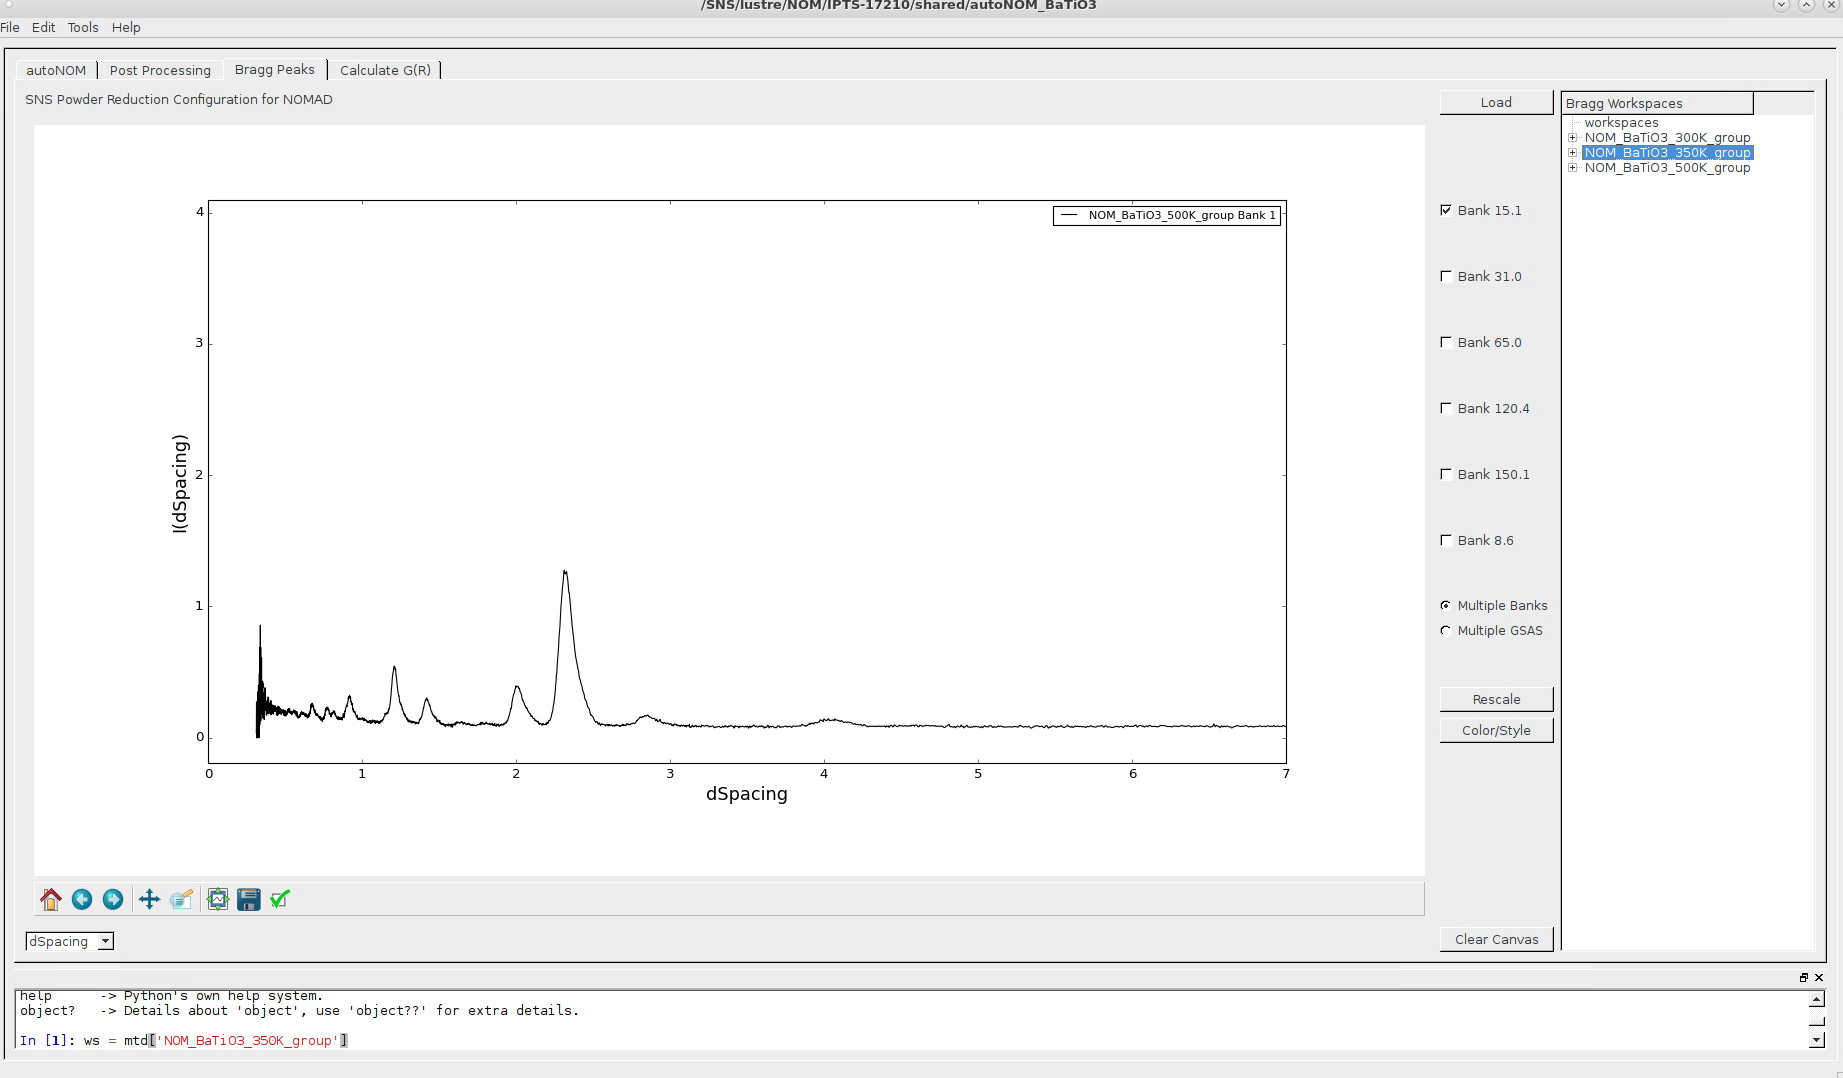
\includegraphics[width=0.8\paperwidth]{graphics/tab3/tab3_rightClick_toIPython.png}}

You can "undock" the IPython command line dock by pressing the double-window icon in the top right of the dock, shown below:

\noindent\makebox[\textwidth]{
\includegraphics[width=0.1\paperwidth]{graphics/tab3/tab3_rightClick_icon.png}} 

This will allow you to expand and contract the IPython command line dock. At anytime, you can redock by pressing the same double-window icon in the top right of the dock:

\noindent\makebox[\textwidth]{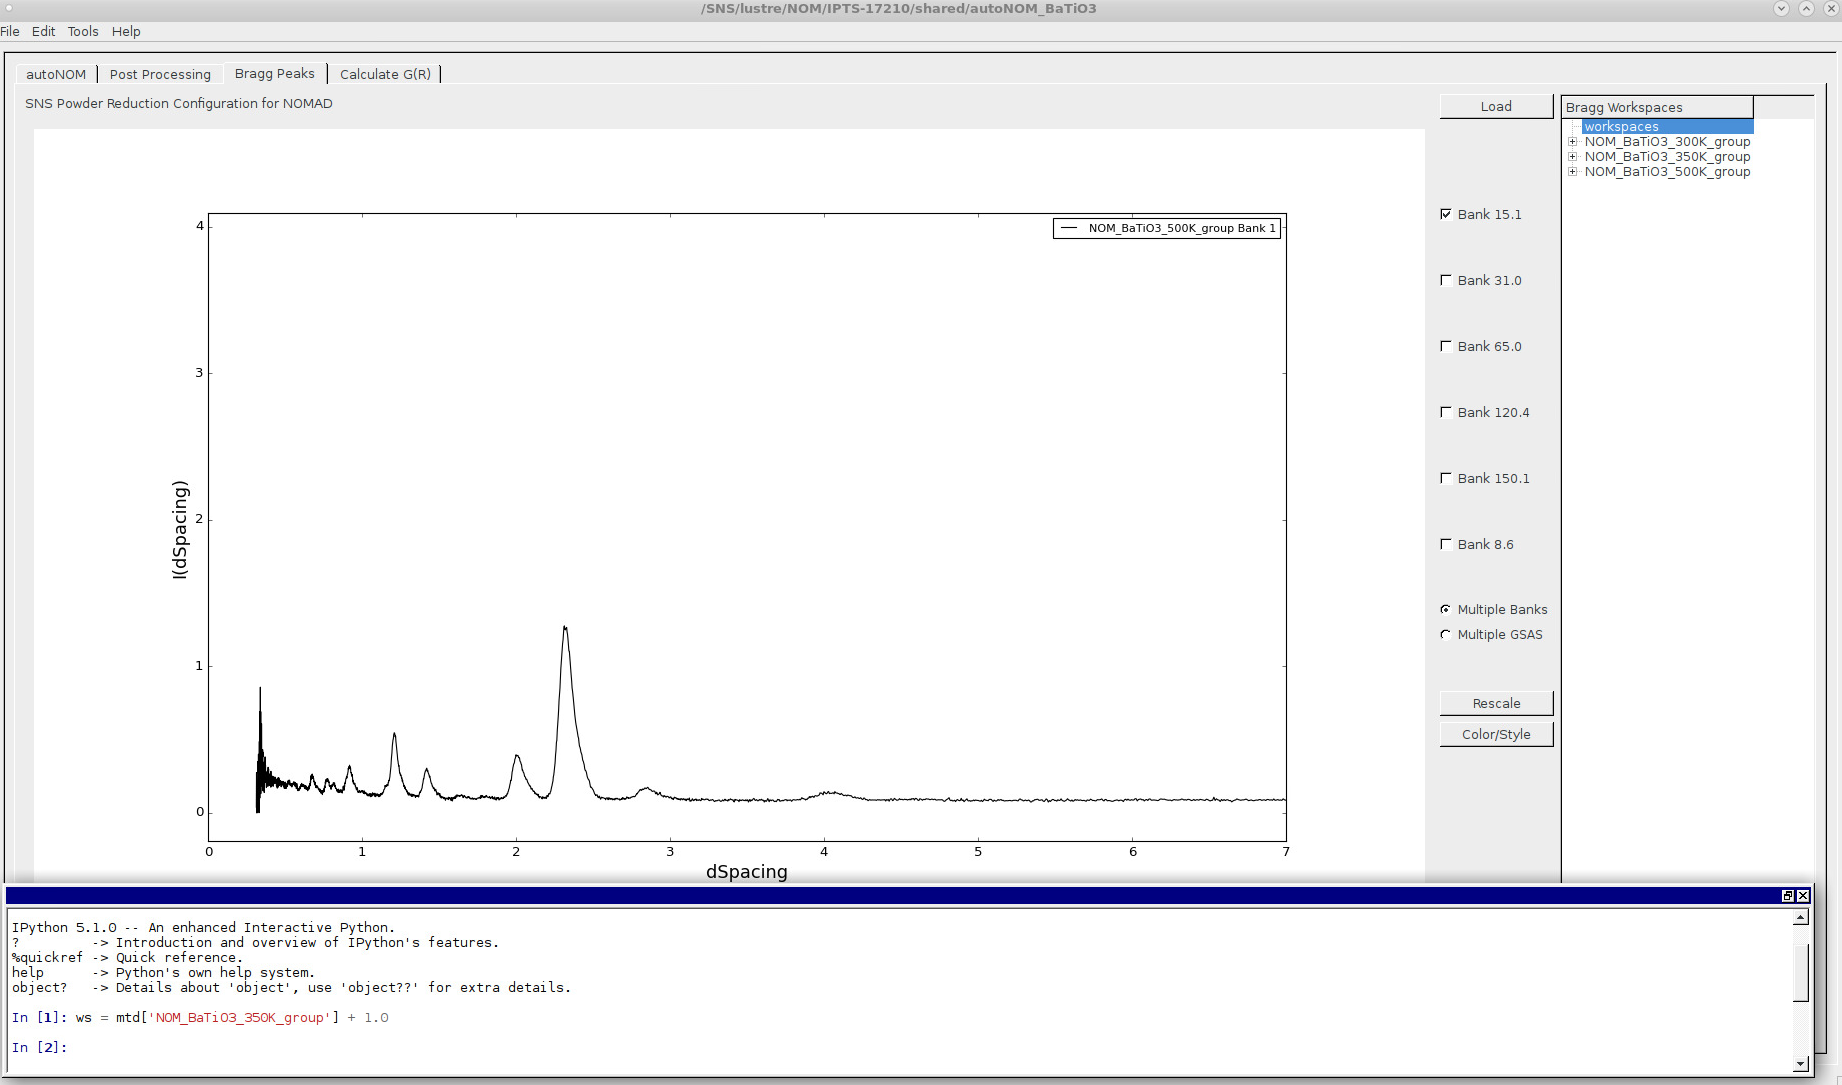
\includegraphics[width=0.8\paperwidth]{graphics/tab3/tab3_rightClick_toIPython_unDock.png}}

\item \guicmd{Merge to GSAS}: Will give a merged GSAS output file of the banks.
\item \guicmd{Remove from plotting}: Removes dataset from the plot.
\item \guicmd{Delete workspace}: Deletes the dataset from the \guicmd{Bragg Workspaces} tree.

\end{itemize}

To change the legend, in case it is in the way or masking data, you can right-click inside any of the plot areas and either reduce the font of the text, increase the font of the text, or hide the legend all together.




\section{Visualize S(Q) and G(r)}

As individual runs or post-processed runs are completed, the output files will be placed in their respective directories specified in Table \ref{table_directory_struct}. The S(Q) data is found in the \fileio{SofQ} directory and the real-space data is found in the \fileio{gofr} and \fileio{PDF}. 

To visualize and plot both sets of of data (reciprocal-space and real-space), we use the \guicmd{Calculate G(r)} tab shown below: 

\noindent\makebox[\textwidth]{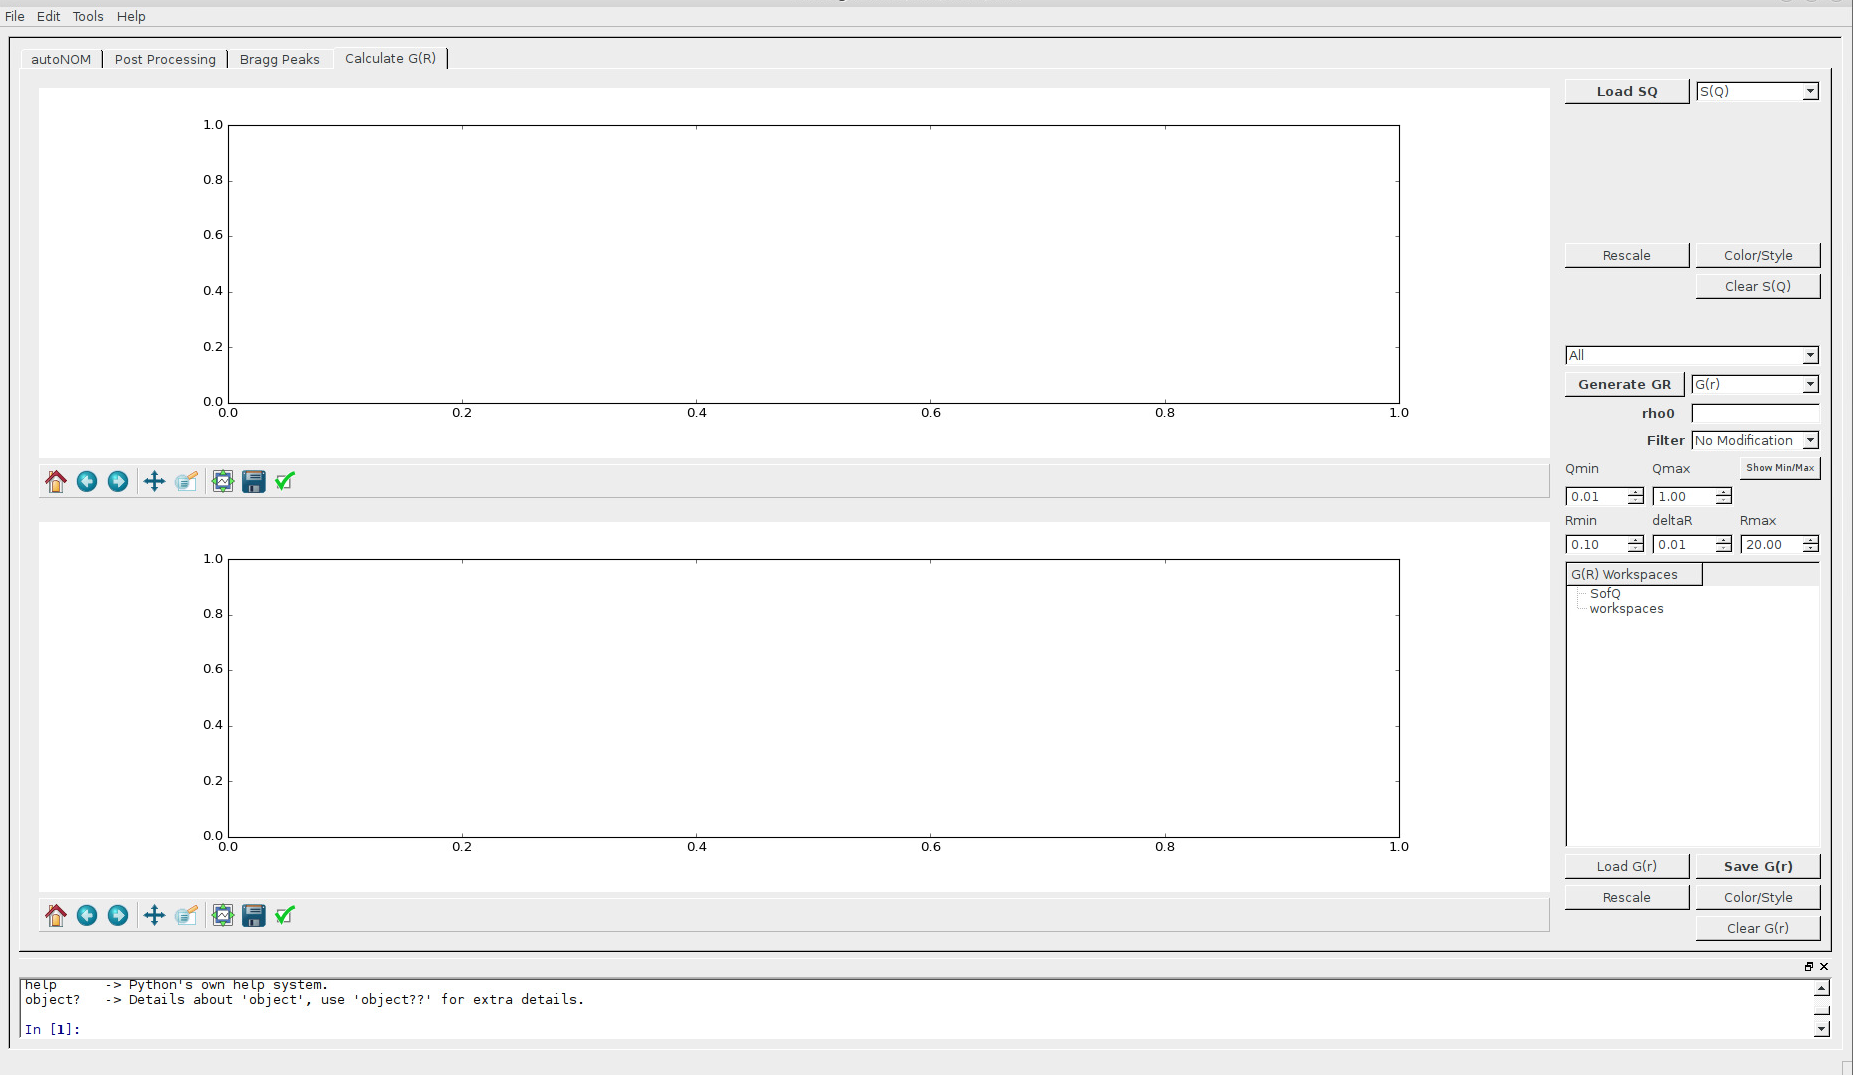
\includegraphics[width=0.9\paperwidth]{graphics/tab4/tab4.png}}

A note on how the two plots work: When S(Q) data is loaded in, the Fourier transform is calculated automatically and the corresponding G(r) is displayed in the corresponding plot. Thus, ADDIE allows one to simultaneously view both the S(Q) and corresponding G(r) and also adjust and refine both datasets in an "on-the-fly" manner.

\subsection{Load S(Q) data}

First load in S(Q) datasests. Go to the top right and press the \guicmd{Load SQ} button. You should be presented with a file dialog similar to the one below:

\noindent\makebox[\textwidth]{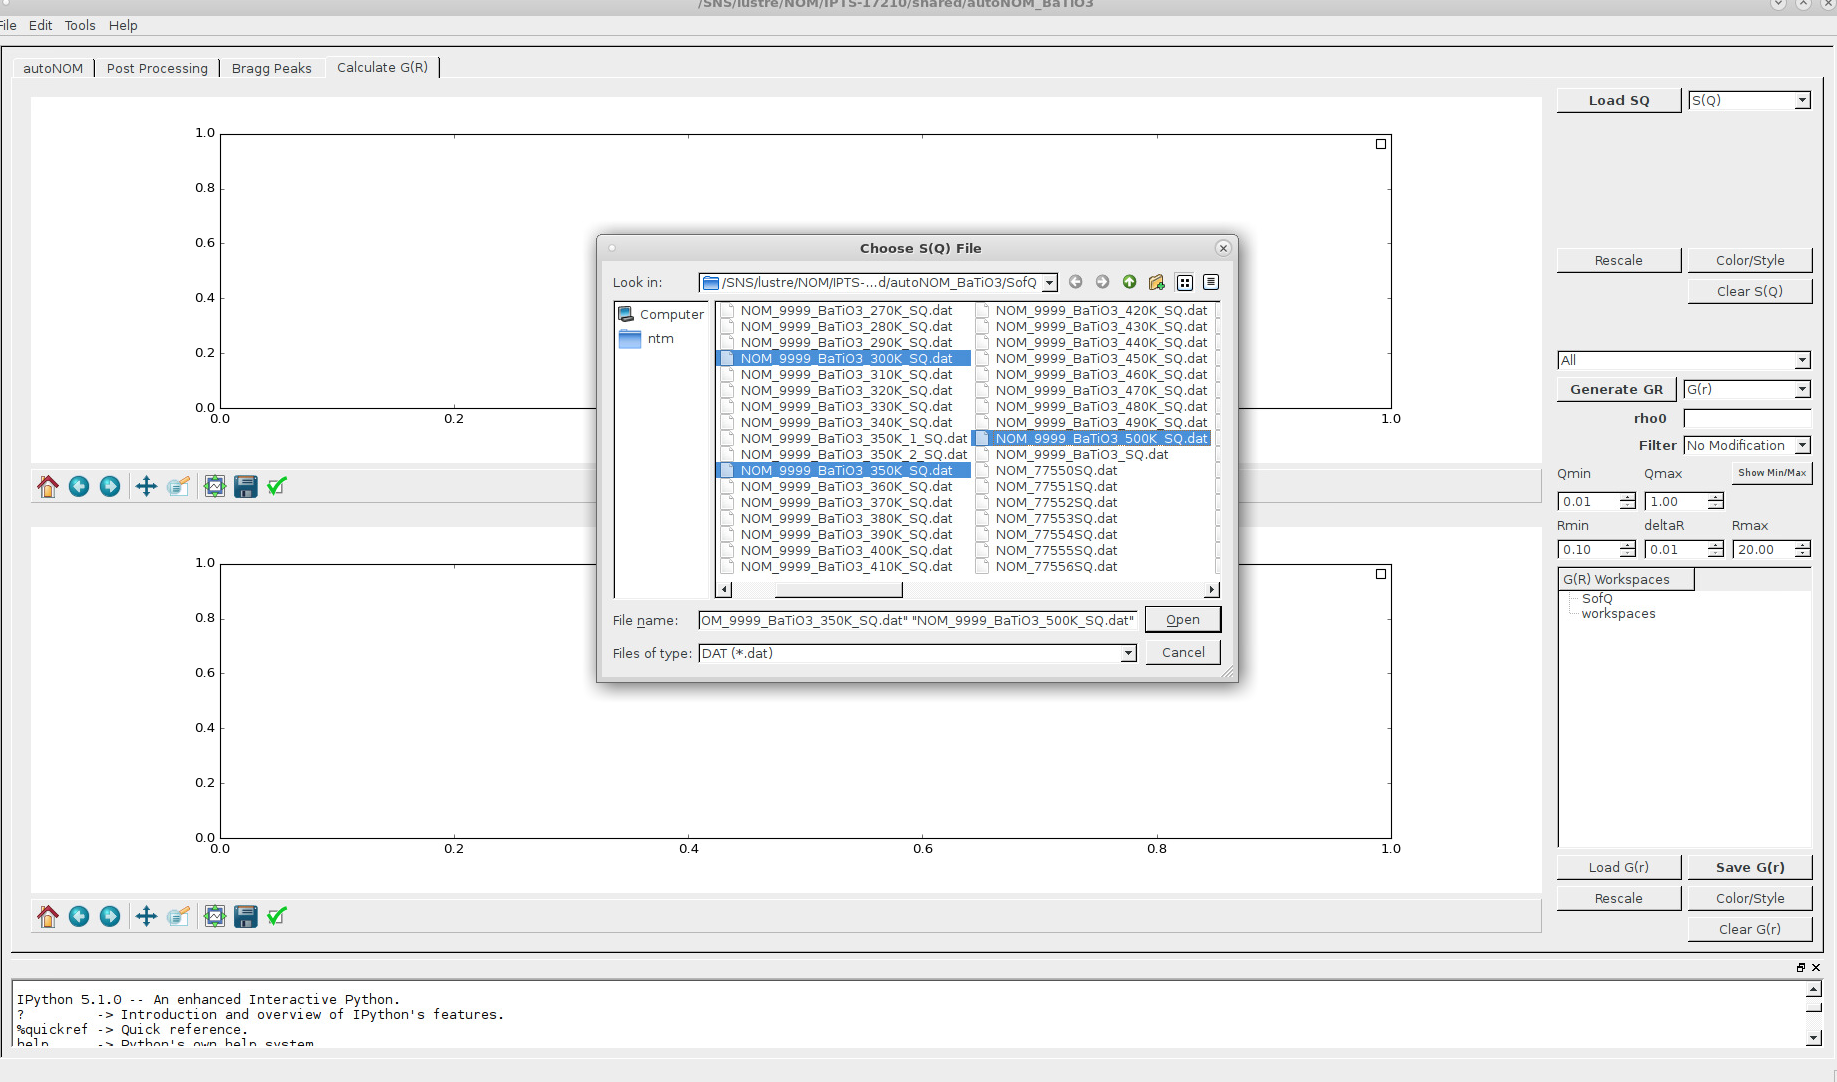
\includegraphics[width=0.9\paperwidth]{graphics/tab4/tab4_loadSQ.png}}

If you are not in the \fileio{SofQ} directory, double-click the \fileio{SofQ} diretory to see the files that are available.  From here, you can select individual runs, labeled as \fileio{NOM\_<run number>SQ.dat} or you can select post-processed runs such as summed files, labeled as \fileio{NOM\_9999\_<given title>\_SQ.dat}.

You can also select multiple individual runs while holding the \cmd{Ctrl} key or you can select a span of runs by holding the \cmd{Shift} key while selecting the runs. Once the runs are selected, press the \guicmd{Open} button. For our example above, we get the following displayed:

\noindent\makebox[\textwidth]{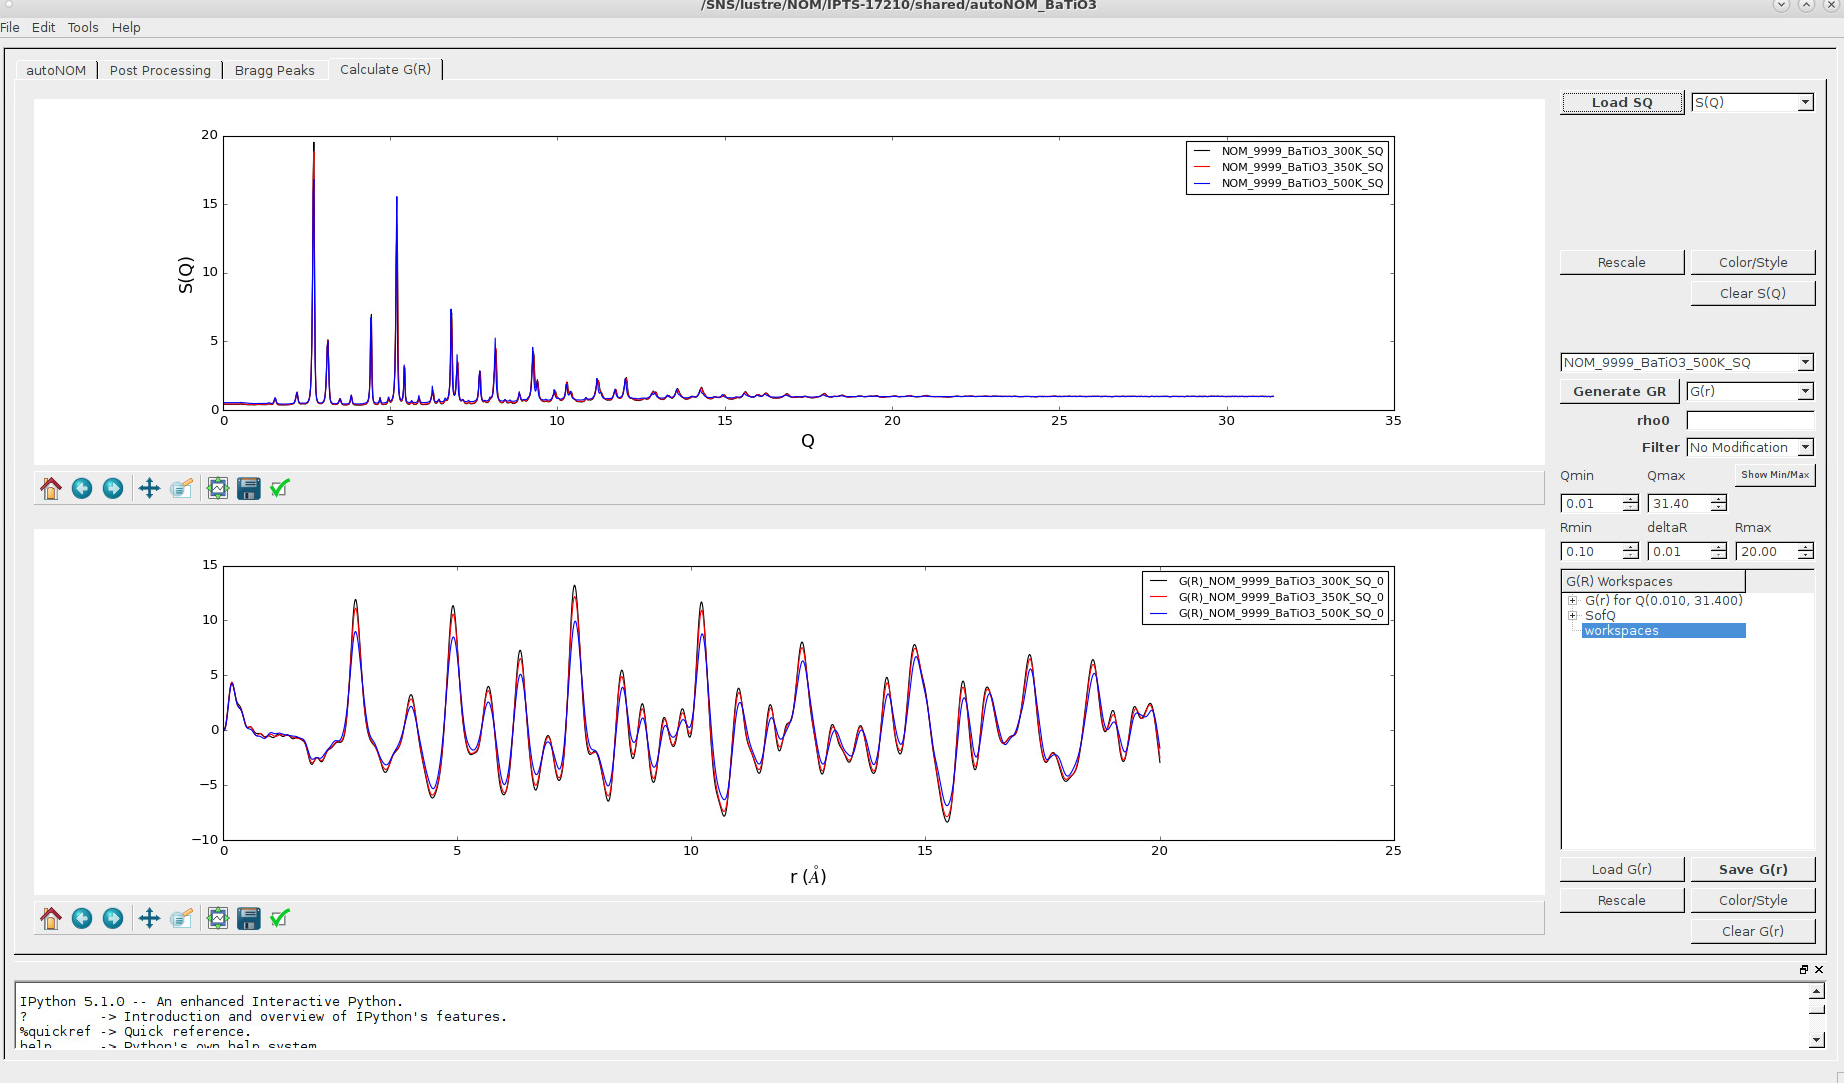
\includegraphics[width=0.9\paperwidth]{graphics/tab4/tab4_loadSQ_afterLoaded.png}}

We can see all three datasets were loaded and the Fourier transform data is displayed as well, based on the current options set for the transform, described more below. 

\subsection{Adjust S(Q) graphs}

On the top right, next to the \guicmd{Load SQ} button, we can change the x-axis of the reciprocal-space plot. We can choose from \guicmd{S(Q)}, \guicmd{S(Q)-1}, and \guicmd{Q[S(Q)-1]}, shown below:

\noindent\makebox[\textwidth]{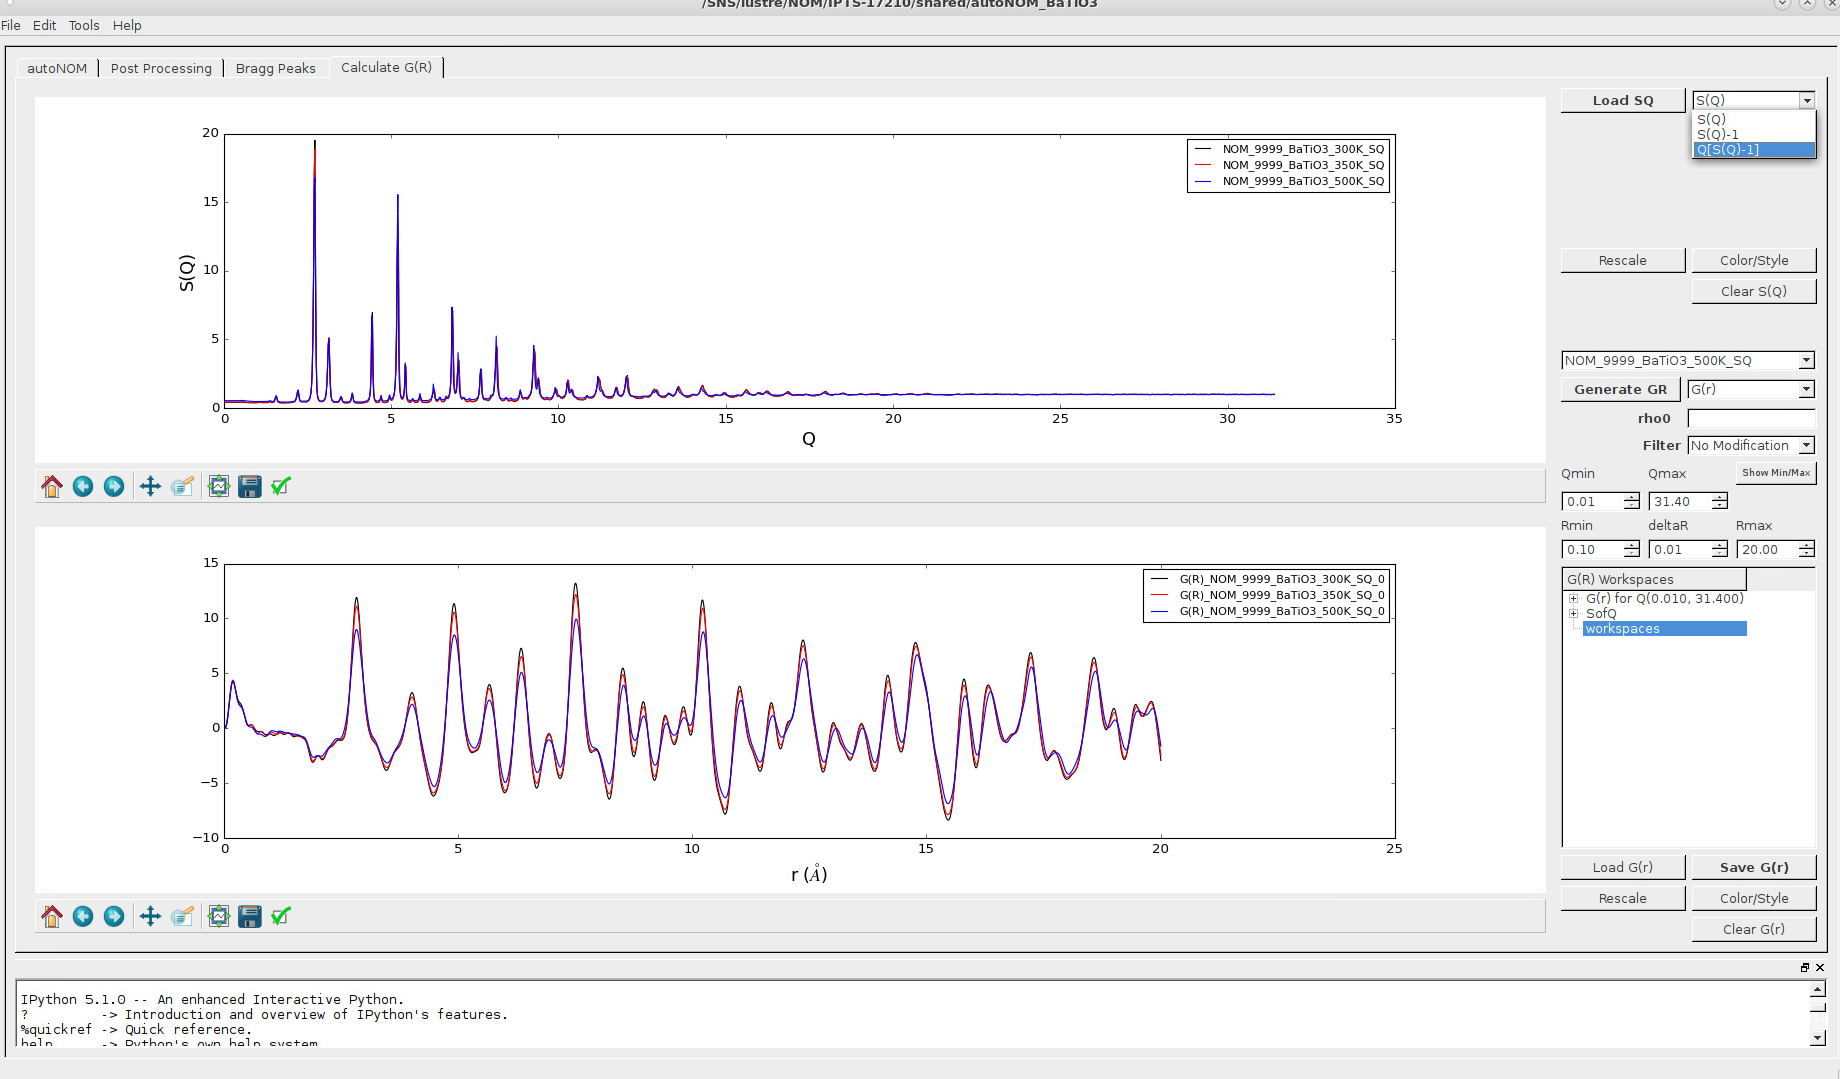
\includegraphics[width=0.9\paperwidth]{graphics/tab4/tab4_populatedGraph_sofqXaxisDropDown.png}}

Selecting the \guicmd{Q[S(Q)-1]} option will produce a plot view like the one below:

\noindent\makebox[\textwidth]{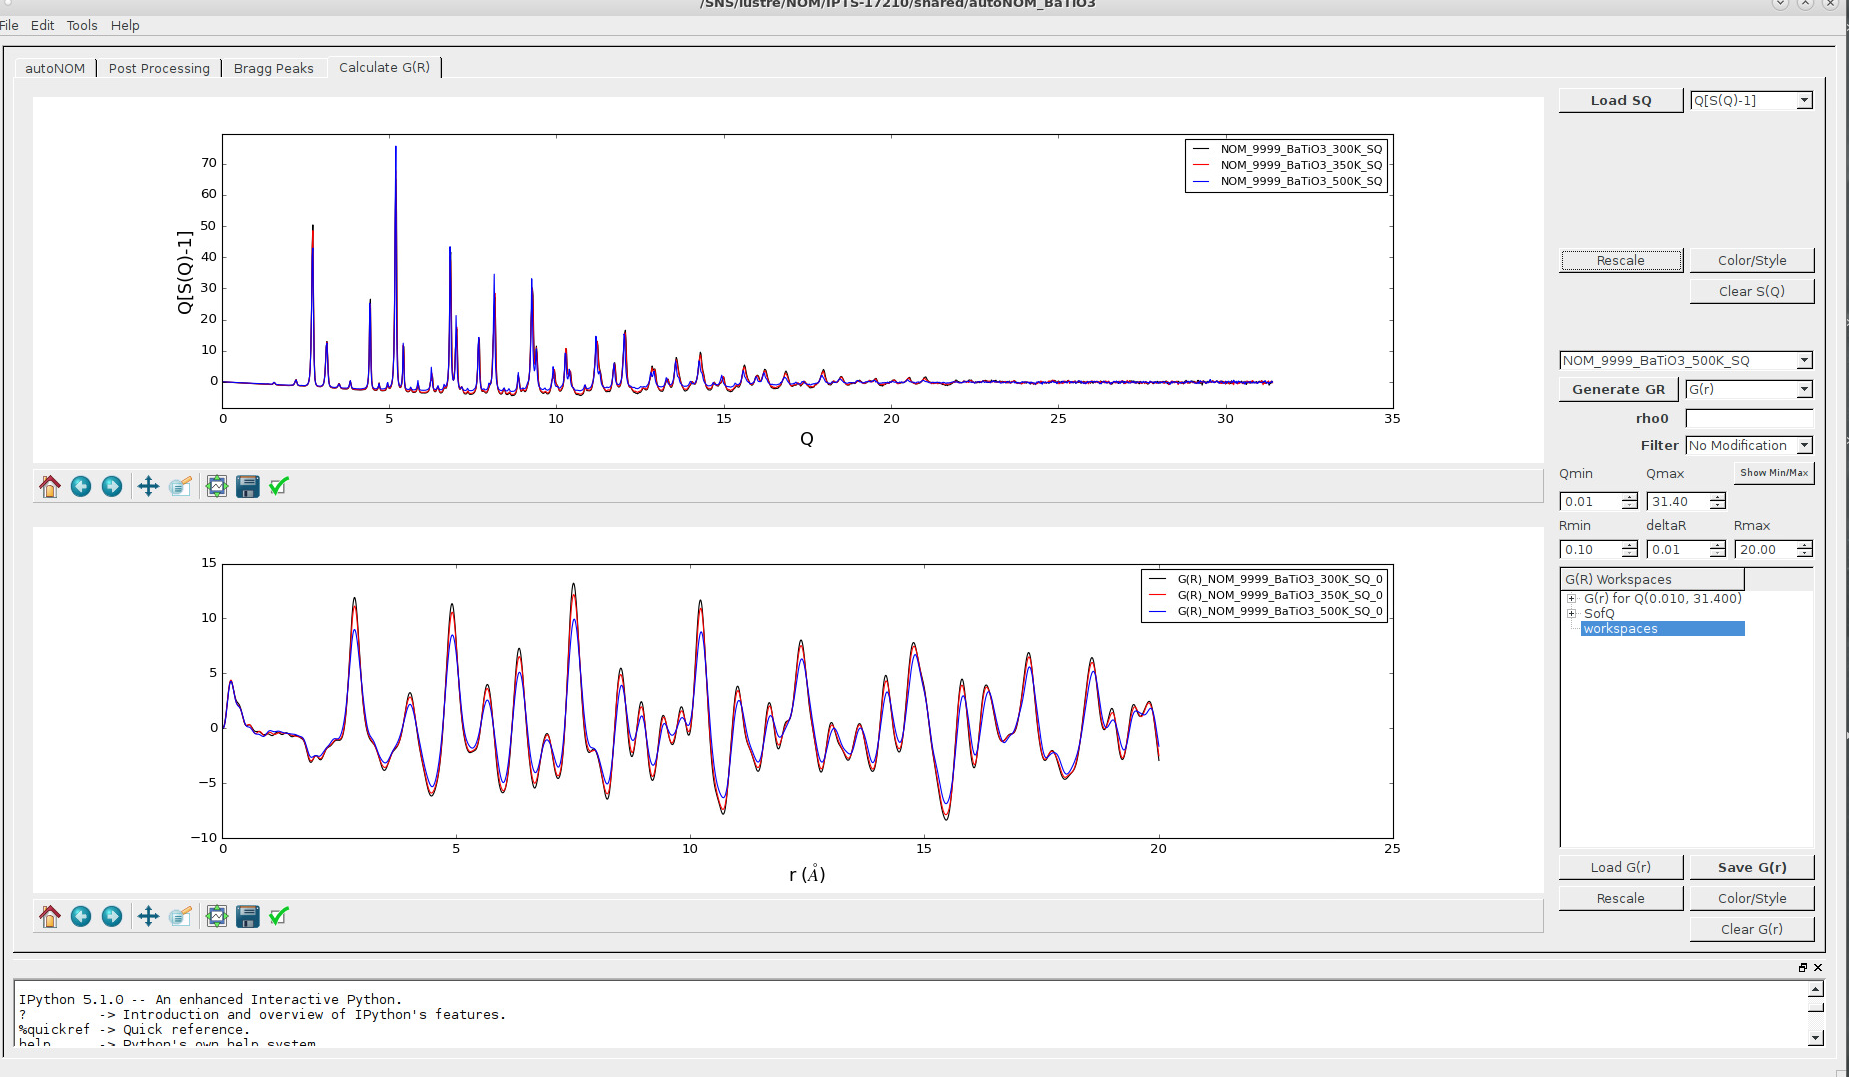
\includegraphics[width=0.9\paperwidth]{graphics/tab4/tab4_populatedGraph_QSofQminus1.png}}

Below this, we have the \guicmd{Rescale} button. If we change the previous drop-down back to \guicmd{S(Q)}, we get the following in the display:

\noindent\makebox[\textwidth]{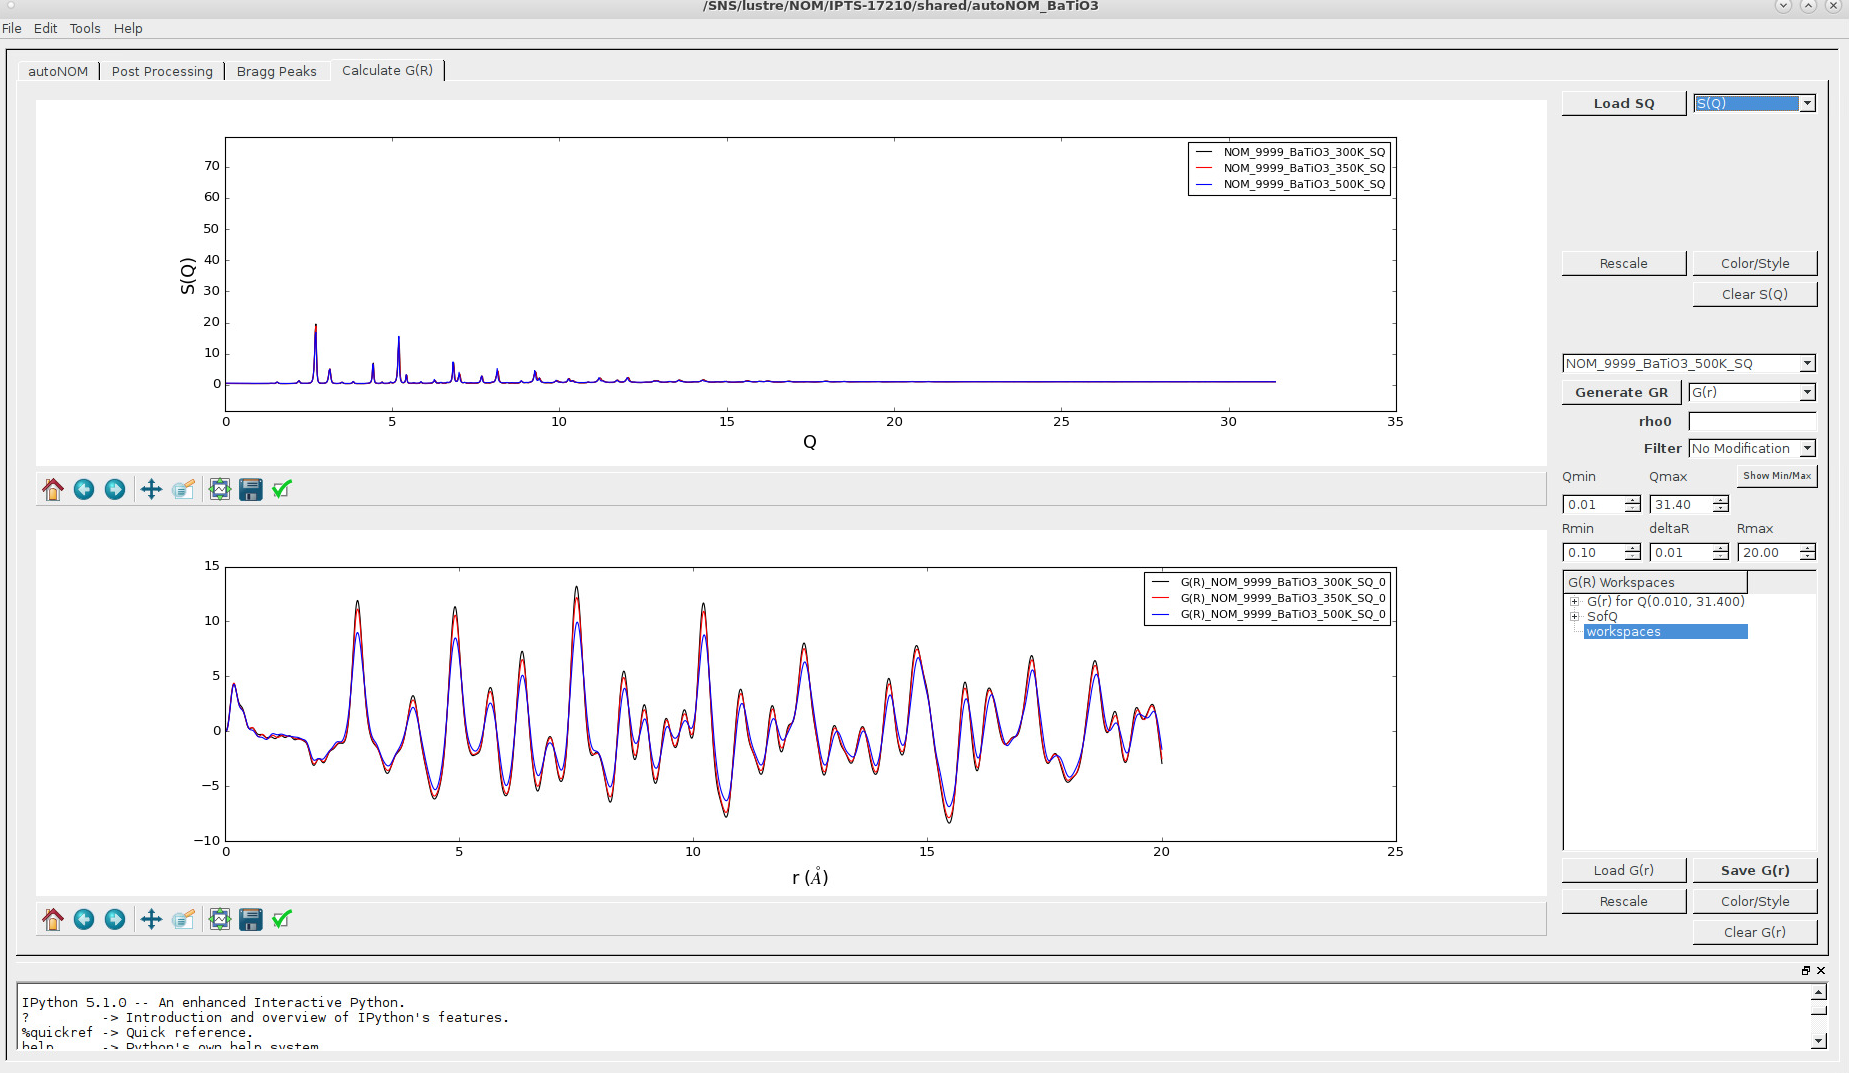
\includegraphics[width=0.9\paperwidth]{graphics/tab4/tab4_populatedGraph_rescaleNeeded.png}}

Clearly, the figure needs to be rescaled to display the data properly. Clicking the \guicmd{Rescale} button, we get back to the previous state for the S(Q) data, as shown below:

\noindent\makebox[\textwidth]{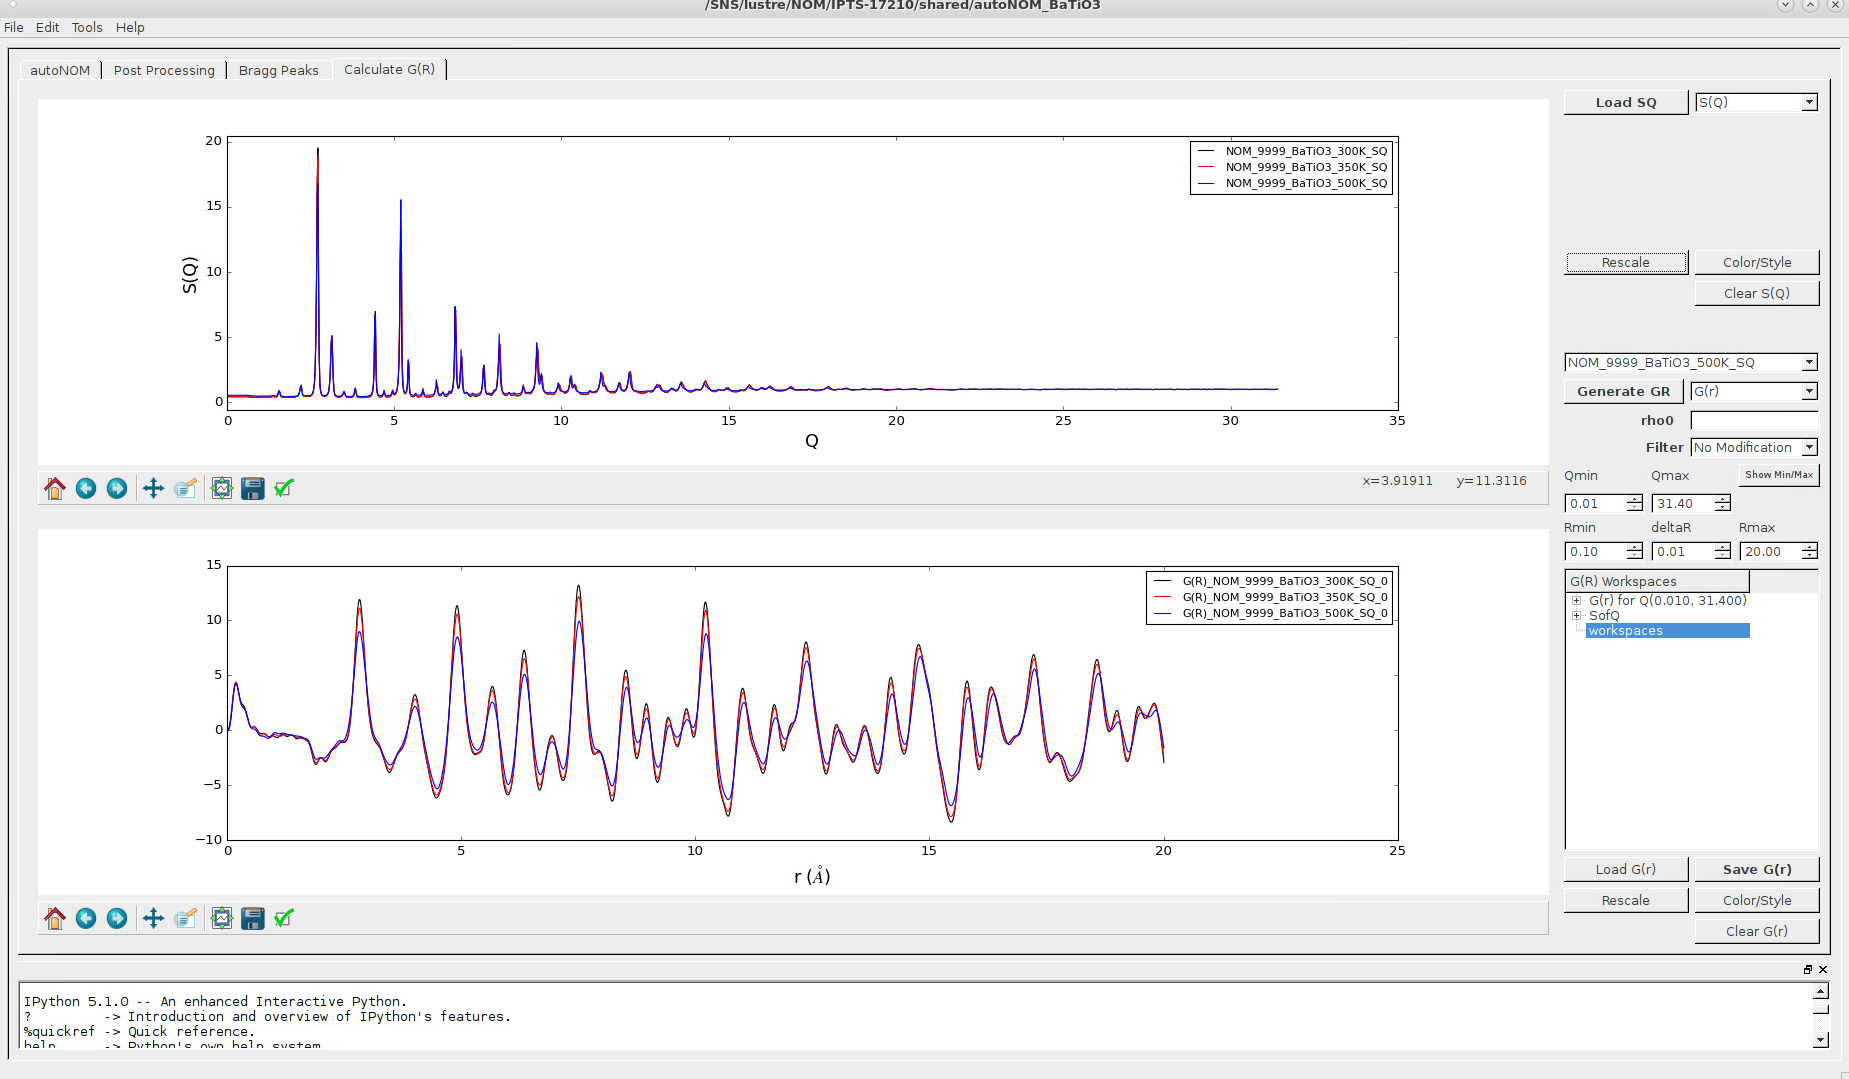
\includegraphics[width=0.9\paperwidth]{graphics/tab4/tab4_populatedGraph_rescaleApplied.png}}

The \guicmd{Color/Style} button can be used to change the display of the S(Q) data in the plot. After pressing the \guicmd{Color/Style} button, we are presented with a file dialog box. We can select the workspace from the drop-down list we would like to change, shown below, and can change the color of the curve, add markers, and select the fill and edge color of the markers from the other drop-downs: 

\noindent\makebox[\textwidth]{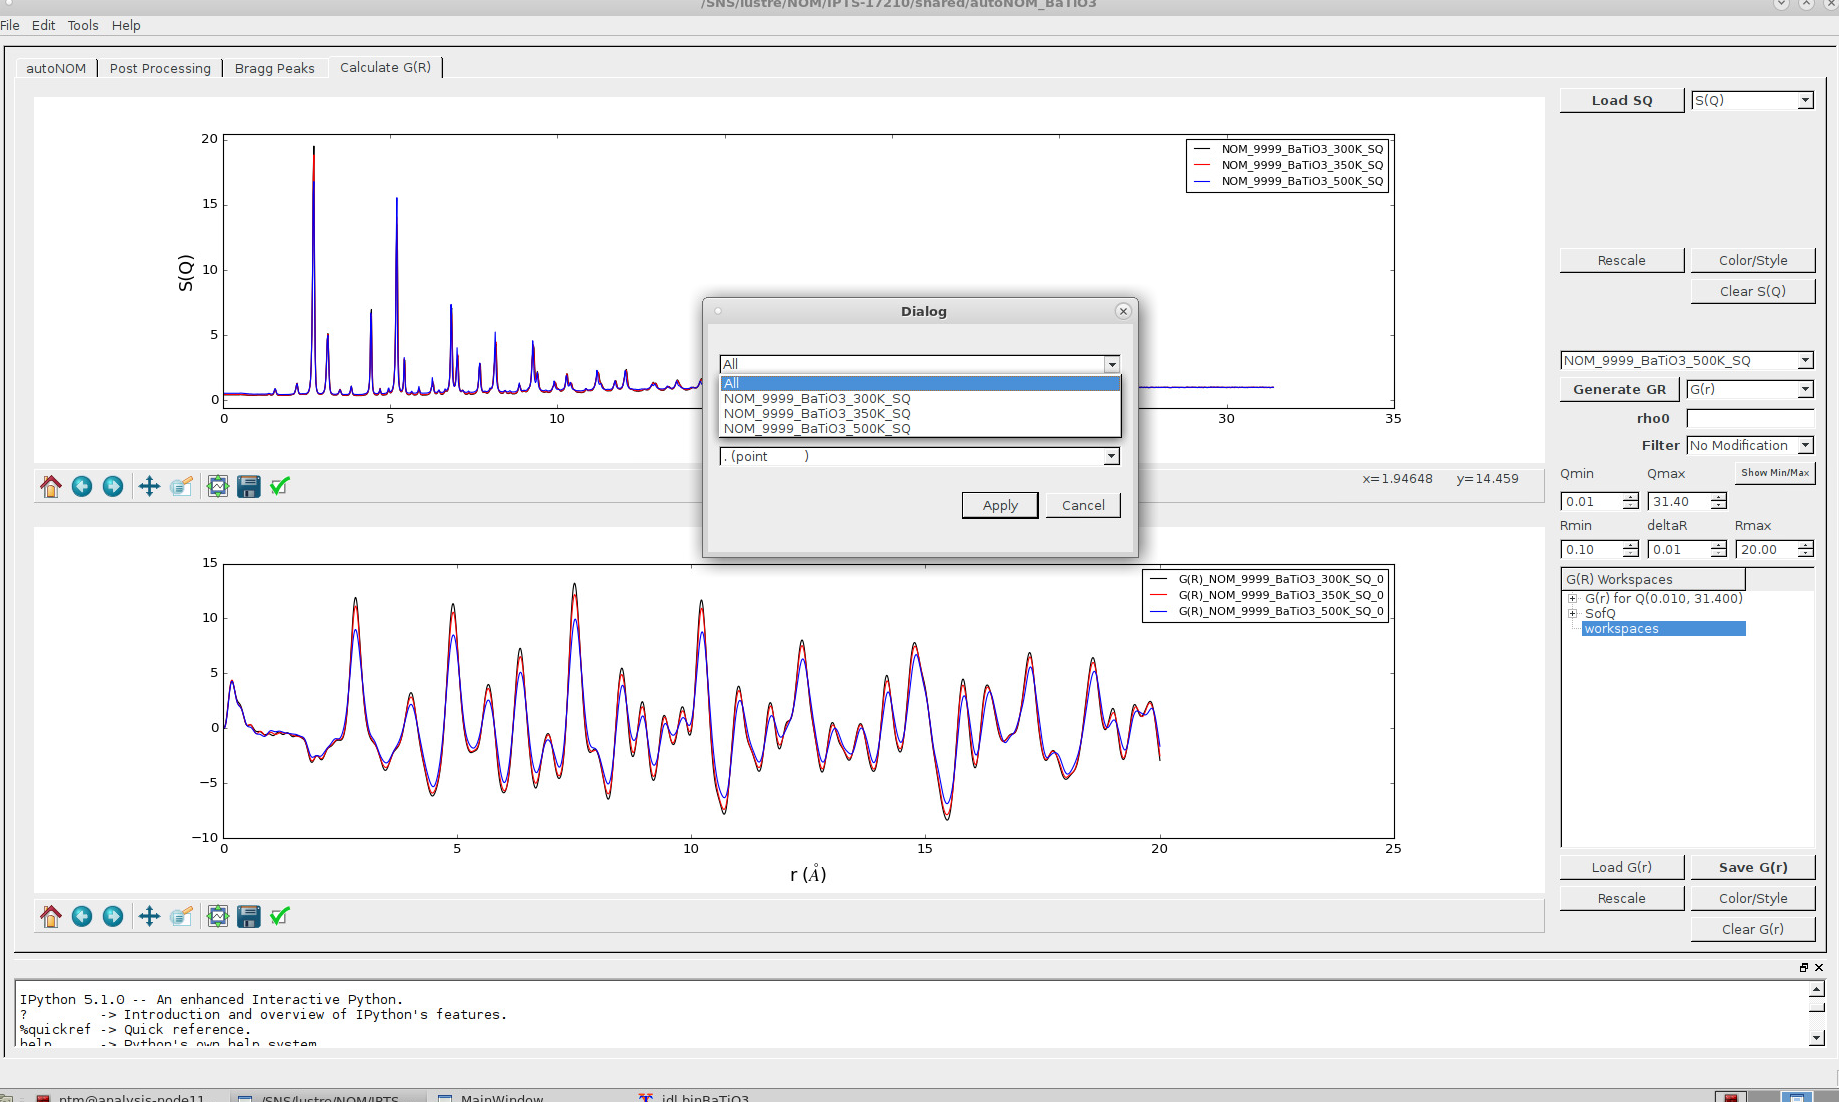
\includegraphics[width=0.9\paperwidth]{graphics/tab4/tab4_populatedGraph_colorStyle.png}}

The \guicmd{CClear S(Q)} button can be used to clear the plotted reciprocal space data sets from the plot view. The datasets are still available to replot in the \guicmd{Workspace Tree}. If we press this from the previous state, we end up with the following below:

\noindent\makebox[\textwidth]{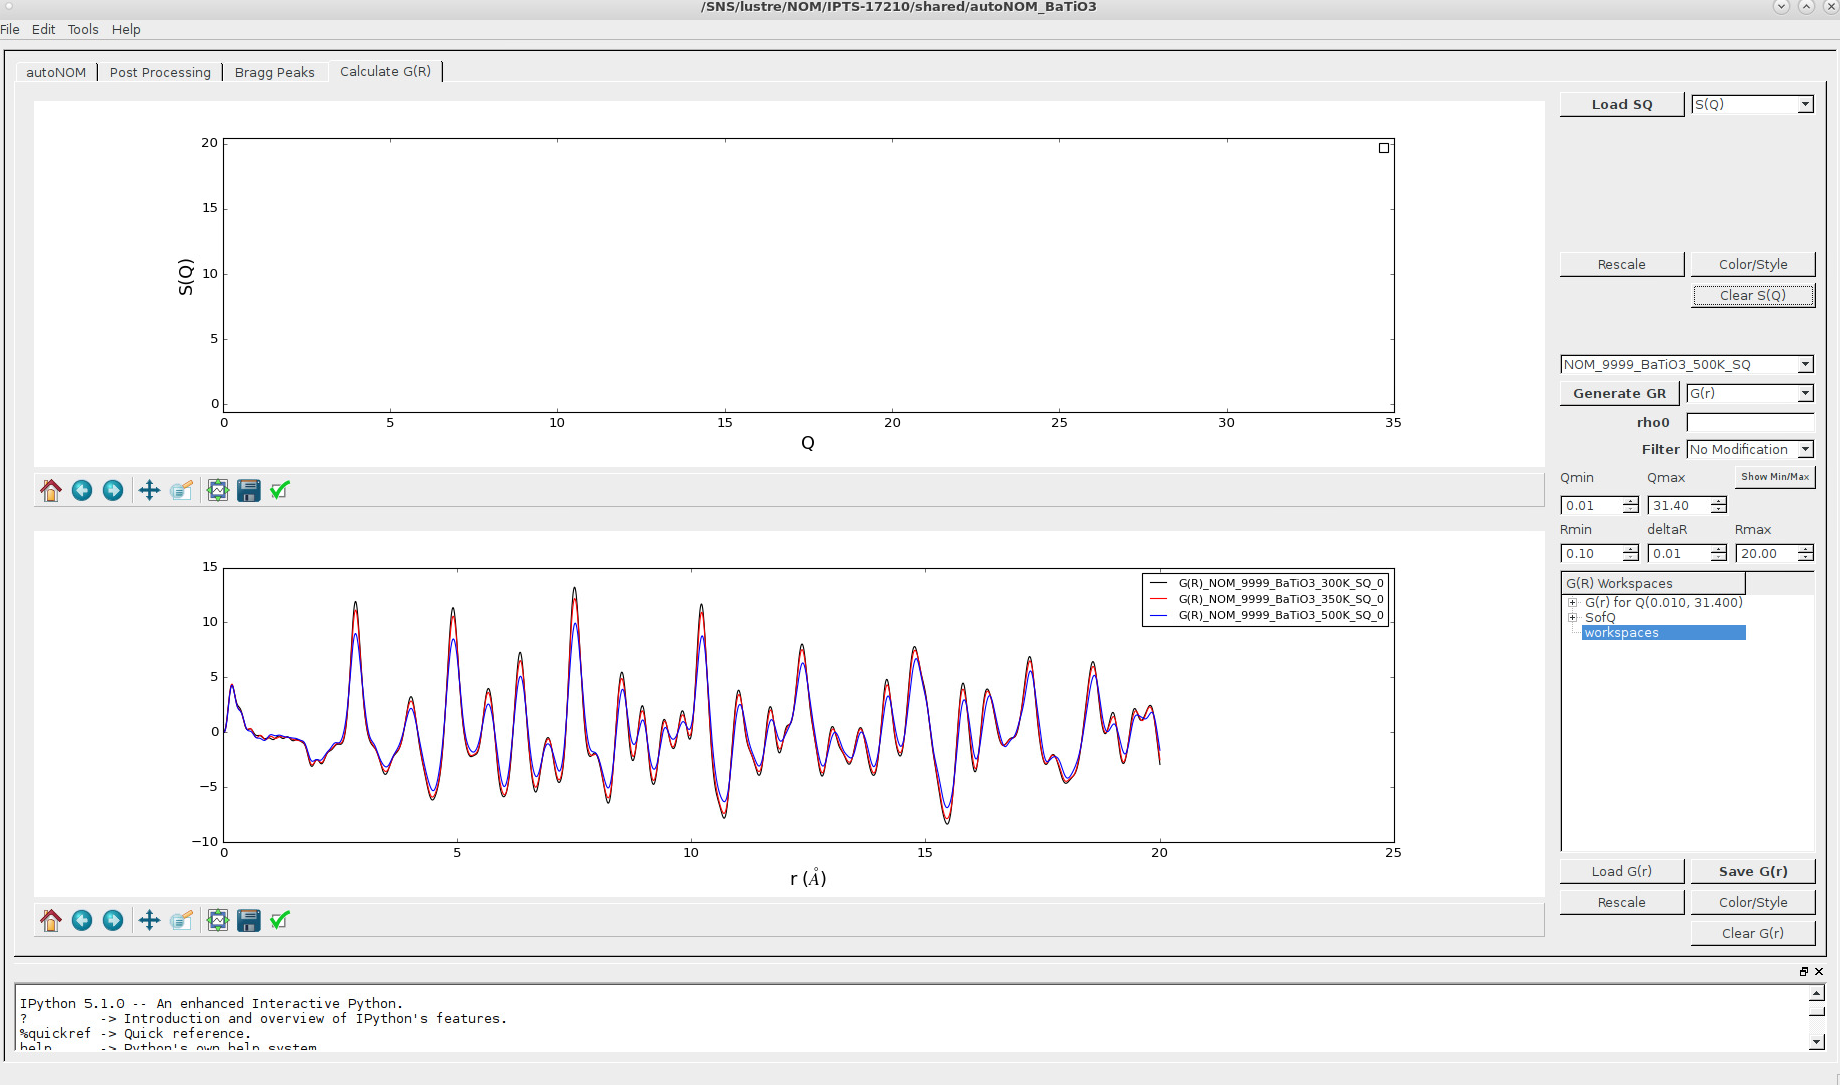
\includegraphics[width=0.9\paperwidth]{graphics/tab4/tab4_populatedGraph_clearSofQ.png}}

In the \guicmd{Workspace Tree}, we can expand the SofQ parent node and see the datasets still available. In the following, we see the datasets are still available even though we cleared the plot view previously:

\noindent\makebox[\textwidth]{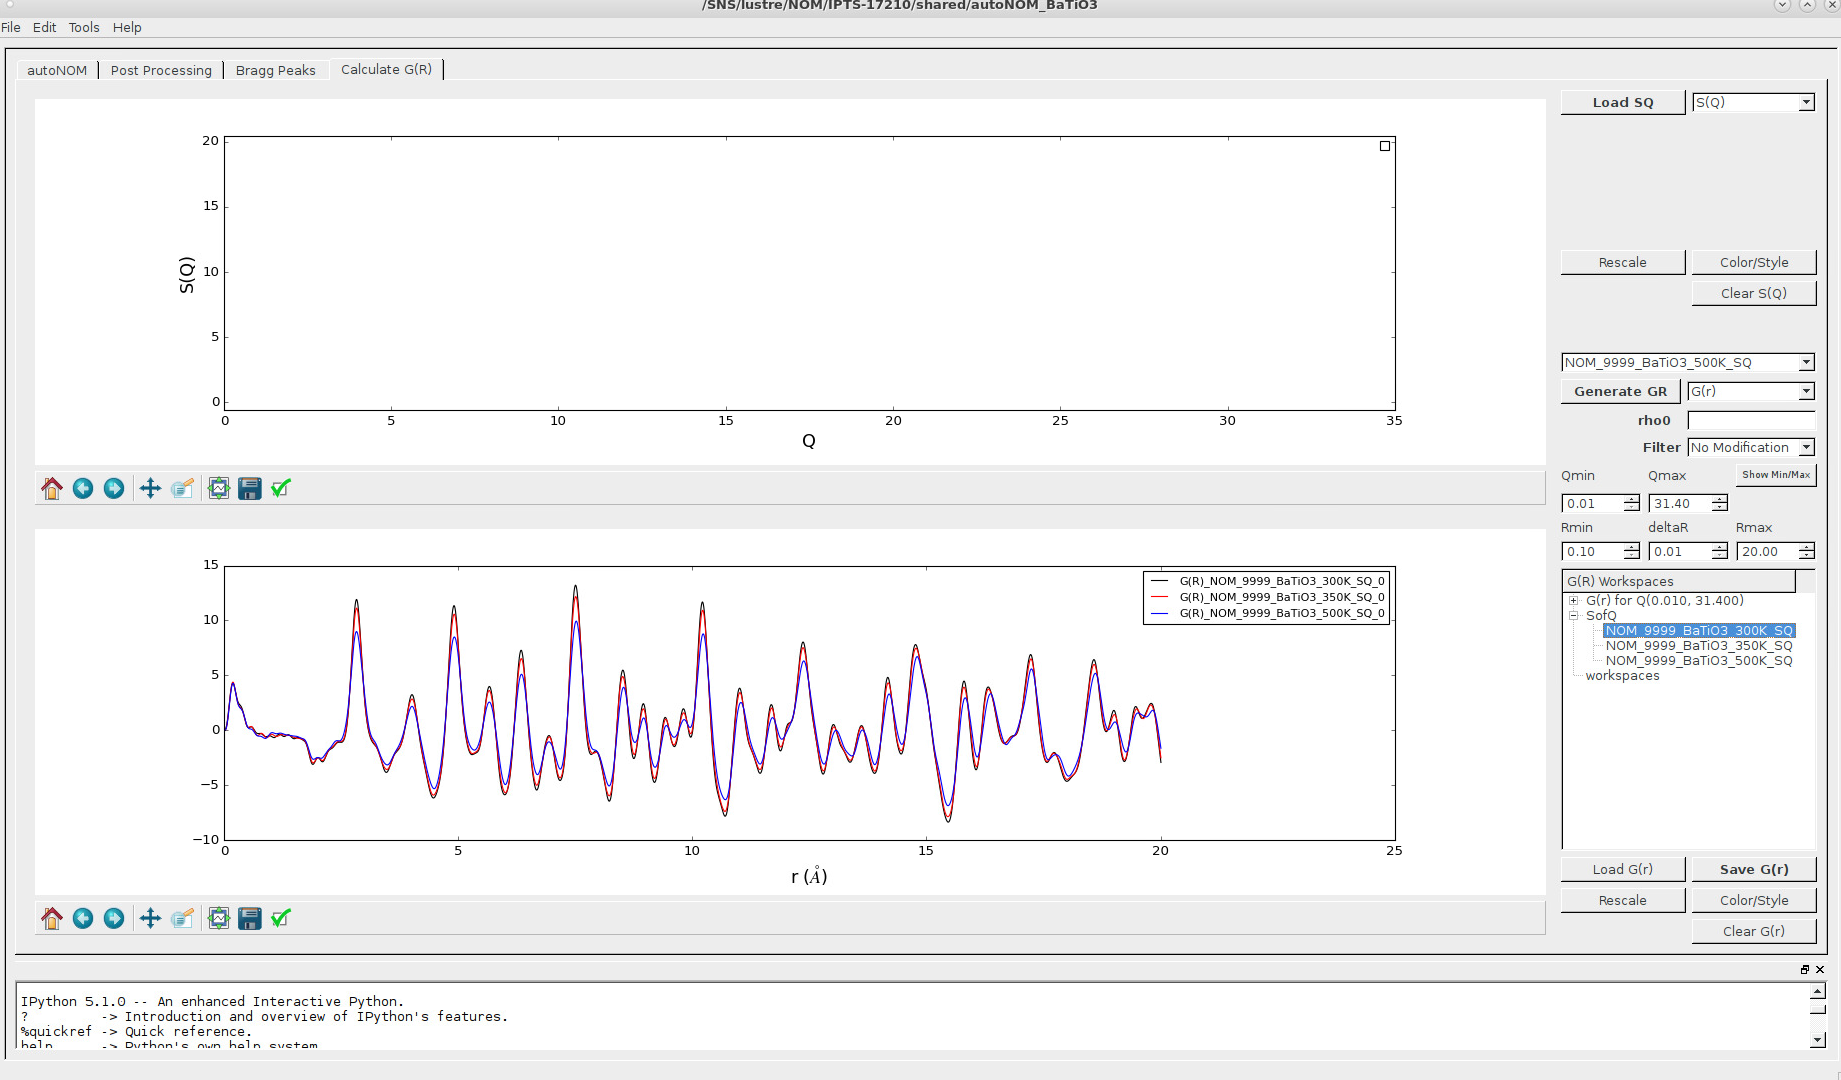
\includegraphics[width=0.9\paperwidth]{graphics/tab4/tab4_populatedGraph_workspaceTree.png}}

Right-clicking any of the data sets in the SofQ workspace tree will give the following options shown below:

\noindent\makebox[\textwidth]{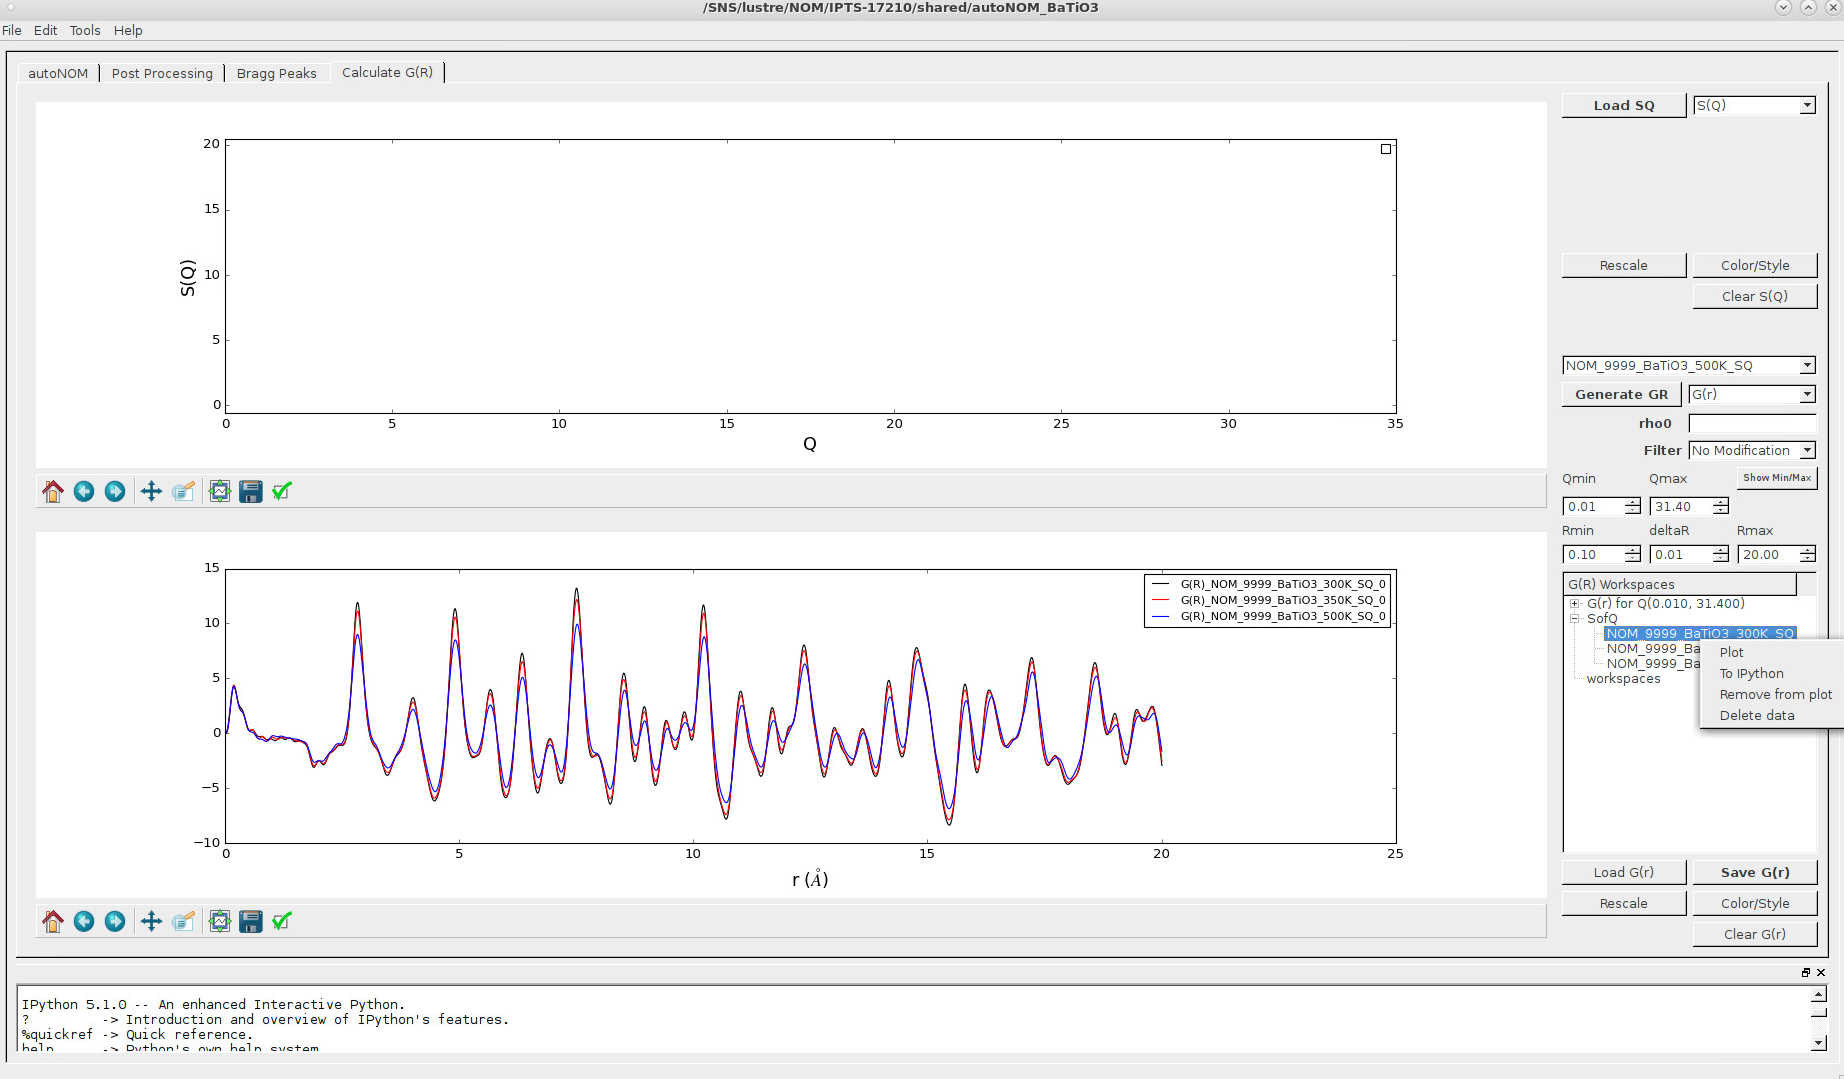
\includegraphics[width=0.9\paperwidth]{graphics/tab4/tab4_populatedGraph_workspaceTree_rightClick.png}}

These options are as follows:
\begin{itemize}

\item \guicmd{Plot}: This will plot the dataset in the S(Q) plot view.
\item \guicmd{To IPython}: Transfer the workspace to the IPython command line dock at the bottom. Here, you can script changes to the workspace and output a new workspace. If clicked, you will have something similar to what is shown below. Here, we have already typed in to add a 2.5 shift:

\noindent\makebox[\textwidth]{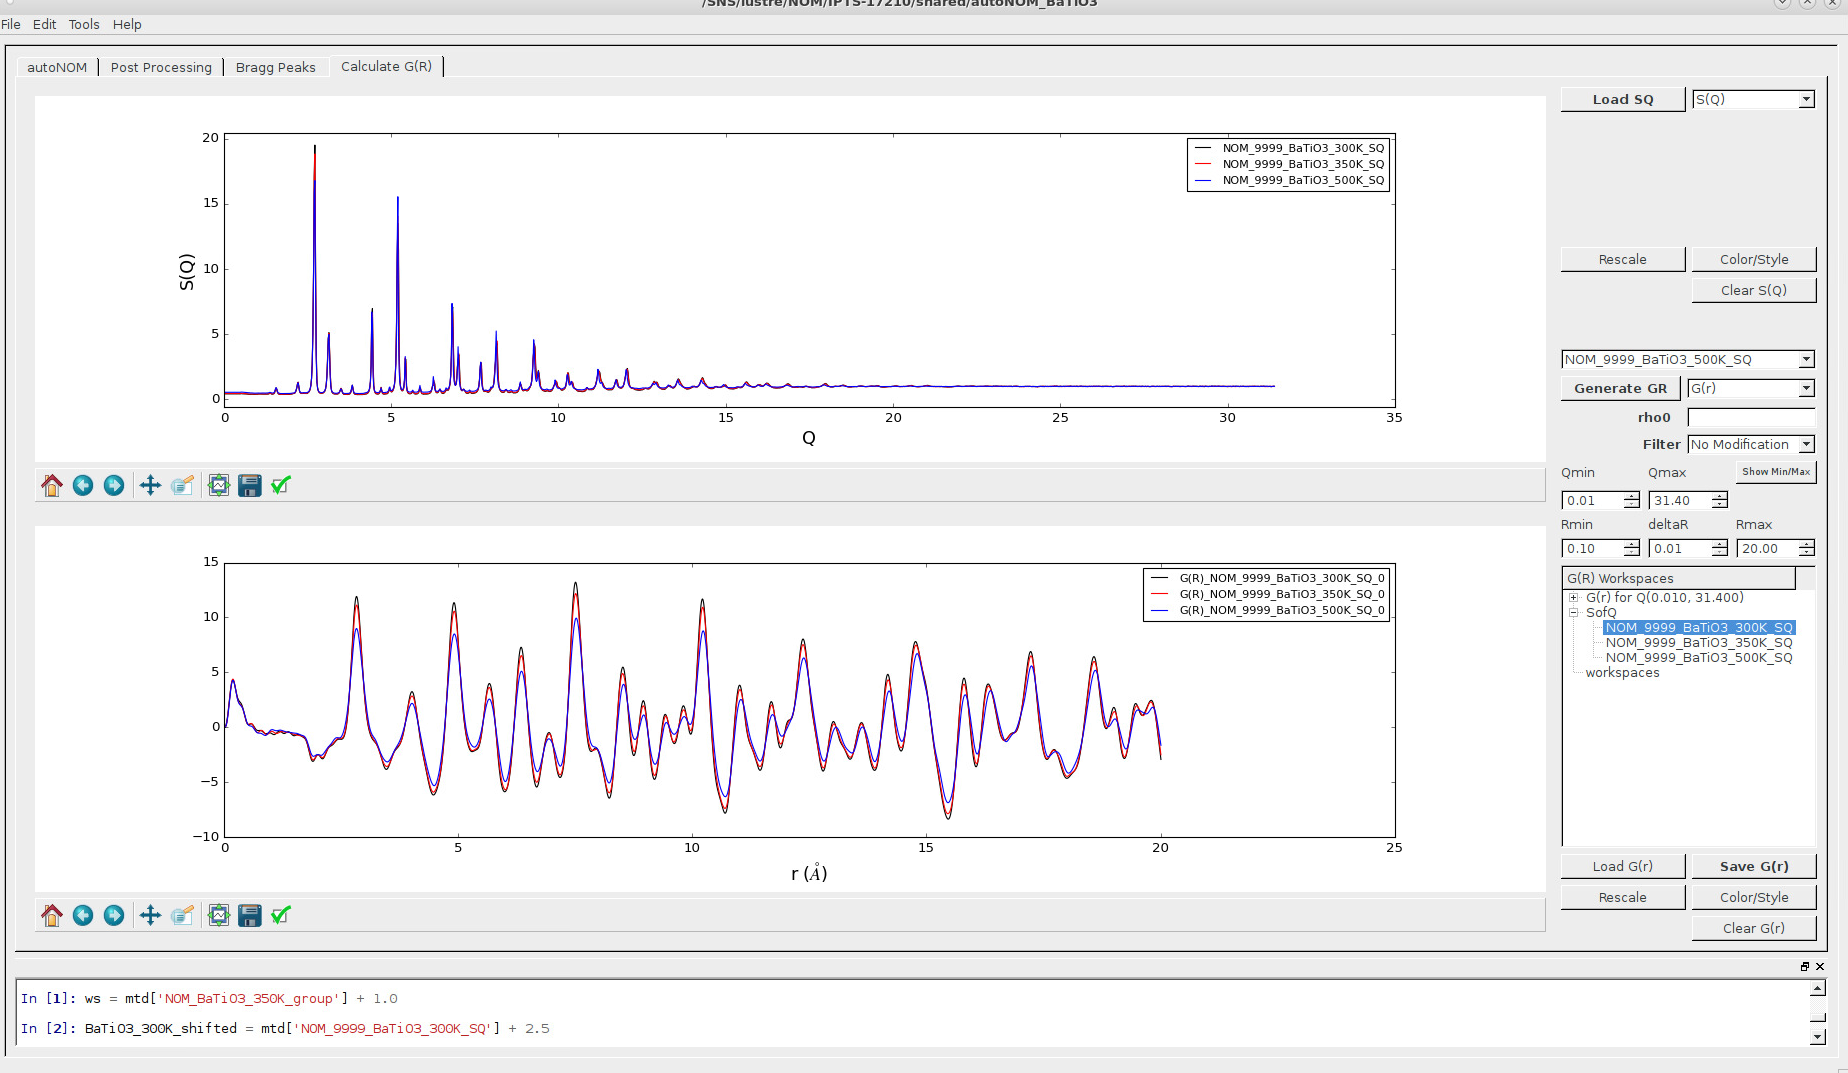
\includegraphics[width=0.9\paperwidth]{graphics/tab4/tab4_populatedGraph_workspaceTree_rightClick_ToIPython.png}}

If we name this new workspace "BaTiO3\_300K\_shifted" and execute the command in the IPython prompt, we will get a new SofQ workspace with this title in the \guicmd{Workspace Tree}. We show below the highlighted workspace in the tree and also have added the plot to the S(Q) plot area: 

\noindent\makebox[\textwidth]{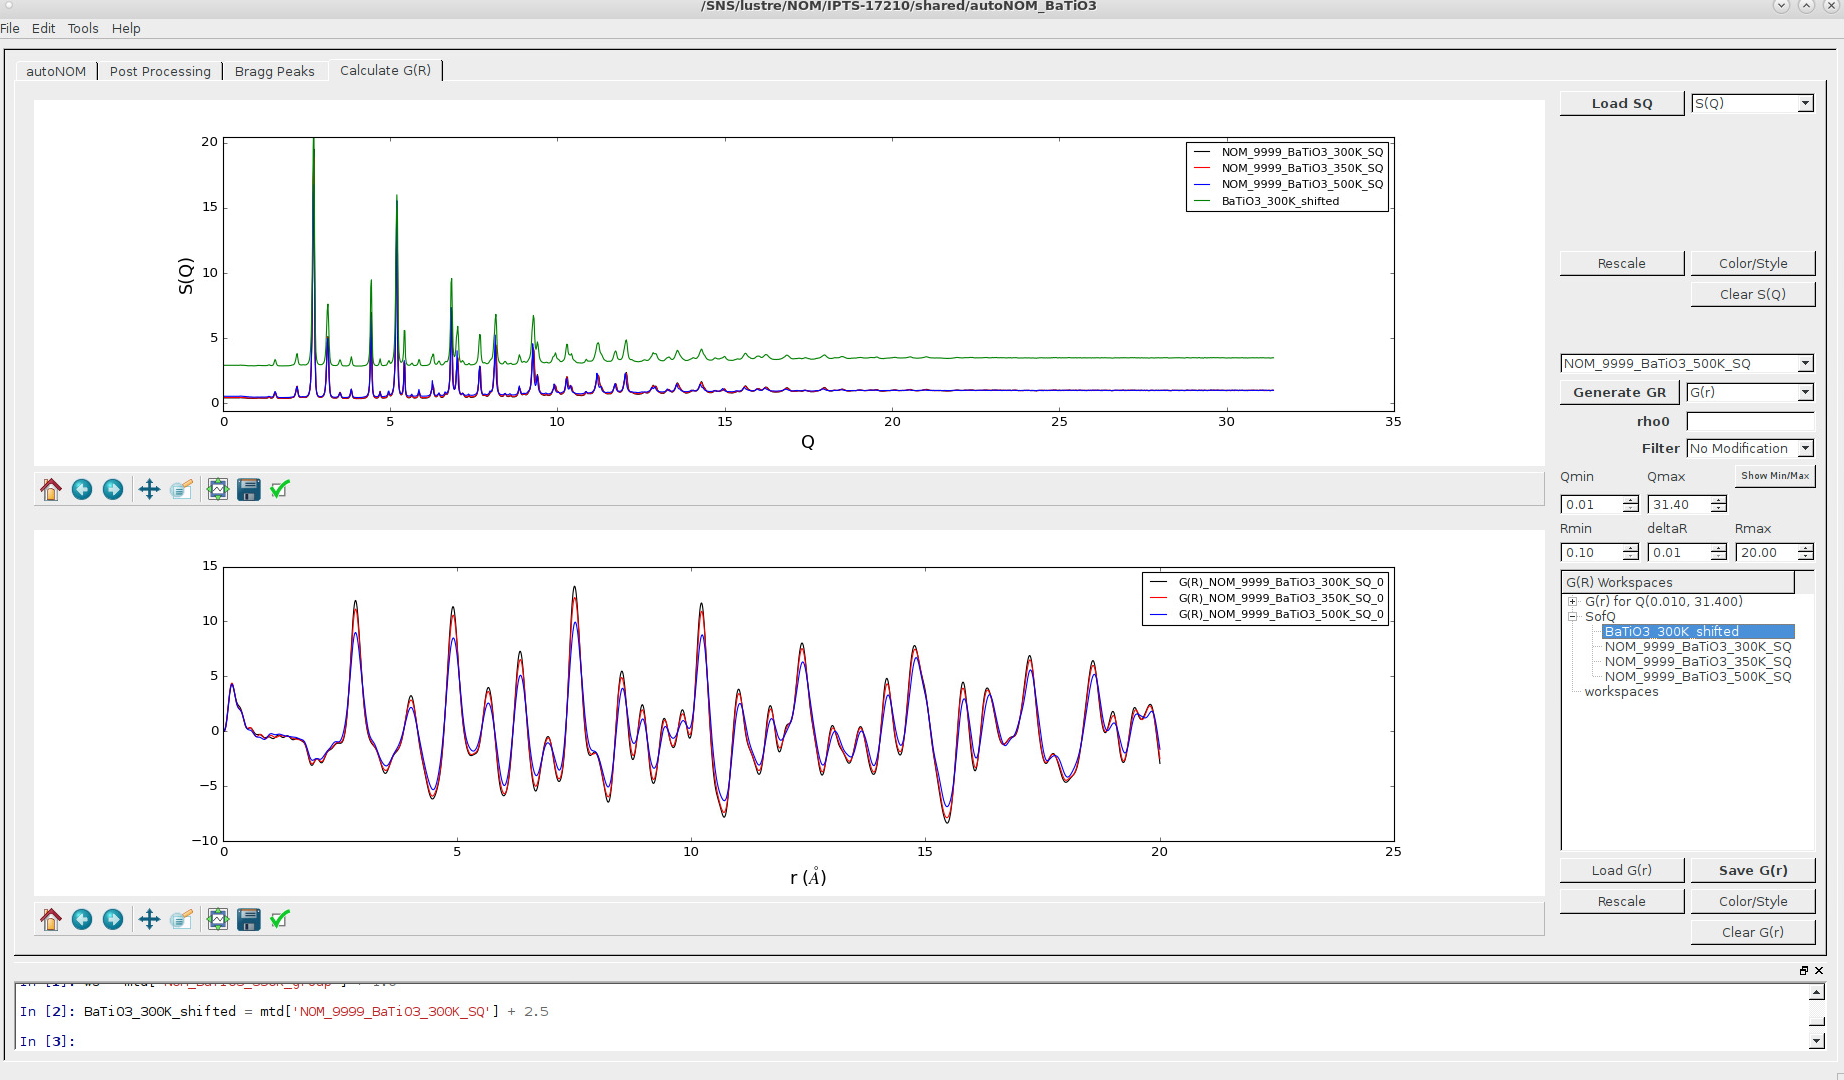
\includegraphics[width=0.9\paperwidth]{graphics/tab4/tab4_populatedGraph_workspaceTree_rightClick_ToIPython_addedToTree.png}}

You can dock and undock the IPython command line prompt by selecting the double-window icon on the top right of the dock, explained previously in the \guicmd{Bragg Peak} tab section.

\item \guicmd{Remove from plotting}: Removes dataset from the plot.
\item \guicmd{Delete data}: Deletes the dataset from the \guicmd{Workspace Tree}.

\end{itemize}

From the drop-down box above the \guicmd{Generate G(r)} button, we can select the new S(Q) workspace. Then, we can press the \guicmd{Generate G(r)} button to perform the Fourier transform on this S(Q) dataset. We see that the new G(r) dataset shows up as a workspace in the \guicmd{Workspace Tree} under the G(r) subtree. We show an example of this below:

\noindent\makebox[\textwidth]{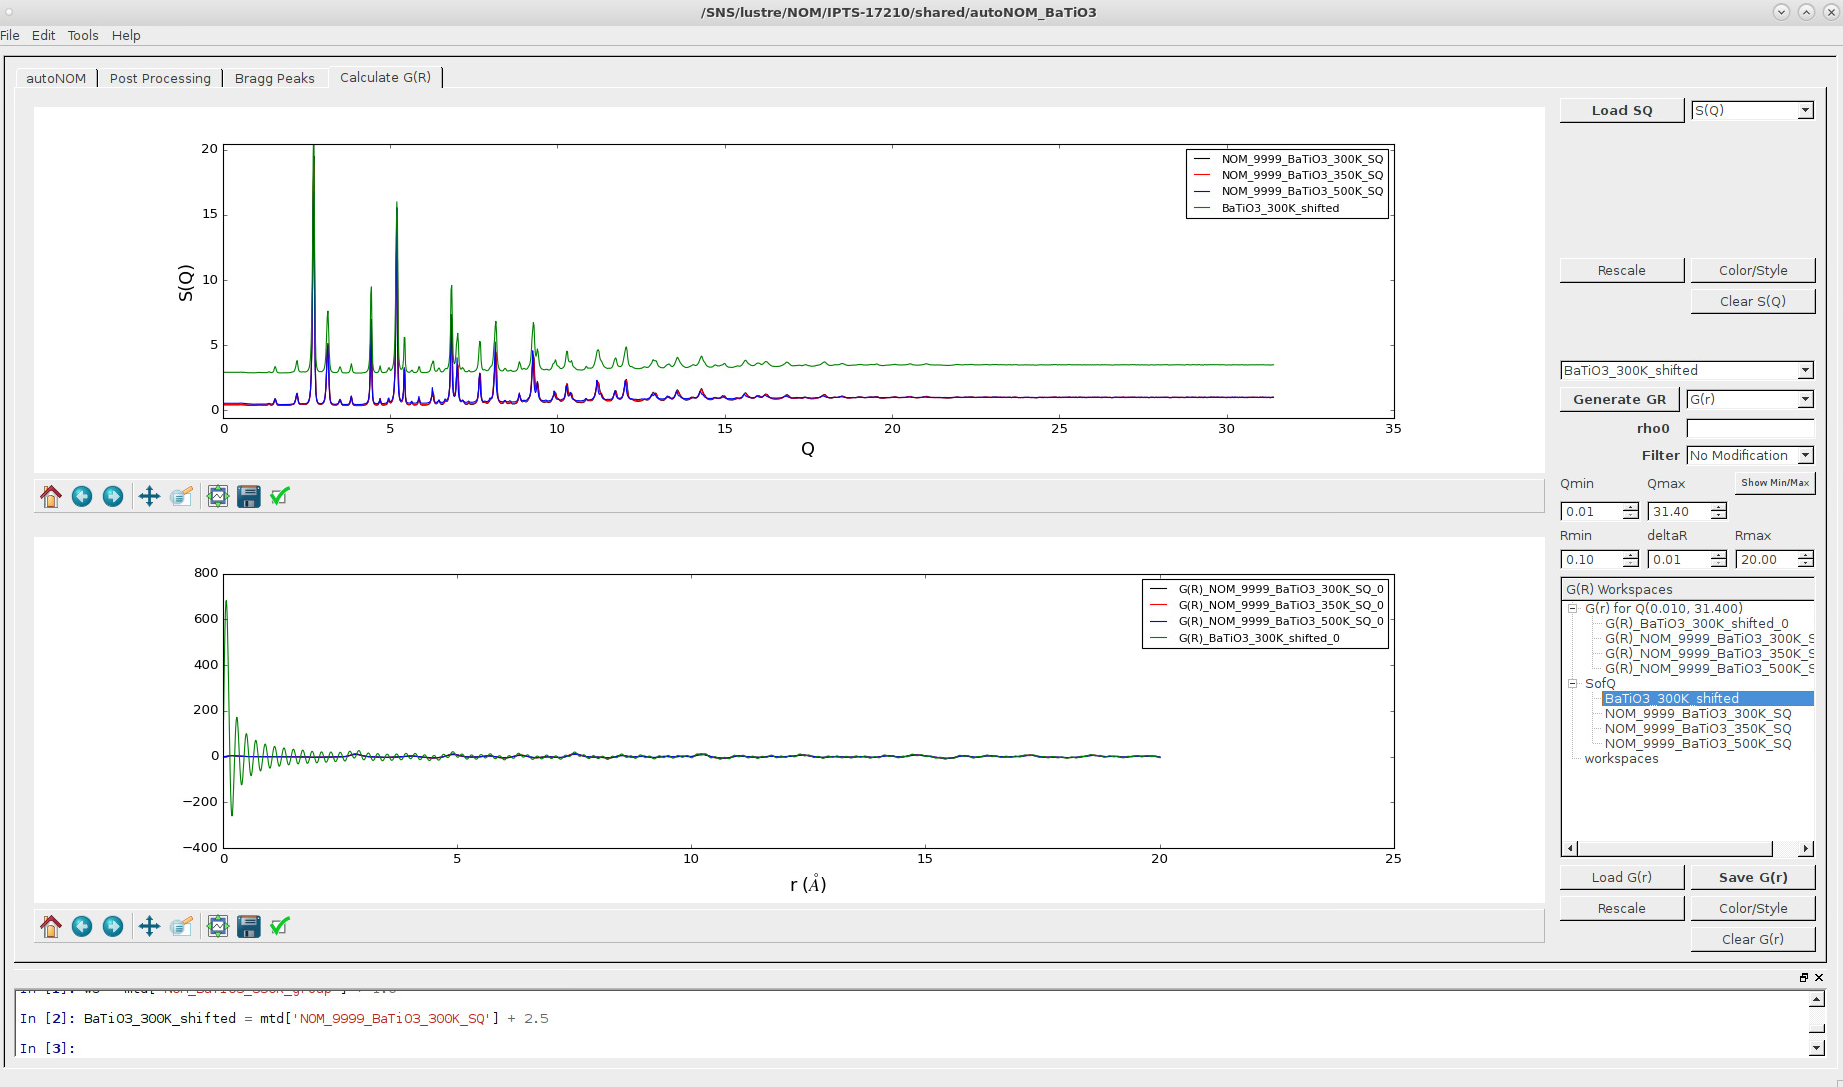
\includegraphics[width=0.9\paperwidth]{graphics/tab4/tab4_populatedGraph_workspaceTree_GofR.png}}

Also, from the drop-down beside the \guicmd{Generate G(r)} button, we can also select to generate \guicmd{g(r)} or \guicmd{RDF} (the Radial Distrbution Function).

If we right-click, we see that we have the same options for the G(r) workspaces as for the S(Q) workspaces:

\noindent\makebox[\textwidth]{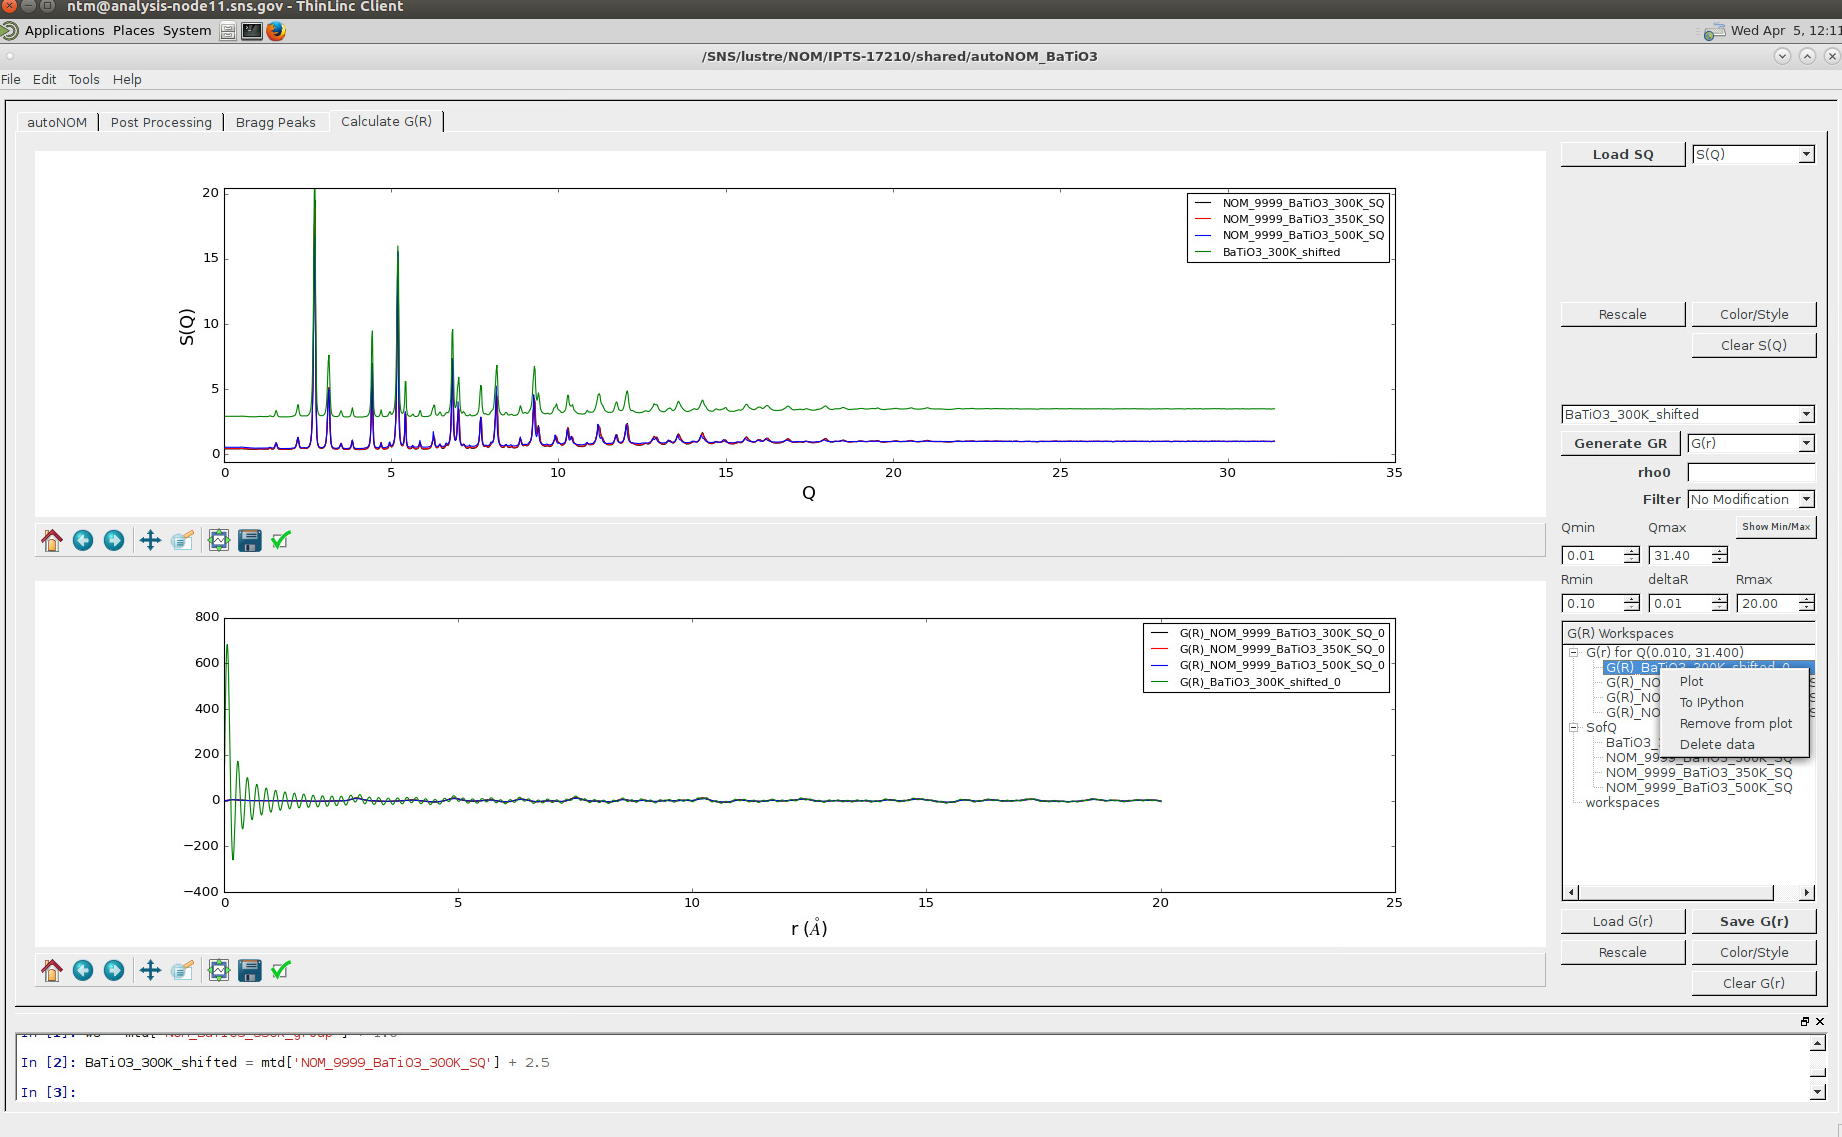
\includegraphics[width=0.9\paperwidth]{graphics/tab4/tab4_populatedGraph_workspaceTree_GofR_rightClick.png}}

Below, we have removed the G(r) workspace that was just created from the plot(the \guicmd{G(r) BaTiO3\_300K\_shifted\_0} workspace). Notice, it still exists in the \guicmd{Workspace Tree}:

\noindent\makebox[\textwidth]{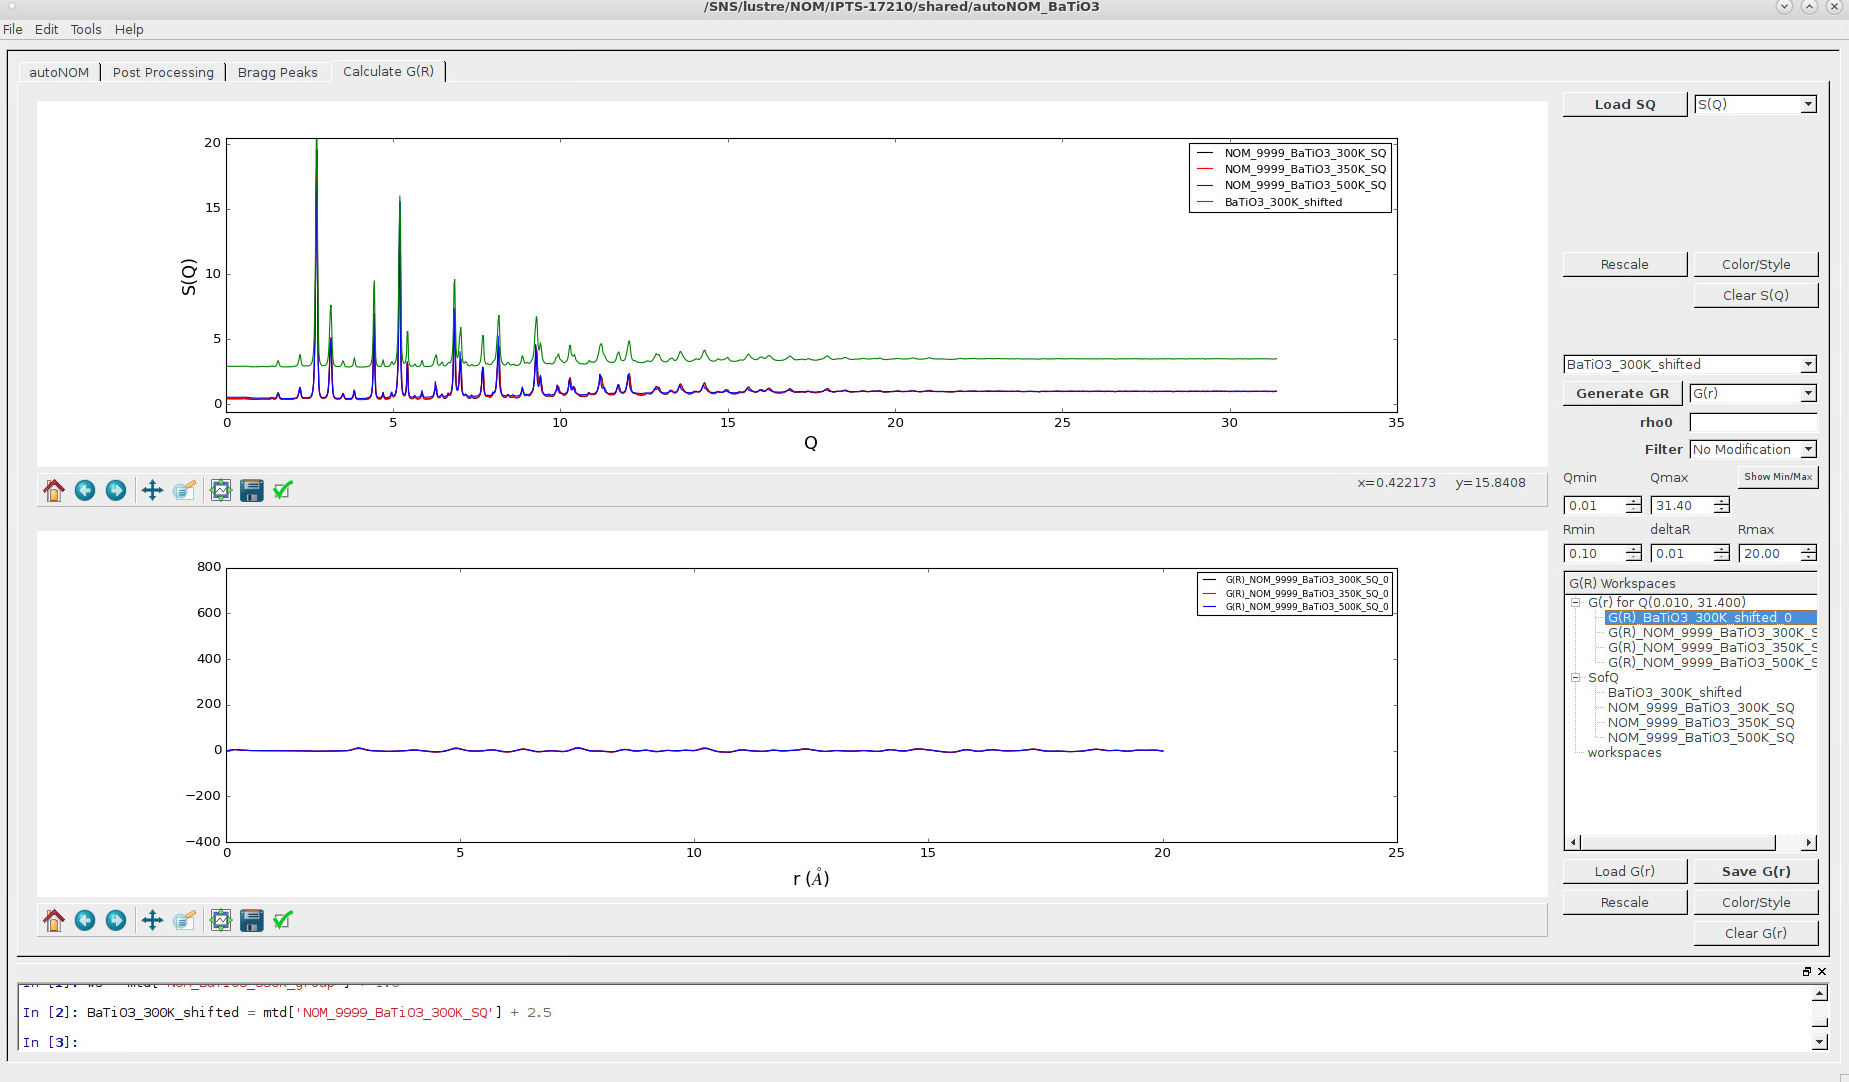
\includegraphics[width=0.9\paperwidth]{graphics/tab4/tab4_populatedGraph_workspaceTree_GofR_rightClick_removeFromPlot.png}}

Now, we can also delete the G(r) workspace.. Notice, it no longer exists in the \guicmd{Workspace Tree}:

\noindent\makebox[\textwidth]{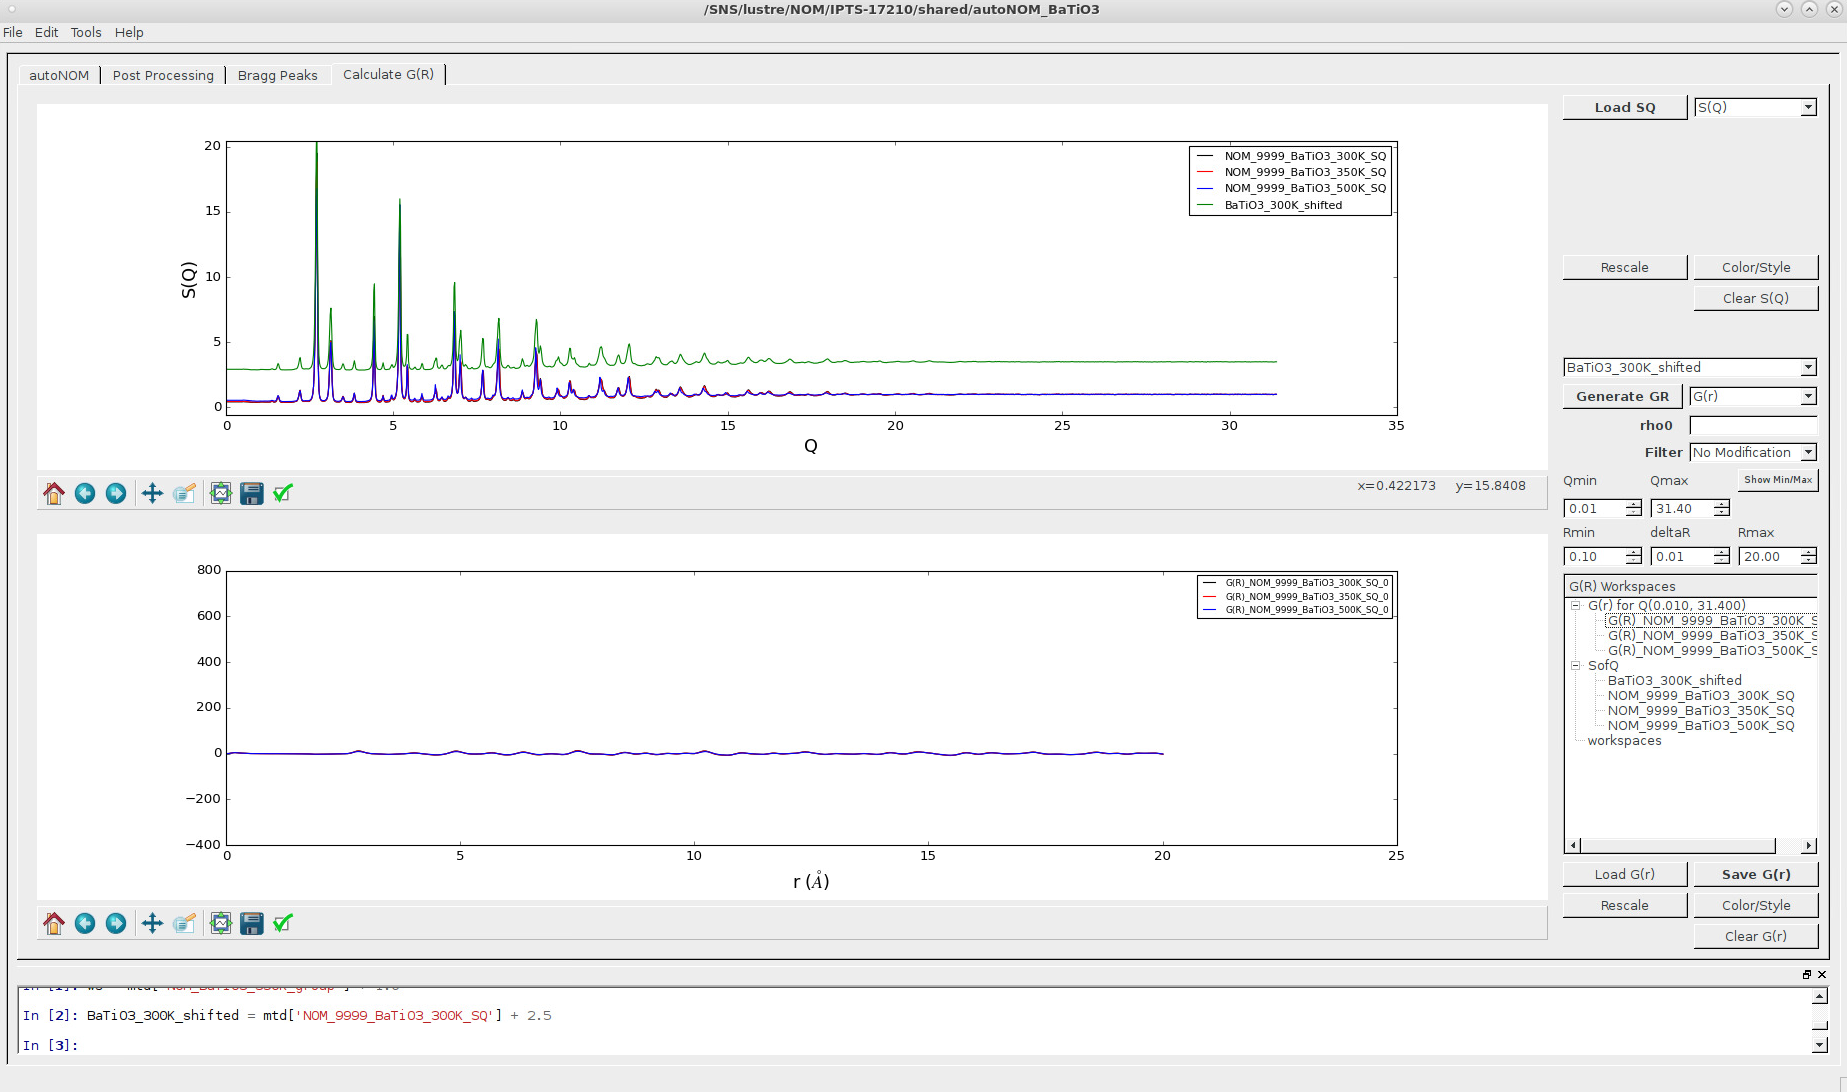
\includegraphics[width=0.9\paperwidth]{graphics/tab4/tab4_populatedGraph_workspaceTree_GofR_rightClick_deleteData.png}}

The \guicmd{rho0} field is used to input a bulk density value.

The \guicmd{Filter} drop-down is used to select different function we can use to transform and modify our data. Currently, the options are to apply no such function,  \guicmd{No Modification}, or to use the \guicmd{Lorch} function. Multiplication with a Lorch function reduced the influence of high Q noise and leads to smoother G(r)/PDF data. However, this comes at the expense of real space resolution (multiplication in Q = convolution in r).

The \guicmd{Qmin} and \guicmd{Qmax} specify over what Q range to perform the Fourier transform to produce a G(r). If we press the \guicmd{Show Min/Max}, we get a visual display in the S(Q) plot area of these \guicmd{Qmin} and \guicmd{Qmax} values we are using. An example is shown below:

\noindent\makebox[\textwidth]{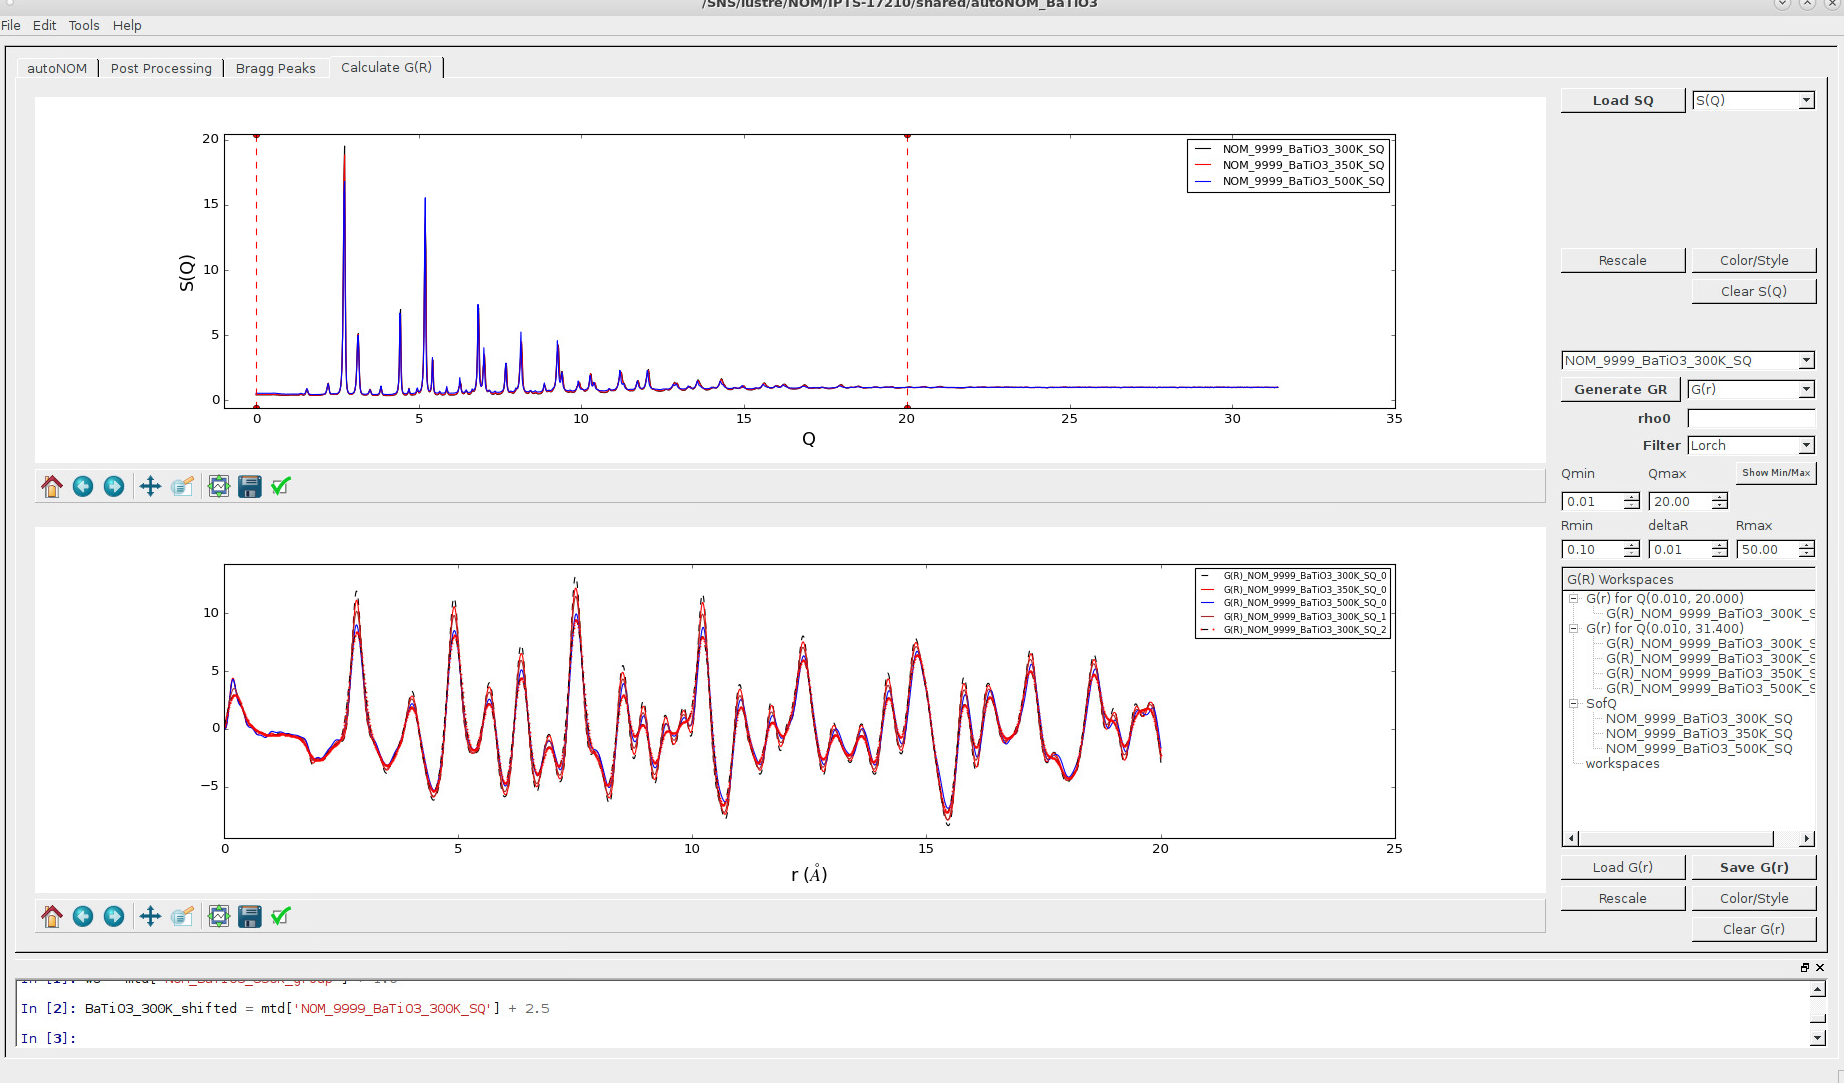
\includegraphics[width=0.9\paperwidth]{graphics/tab4/tab4_populatedGraph_differentQmaxTree.png}}

The \guicmd{Rmin} and \guicmd{Rmax} specify the minimum and maximum value of the real space data, respectively. The \guicmd{deltaR} specifies the bin size used for the produced G(r). Below, we show where we have extended the Rmax range for the G(r) produced:

\noindent\makebox[\textwidth]{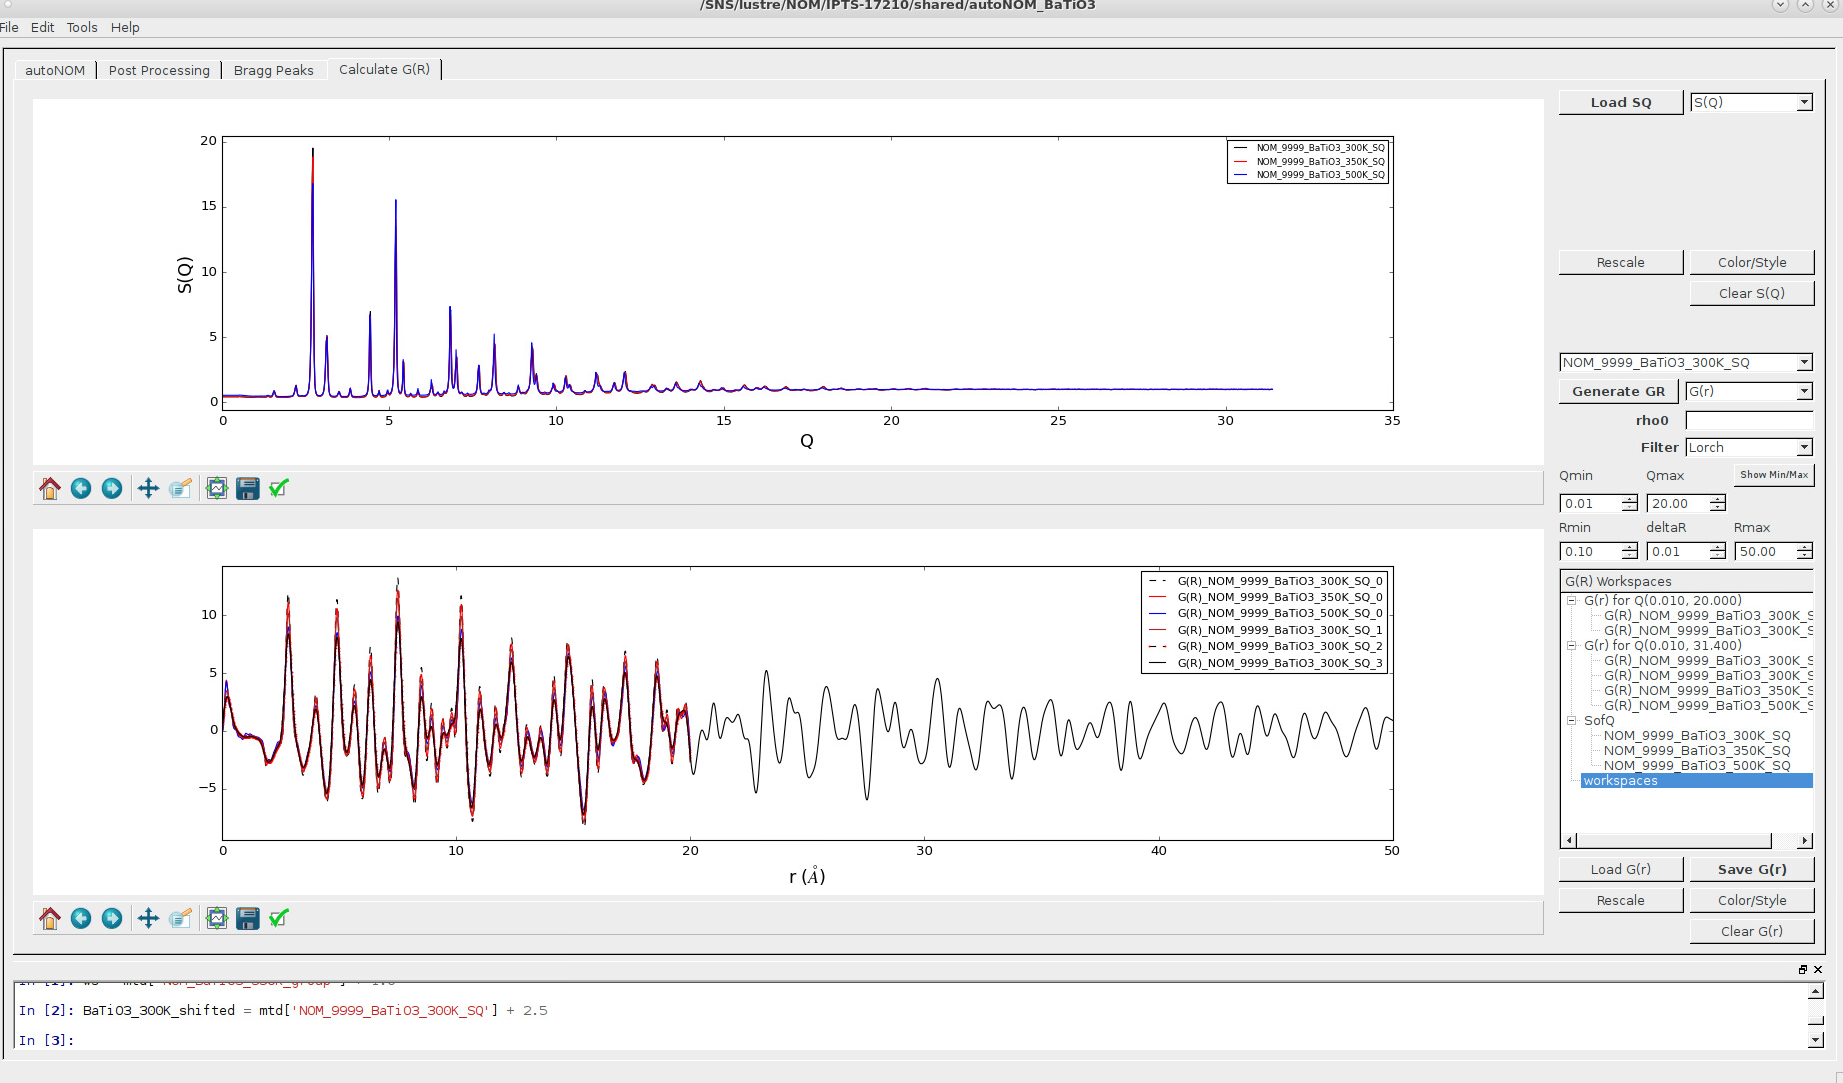
\includegraphics[width=0.9\paperwidth]{graphics/tab4/tab4_populatedGraph_extendedRMax.png}}

To change the legend, in case it is in the way or masking data, you can right-click inside any of the plot areas and either reduce the font of the text, increase the font of the text, or hide the legend all together. An example is shown below:

\noindent\makebox[\textwidth]{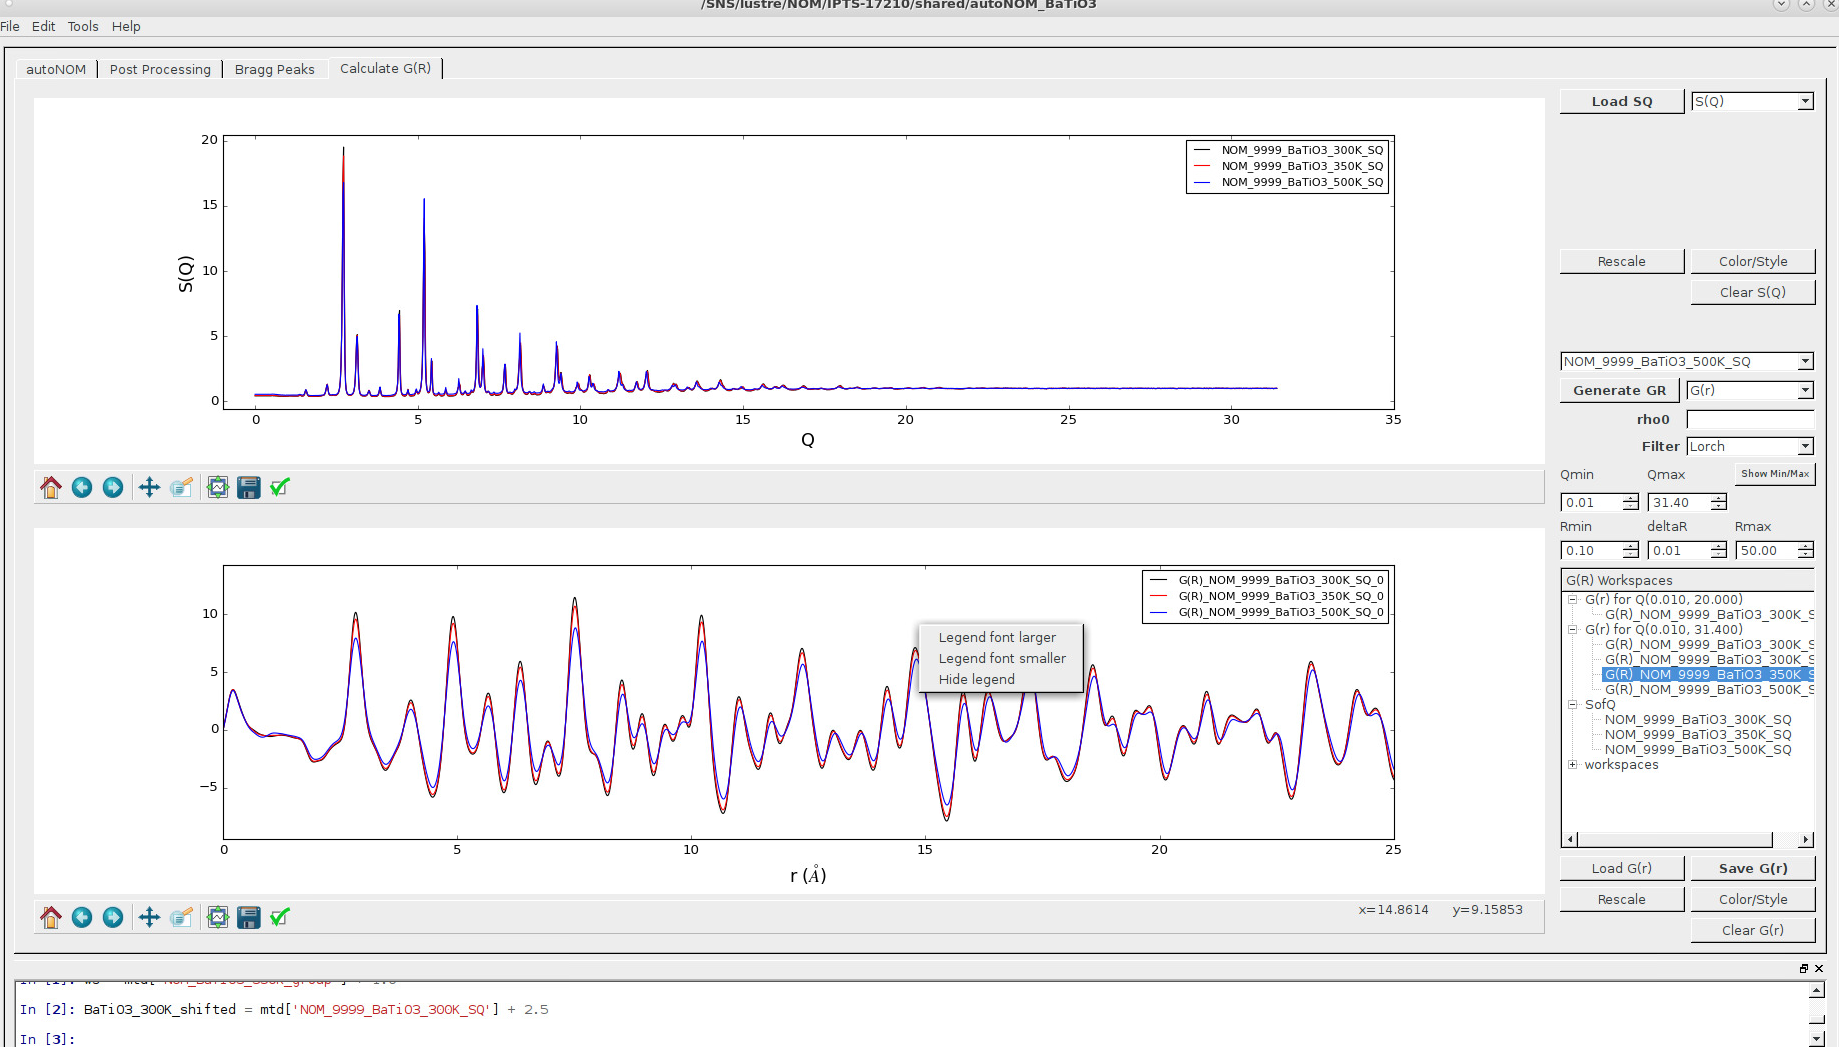
\includegraphics[width=0.9\paperwidth]{graphics/tab4/tab4_populatedGraph_rightClick_legendOptions.png}}

\subsection{Load G(r) data}
We can also load in our real space data from the individual runs or post-processed runs that are complete.  Go to the bottom right and press the \guicmd{Load G(r)} button. You can select either the \fileio{gofr} or the \fileio{PDF} file directories. 

If you choose the \fileio{PDF}, you should be presented with a file dialog similar to the one below:

\noindent\makebox[\textwidth]{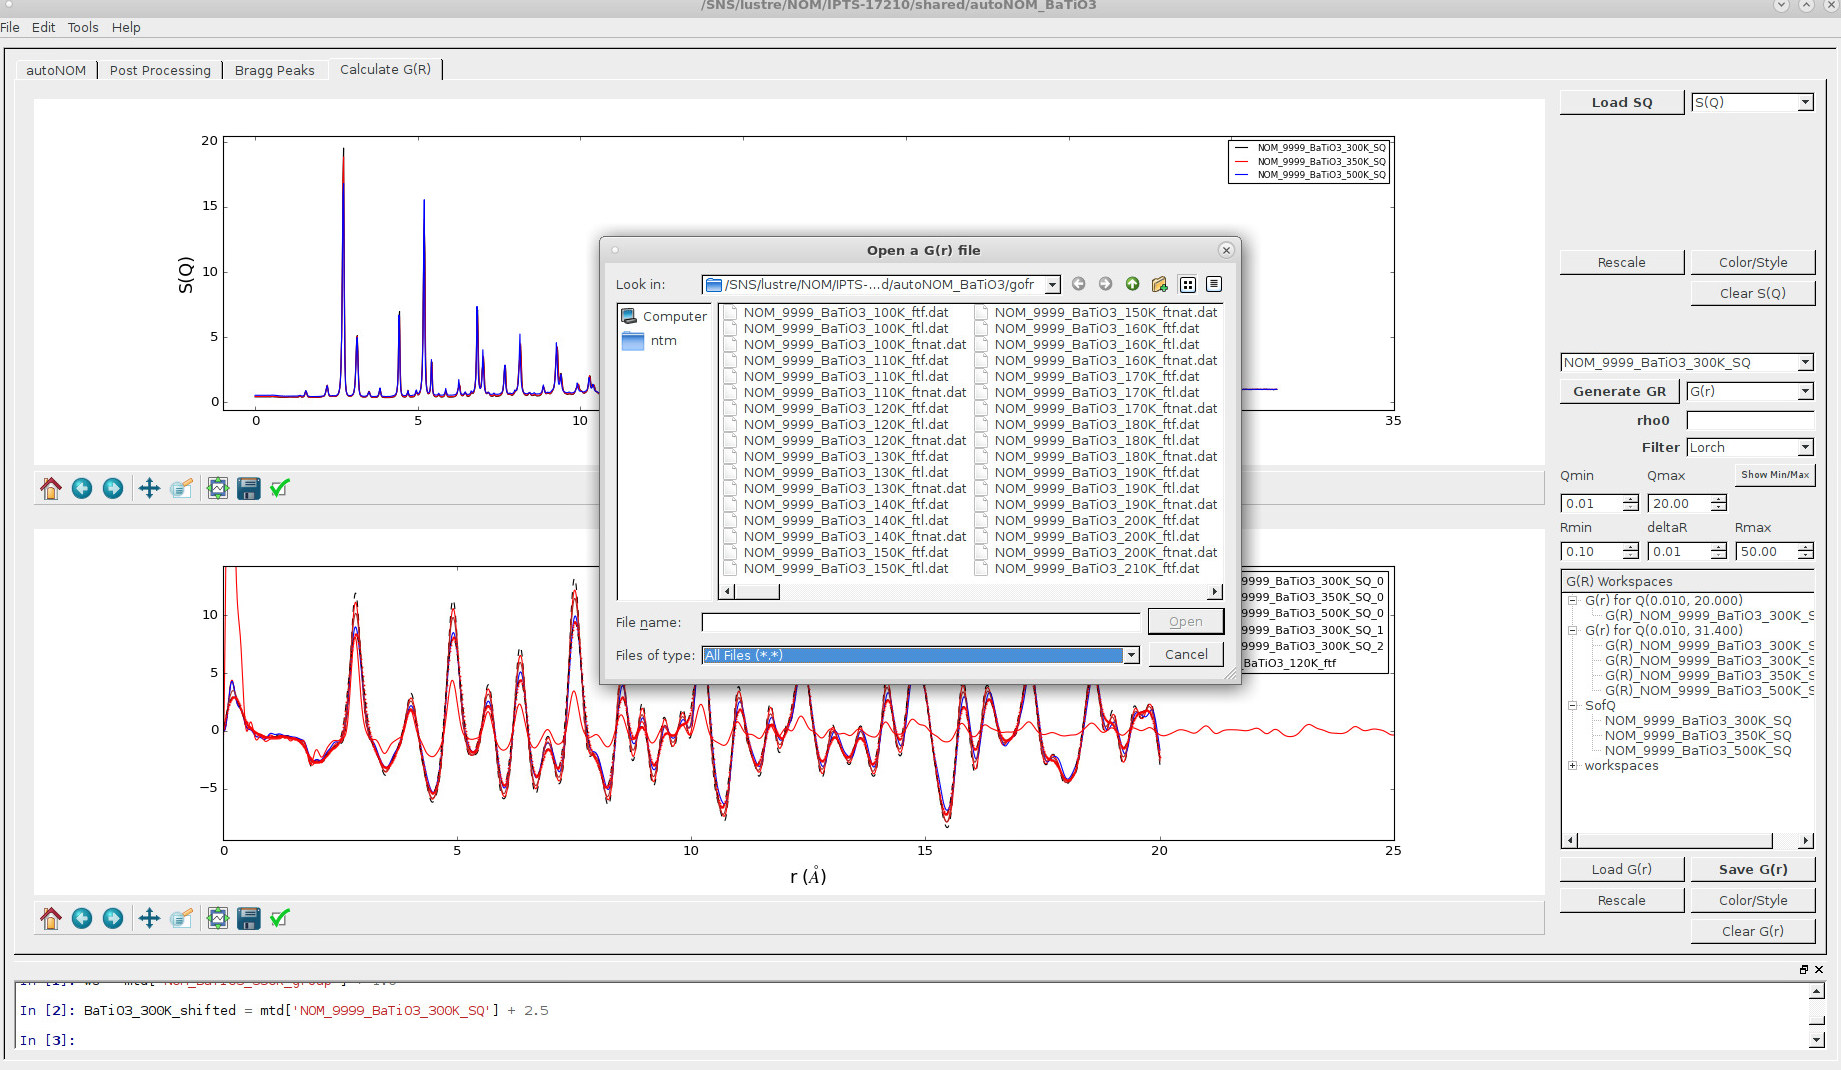
\includegraphics[width=0.9\paperwidth]{graphics/tab4/tab4_populatedGraph_loadGofR.png}}

If you choose the \fileio{gofr}, you should be presented with a file dialog similar to the one below:

\noindent\makebox[\textwidth]{\includegraphics[width=0.9\paperwidth]{graphics/tab4/tab4_populatedGraph_loadGofR_gofr.png}}

For the different file types of both, we have the following:

\begin{itemize}

\item NOMXXXftfrgr.gr – G(r) or PDF of your samples, ready for
analysis for PDFgui software package

\item NOMXXXftlrgr.gr – the same, but convoluted with the
Lorch function 

\item NOMXXXftl.dat, NOMXXXftf.dat – small g(r)

\end{itemize}


\subsection{Output G(r)}
The \guicmd{Save G(r)} button will allow you to output your selected G(r) workspace into a variety for file formats. Currently, you can output it to the following formats:

\noindent\makebox[\textwidth]{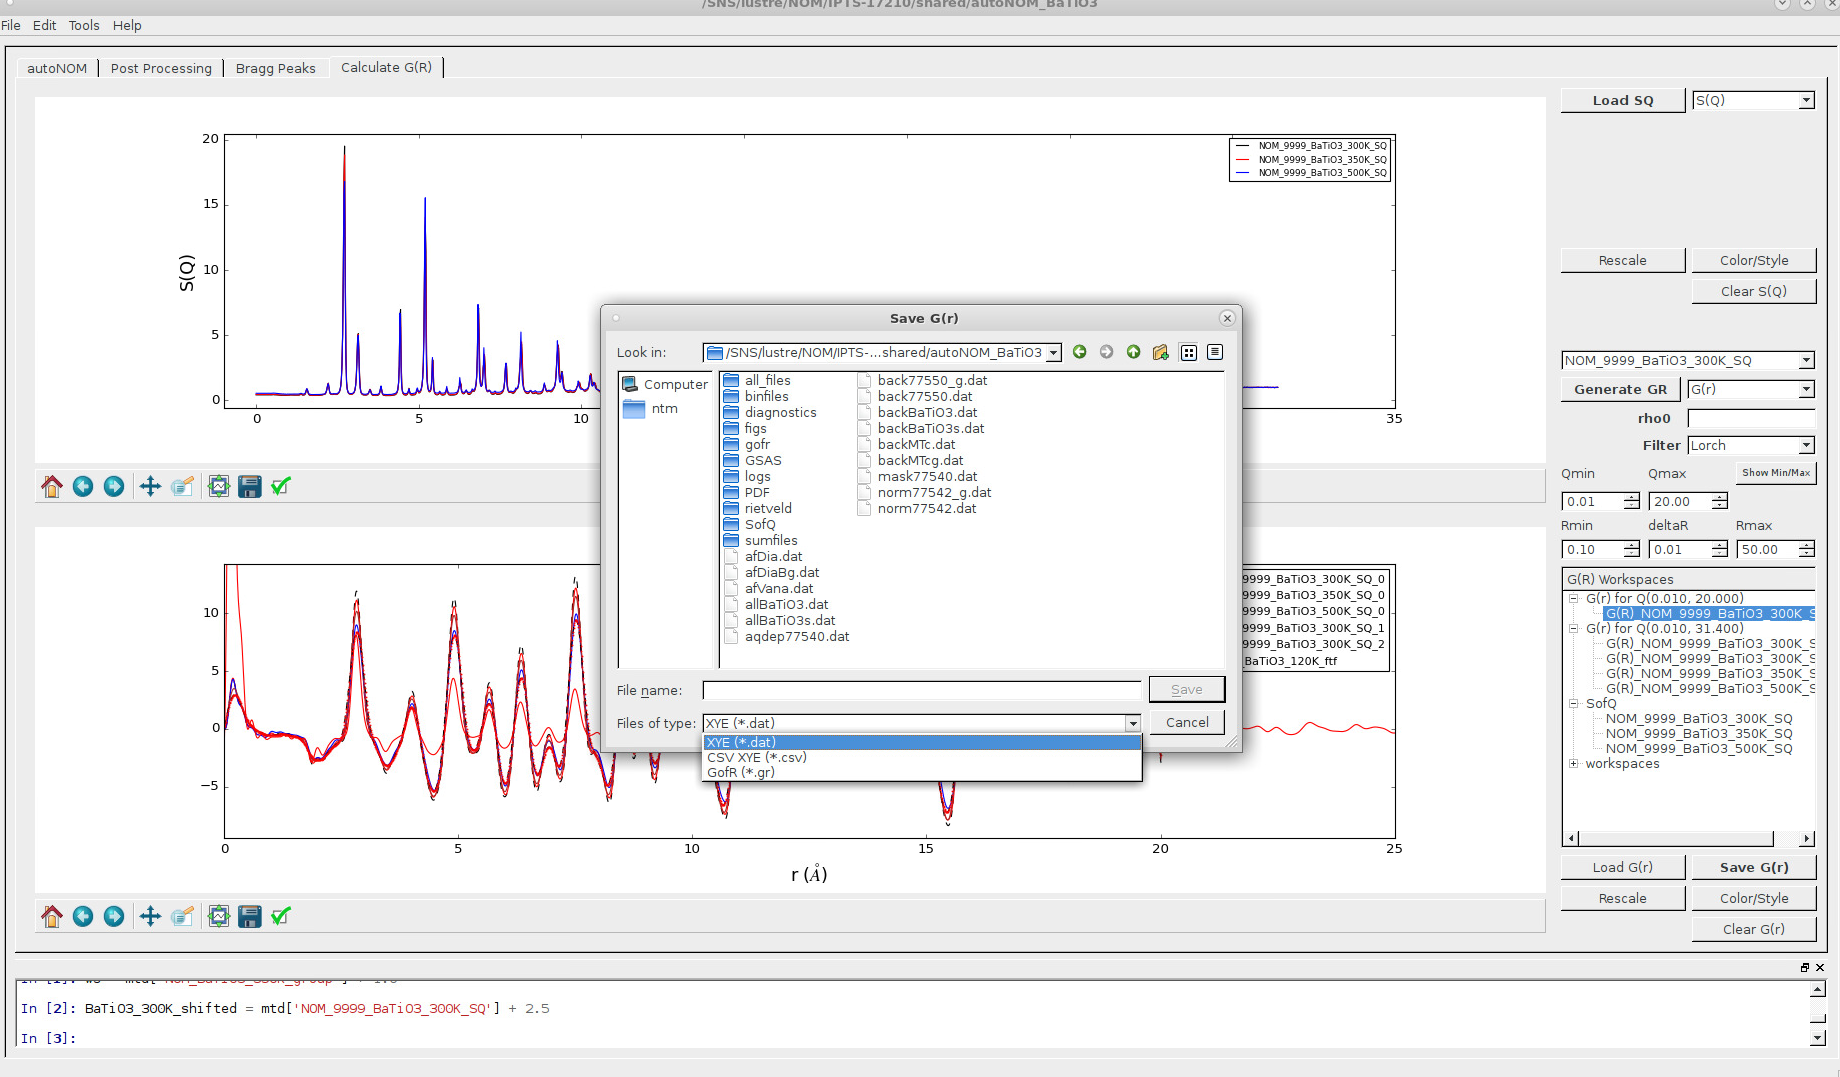
\includegraphics[width=0.9\paperwidth]{graphics/tab4/tab4_populatedGraph_saveGofR.png}}


\subsection{Optimize G(r)}

\textbf{Insert the optimization strategies we have discussed for each instrument scientist's method}






\end{document}
